\documentclass{article} 

%\usepackage{amsmath,amsthm,amsfonts}
\usepackage[bulgarian]{babel}
\usepackage[numbers]{natbib}
\usepackage{rotating}
\usepackage{amsfonts,amsmath}
\usepackage{graphicx}
\usepackage{color} 
\usepackage[notref,notcite]{showkeys}
\usepackage{multirow}
\usepackage[utf8]{inputenc}
\usepackage[T2A]{fontenc}
%\usepackage[outdir=./]{epstopdf}
\usepackage{epstopdf}
\usepackage{wrapfig}
\usepackage{placeins}

\newcommand{\be}{\begin{equation}}
\newcommand{\ee}{\end{equation}}
\newcommand{\rf}[1]{(\ref{#1})}
\newcommand{\RR}{\mathbb{R}}
\newtheorem{thm}{Theorem}
\newtheorem{lm}{Lemma}

\newcommand{\eeth}{\rm}
\newcommand{\dO}{\partial\Omega_{h}}

\begin{document}

\section{Въведение.}\label{introduction}

Тук се разглежда двумерното уравнение на Бузинеск (УБ)
\begin{align}
&u_{tt} - \Delta u -\beta_1  \Delta u_{tt} +\beta_2 \Delta ^2 u + \Delta f(u)=0   \quad \text{for}  (x,y) \in \RR^2, \, t\in\RR^+,\label{eq1}
\\ \nonumber &u(x,y,0)=u_0(x,y), \, u_t(x,y,0)=u_1(x,y)   \quad\text{for} \, (x,y) \in \RR^2,
\\  &u(x,y) \rightarrow 0,  \Delta u(x,y) \rightarrow 0 ,  \quad \text{for}  \sqrt{x^2 + y^2} \rightarrow \infty, \label{eq11}
\end{align}
където $f(u)=\alpha u^2$, $\beta_1>0$, $\beta_2>0$ са дисперсионни параметри,  $\alpha>0$ е амплитудата, а $\Delta$ е оператора на Лаплас. Извеждането на уравнението от оригиналната система е направено в \cite{ChChr}. Целта на настоящия труд е да потърси решения на \rf{eq1} от вида $u(x,y,t)=U(x,y-ct)$, който са стационарни солитонни вълни (ССВ) движещи се по $y$ оста със скорост $c$. В последствие тези вълни ще служат за начално условие на хиперболичното (УБ) \rf{eq1} -- \rf{eq11}. Важно е да получим начално условие с добра точност чрез един гъвкав и устойчив процес, който ще позволи тестването на повече и различни сценарии. Предисторията на изчисляването на ССВ за уравнение \rf{eq1} е свързана с няколко числени техники, както следва. Спектрален метод на Галеркин е изполван в \cite{chr-chr-07,chr-chr}. Шаблони с крайни разлики от втори порядък са приложени в \cite{Ch2012}. Пертурбационно решение с развитие в ред около малък параметър (скоростта) $c$ е представено в  \cite{Ch2011}, а в последствие полученият числен резултат е апроксимиран с подходящи формули в \cite{Ch2011}. Последните алгебрични изрази са използвани като начално условие за числени симулации на нестабилното УБ \rf{eq1} -- \rf{eq11}, (виж  \cite{cher,dani}). Всички тези статии показват, че при стойности на скоростта $c<0.3$, ССВ се разсейват във формата на разширяваща се пръстеновидна вълна или избухват след кратък период от време. Вижда се, че баланса между дисперсията и нелинейността в УБ \rf{eq1} е много крехък, което изисква повече усилия при запазването му. Също така е добре известно, че в едномерния случай солитонните вълни са нестабилни за малки скорости $c$ около нулата и стабилни за по-големи скорости близки до допустимия максимум $min\{1, 1/\sqrt{\beta_1/\beta_2}\}$.
Тези наблюдения изместват фокуса към изчисляване на ССВ $U$ от \rf{eq1} с по-голяма точност и при скорости $c > 0.7$, тъй като това е от съществено значение за конструирането на началните данни при нестабилното УБ \rf{eq1}. 
След полагане на $U(x,y-ct)=u(x,y,t)$ в \rf{eq1}, ССВ удовлетворяват следното нелинейно елиптично диференциално уравнение от четвърти ред

\begin{equation}\label{eq2}
c^2 (E-\beta_1 \Delta) U_{yy} = \Delta U -\beta_2 \Delta^2 U - \Delta f(U),
\end{equation}
където $E$ е тъждествения оператор. Решението на \rf{eq2} се изчислява с помощта на стъпките описани в \cite{Ch2012,chd-chr}, но са използвани допълнителни техники, които да гарантират за по-високите изисквания, който са изложени по-горе.
Първо, за численото решение на \rf{eq2} е използвана равномерна мрежа с еднаква стъпка $h_x$ = $h_y$ = $h$ в числената област $\Omega_h$ вместо неравномерна мрежа. Решението от \rf{eq2} се използва за начално условие в хиперболичната задача \rf{eq1} и е необходима по-гъста мрежа по цялото протежение на областта през която максимумът на вълната преминава. Това дава достатъчно мотивация да се използва равномерна стъпка навсякъде в областта като в допълнение ще получим повече инфомрация по границата $\partial \Omega_h$. Числените експерименти показват, че допълнителните апроксимации върху вече съществуващо решение от елиптичната задача (напр. при неравномерна мрежа с помощта на интерполация да се получат точките в равномерна мрежа) не водят до добър резултат. Мрежата и при двете задачи трябва да е една и съща.
Второ, приложени са крайни разлики с локална апроксимация от втори $O(h^2)$, четвърти $O(h^4)$ и шести $O(h^6)$ порядък, които апроксимират вторите производни по пространството. Това спомага за изчисляване на решението с по - голяма точност и дава възможност за използване на по - рехава мрежа в определени сценарии.

%A new boundary condition on the computational boundary is also used \cite{bnd}, together with uniform grid and local approximation order of $O(h^4)$ and $O(h^6)$. The numerical solution %of the fourth order elliptic problem \rf{eq2} is replaced with an iterative procedure, which involves solution  of an appropriate  parabolic type problem at every iteration step.
 %until this solution converges. 
Трето, добавен е стоп критерии, които отчита първо, остатъка от дискретното уравнение, дефиниран в \rf{residual}, второ, разликата между две решения получени от последователни итерации и трето, промяната в поведението на търсената функция в пограничните области близо до $\partial \Omega_h$.
Четвърто, разгледани са две гранични условия: нулево и ненулево като последното е описано в \cite{bnd}.
Най-накрая решенията получени от елиптичната задача са сравнени с числените резултати от \cite{Ch2012,Ch2011} при различни скорости $c$ и дисперсионни параметри $\beta =\beta_1  / \beta_2$ и е показано, че формата на решението се изменя по сходен начин и в двата случая в зависимост от входните параметри. Получените резултати от елиптичната задача са сравнени с "best-fit" апроксимационните формули изведени в \cite{Ch2011}. Показано е че последните не удовлетворяват уравнението в околност на нулата $(0,0)$ в класическия смисъл, защото четвъртите производни от решението са сингулярни. Разликата (измерена в $L_2$ и $L_\infty$ норми) между полученото тук решение и при апроксимационните формули от \cite{Ch2011} са достатъчно големи особено при по високи скорости $c$.
%\iffalse

\section{Дискретизация}
Неограничената област на уравнението е заменена с достатъчно голям правоъгълник $\Omega$, така че стойностите на неизвестната функция $u$ са достатъчно малки близо до границата $\partial \Omega$. Използвана е равномерна мрежа  $\Omega_h$ дефинирана по следния начин:

\begin{align}\label{Omega}
\Omega_h = \{(x_i,y_j): x_i = (i-\frac{N_x-1}{2})h, \; &y_j = (j-\frac{N_y-1}{2})h, \nonumber\\
                                         & i = 0,\cdots, N_x-1, j = 0 ,\cdots , N_y-1 \},
\end{align}
където $N_x$ и $N_y$ описват броя на точките по осите $x$ и $y$, а стъпката по пространството $h$ удовлетворява $h =2 L_x/(N_x-1) =2 L_y/(N_y-1)$.
С $2 L_x$ и $2 L_y$ са означени размерите на $\Omega_h$ по осите $x$ и $y$. Дискретния времеви интервал е дефиниран аналогично чрез
$$
T_{\tau} = \{(t_k): t_k = k\tau, k = 0,\cdots ,N_t-1 \},
$$
където $N_t$ е броя на точките по оста $t$, а $\tau = T/(N_t-1)$ е стъпката по времето. Стойността на неизвестната функция $u$ в точка от мрежата $(x_i,y_j,t_k)$ е означена с $u_{i,j}^{(k)}$,т.е. долният индекс се използва за пространствена дискретизация, а горният за времева. За дискретизация на оператора на Лаплас са използвани централни крайни разлики с различна степен на апроксимация:
\begin{equation}\label{fdx}
u_{\widehat{xx},p}(x,y) :=  \frac{1}{h^2} \sum\limits_{i=-p/2}^{p/2} d_i u(x+ih, y_j).
\end{equation}
като теглата $d_i$ са взети от \cite{forn} и са описани в Таблица \ref{table:A00}. Производните по $y$ се дефинират аналогично със същия шаблон:
\begin{equation}\label{fdy}
u_{\widehat{yy},p}(x,y) :=  \frac{1}{h^2} \sum\limits_{i=-p/2}^{p/2} d_i u(x, y_j+ih).
\end{equation}

\begin{table}[ht]
\centering
\small
		\begin{tabular}{||c|l|l|l|l|l|l|l||}
			\hline
			\hline
            $p=2$          &          &                                 &     1      &   -2   &    1    &    &        \\
   			\hline 
			\hline 
           $p=4$          &                            &   $-\frac{1}{12}$     &     $\frac{4}{3}$      &   $-\frac{5}{2} $     &    $\frac{4}{3}$    &  $-\frac{1}{12}$   &        \\
	   \hline
			\hline 
            $p=6$        &   $\frac{1}{90}$       &     $-\frac{3}{20}$     &    $\frac{3}{2}$      &    $-\frac{49}{18}$   &    $\frac{3}{2}$    & $-\frac{3}{20}$    &    $\frac{1}{90}$       \\
	   \hline
			\hline 
		\end{tabular}
	\caption{Централни крайни разлики използвани при апроксимацията на оператора на Лаплас.}
	\label{table:A00}
\end{table}
Грешката от дискретните апроксимации \rf{fdx}, \rf{fdy} е $O(h^p)$ в зависимост от избора на $p$. Използвайки мрежата $\Omega_h$ и Таблица \ref{table:A00} при $p=2$ може да се дефинират следните диференчни оператори:
\begin{align}
u_{\bar{x}x}(x_i,y_j) = u_{\widehat{xx},2}(x_i,y_j) = \frac{1}{h^2}(u_{i+1,j} - 2u_{i,j} + u_{i-1,j}), i = 1,.., N_x-2, j = 0,.., N_y-1 \nonumber\\
u_{\bar{y}y}(x_i,y_j) = u_{\widehat{yy},2}(x_i,y_j) = \frac{1}{h^2}(u_{i,j+1} - 2u_{i,j} + u_{i,j-1}), i = 0,.., N_x-1, j = 1,.., N_y-2. \nonumber
\end{align}
Производните по времето в $T_{\tau}$ са съответно:
\begin{align}
& u^{(k)}_{\bar{t}t}(x_i,y_j,t_k) = \frac{1}{\tau^2}(u_{i,j}^{(k+1)} - 2u_{i,j}^{(k)} + u_{i,j}^{(k-1)}), k = 1,..,N_t-2 \nonumber\\
& u^{(k)}_{t}(x_i,y_j,t_k) =  \frac{1}{\tau}(u_{i,j}^{(k+1)} - u_{i,j}^{(k)}), k = 0,.., N_{t}-2 \nonumber\\
& u^{(k)}_{\bar{t}}(x_i,y_j,t_k) =  \frac{1}{\tau}(u_{i,j}^{(k)} - u_{i,j}^{(k-1)}), k = 1,.., N_{t}-1 \nonumber.
\end{align}
Дискретния оператор на Лаплас в произволна точка от вътрешността на мрежата $(x_i, y_j) \in \Omega_h \setminus \partial\Omega$ се изразява с 
$$\Delta_{h,2}u(x_i, y_j, t_k) :=  u_{\bar{x}x}(x_i, y_j, t_k) + u_{\bar{y}y}(x_i, y_j, t_k),$$
а при произволно $p$ важи следната дефиниция:
\be\label{deltaHSingle}
\Delta_{h,p} u(x_i, y_j, t_k) :=  u_{\widehat{xx},p}(x_i, y_j, t_k) + u_{\widehat{yy},p}(x_i, y_j, t_k).
\ee
Последното уравнение може да се запише в матричен вид отчитайки всички вътрешни точки от мрежата. За целта се дефинира следната помощна редица от матрици $\left(V^{(k)}\right) := (u_{i,j}^{(k)})$ при $k=0,..,N_t$. Колоните в тази матрица изобразяват неизвестната функция по $x$-оста, а редовете - неизвестната функция по $y$-оста. Така за дискретния оператор на Лаплас $\Delta_h$ се получава, че: 
\be\label{DeltaH}
\Delta_{h,p} (V^{(k)})  := \Delta_{h,p,x}*V^{(k)} + \left( \Delta_{h,p,y} * (V^{(k)})^T \right)^T,
\ee
където $\Delta_{h,p,x}\in \RR^{(N_x-2) \times (N_x-2)}$ и $\Delta_{h,p,y}\in \RR^{(N_y-2) \times (N_y-2)}$ са квадратни лентови матриции с една и съща структура, но с различна големина, a $(.)^T$ е транспонирата матрица. При $p=2$ и произволно естествено число $n>2$ се получава
\[
\Delta_{h,2,n} = \frac{1}{h^2}
\begin{bmatrix}
    \dots       & \dots        &     \dots   &   \dots        & 0   \\
    1               & -2            &   1           &   0               & \vdots    \\
        0           & \ddots        &    \ddots    &   \ddots       &  0 \\ 
    \vdots       &     0            &  1     	& -2    	   & 1 \\
    0               & \dots          &  \dots         & \dots  	   & \dots \\
\end{bmatrix}
\in \\R^{n^2}
\]
При $p=4$ и произволно естествено число $n>4$ 
\[
\Delta_{h,4,n} = \frac{1}{h^2}
\begin{bmatrix}
    \dots		& \dots            	& \dots		&   		 \dots  &    \dots      	   &   0           & 0    \\
    \dots    	           &\dots            	& \dots		&   		\dots   &   \dots      	   	   &   0	           & \vdots  \\
    -\frac{1}{12}	& \frac{4}{3}         	& -\frac{5}{2}	&  \frac{4}{3}    	 &   -\frac{1}{12}	  &      0           &\vdots    \\
        0           		& \ddots        	&    \ddots   		 &   \ddots      	 &     \ddots      	  &  \ddots        &    0 \\	
\\
   \vdots      		 & 0           		 &  -\frac{1}{12}	& \frac{4}{3}    	& -\frac{5}{2}	&  \frac{4}{3}  &   -\frac{1}{12} \\
    \vdots    		 & 0        		 &	 \dots     	&  \dots              	&\dots 		 &  \dots 	&\dots   	\\
    0              		 & 0        		 &	 \dots     	&  \dots             	 &\dots 		 &  \dots 	&\dots 	\\
\end{bmatrix}
\in \\R^{n^2}
\]
При $p=6$ и произволно естествено число $n>6$ е показана само структурата на лентата  (виж Таблица \ref{table:A00}):
\[
\begin{bmatrix}
    \frac{1}{90}	& -\frac{3}{20}	& \frac{3}{2}         	& -\frac{49}{18}	&  \frac{3}{2}    	 &   -\frac{3}{20}	  &      \frac{1}{90}
\end{bmatrix}
\]
като тук първите три и последни три реда от матрицата са все още предмет на дефиниране, т.е. в хоризонталните многоточия на горепосочените матрици $\Delta_{h,p,n}$ трябва да се дефинира граничното условие заложено в ПУБ по подходящ начин.

\section{Нулево гранично условие}
Пространството от функции, за които е изпълнено $f_b(x) = 0$ и $\Delta f_b(x) = 0$ по границата $\partial\Omega$ се дефинира чрез
\be\label{funSpace}
J_\infty:=\{ f_b : \Omega \rightarrow R | f_b(x) = 0, \Delta f_b(x) = 0, x \in \partial\Omega\}
\ee
Това пространство е в съответстие на граничните условия зададени в ПУБ. Дискретните оператори $\Delta_{h,p,x} \in \RR^{(N_x-2) \times (N_x-2)}$ и $\Delta_{h,p,y} \in \RR^{(N_y-2)\times(N_y-2)}$  използват централни крайни разлики с 3, 5 и 7 точки съответно при различните апроксимации $O(h^2)$, $O(h^4)$ и $O(h^6)$ на вторите производни. По и близо до границата се прилагат други шаблони възползвайки се от свойствата на функционалното пространство. При $p=2$ имаме, че 
\[
\Delta_{h,2,x} = \frac{1}{h^2}
\begin{bmatrix}
    -2	       & 1        &     \dots   &   \dots        & 0   \\
    1               & -2            &   1           &   0               & \vdots    \\
        0           & \ddots        &    \ddots    &   \ddots       &  0 \\ 
    \vdots       &     0            &  1     	& -2    	   & 1 \\
    0               & \dots          &  \dots         & 1  	   & -2 \\
\end{bmatrix},
\]
защото $u \in J_\infty$ и $u(x_0, y_j, t_k) = u(x_{N_x}, y_j, t_k) = 0$. По същия начин, но с различна големина, изглежда и матрицата $\Delta_{h,p,y}$, защото $u \in J_\infty$ и $u(x_i, y_0, t_k) = u(x_i, y_{N_y}, t_k) = 0$.  При $p=4$ имаме, че 
\[
\Delta_{h,4,x} = \frac{1}{h^2}
\begin{bmatrix}
     -\frac{38}{15}	& \frac{29}{20}       & -\frac{2}{15}	&    \frac{1}{120}     &    \dots      	   &   0           & 0    \\
    \frac{4}{3}          &-\frac{5}{2}    	& \frac{4}{3}	&   -\frac{1}{12}	  &   \dots      	  &   0	           & \vdots  \\
    -\frac{1}{12}	& \frac{4}{3}         	& -\frac{5}{2}	&  \frac{4}{3}    	 &   -\frac{1}{12}	  &      0           &\vdots    \\
        0           		& \ddots        	&    \ddots   		 &   \ddots      	 &     \ddots      	  &  \ddots        &    0 \\	
\\
   \vdots      		 & 0           		 &  -\frac{1}{12}	& \frac{4}{3}    	& -\frac{5}{2}	&  \frac{4}{3}   &   -\frac{1}{12} \\
    0      		 &  \dots           	 &   0     		& -\frac{1}{12} 	 & \frac{4}{3} 	 & -\frac{5}{2}  &  \frac{4}{3}\\
    0              		 & \dots          	&  0              		 &\frac{1}{120} 	 &  -\frac{2}{15} 	& \frac{29}{20} & -\frac{38}{15}\\
\end{bmatrix}
\]
Вторият и предпоследният редове на матрицата $\Delta_{h,4,x}$ се обясняват с условието, че $u \in J_\infty$ и съответно $u(x_0, y_j, t_k) = u(x_{N_x}, y_j, t_k) = 0$ както е при $O(h^2)$ апроксимацията. 

\begin{figure}%{r}{50mm}
     \begin{center}
     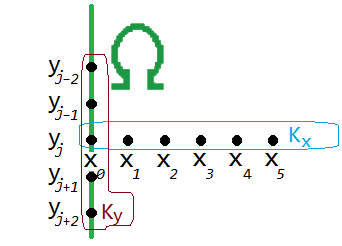
\includegraphics[scale=.5]{LeftBoundary.png}
     \end{center}
	\caption{Шаблон с $O(h^4)$ апроксимация при имплементация на $\Delta_h$ оператора по лявата граница на областта.}
	\label{fig:LeftBoundary}
\end{figure}

Условието $\Delta u(x_0, y, t) = 0$ върху лявата граница на областта се описва с крайна разлика напред $K_x[0,1,2,3,4,5]$ за втората производна по $x$ и централна крайна разлика $K_y[-2,-1,0,1,2]$ за втората производна по $y$ (виж Фигура \rf{fig:LeftBoundary}). С вектора в квадратните скоби на крайните разлики $K_x$ и $K_y$ се обозначава релативната позиция на използваните възли. Резултатът от произвнодните пресметнати посредством $K_x$ и $K_y$ се отнася за възела обозначен с нула. Понеже $u(x_0, y, t) = 0$ следва, че събираемите от $K_y[-2,-1,0,1,2]$ заедно с първия елемент от $K_x[0,1,2,3,4,5]$ са нула. Като последното важи за всяка крайна разлика $K_y$ с точки върху границата $\partial \Omega$. Ако означим с $\bar c_0, \bar c_1, .., \bar c_5$ теглата на крайната разлика напред $K_x[0,1,2,3,4,5]$ и с $\bar d_0, \bar d_1,.., \bar d_5$ теглата на крайната разлика $K_x[-1,0,1,2,3,4]$ се получава че:
\begin{align}
\sum\limits_{i=0}^{5} \bar c_i u(x+ih, y_j) = \sum\limits_{i=1}^{5} \bar c_i u(x+ih, y_j) = 0 &  \quad | \frac{\bar d_5}{\bar c_5} \nonumber\\
\bar d_5 u(x+5h, y_j) = -\sum\limits_{i=1}^{4} \bar c_i u(x+ih, y_j) & \nonumber
\end{align}
Последният член $u(x+5h, y_j)$ от $K_x[0,1,2,3,4,5]$ е изразен чрез останалите и може да се замести в $K_x[-1,0,1,2,3,4]$ както следва:
\begin{align}\label{fdResult}
&\sum\limits_{i=0}^{5} \bar d_i u(x+ih, y_j) = \sum\limits_{i=1}^{5} \bar d_i u(x+ih, y_j)  =  \\
&= \sum\limits_{i=1}^{4} \bar d_i u(x+ih, y_j) -\sum\limits_{i=1}^{4} \bar c_i u(x+ih, y_j) = \sum\limits_{i=1}^{4} \left( \bar d_i - \frac{\bar d_5}{\bar c_5} \bar c_i \right) u(x+ih, y_j) \nonumber
\end{align}
Понеже $K_x[0,1,2,3,4,5]$ и $K_x[-1,0,1,2,3,4]$ са крайни разлики апроксимиращи втора производна с грешка $O(h^4)$ (\cite{forn}) то полученият резултат \rf{fdResult} е със същата грешка $O(h^4)$. Теглата $\bar c_i$ и $\bar d_i$ при $p=4$ са дефинирани както следва (\cite{forn}):
\begin{align}
&\bar c_i, i = 0,..,5 \iff \frac{15}{4}, -\frac{77}{6}, \frac{107}{6}, -13, \frac{61}{12}, -\frac{5}{6} \\
&\bar d_i, i = 0,..,5 \iff \frac{5}{6}, -\frac{5}{4}, -\frac{1}{3}, \frac{7}{6}, -\frac{1}{2}, \frac{1}{12} 
\end{align}
и след като се заместят в \rf{fdResult} се получават коефициентите от първия ред на матрицата $\Delta_{h,4,x}$. При последния ред се прилагат аналогични разсъждения върху дясната граница на областта, но вече се използва крайна разлика назад $K_x[-4,-3,-2,-1,0]$ за втората производна по $x$ при пресмятането на дискретния Лапласиан. 

Аналогични разсъждения се прилагат за горната и долната граници на областта при другата матрица $\Delta_{h,4,y}$, която се използва за изчисляването на втората производна по $y$ и затова нейната структура е същата.

При $p=6$ матрицата $\Delta_{h,6,x}$ има следния вид:
\[
\frac{1}{h^2}
\begin{bmatrix}
   -\frac{327}{140}	& \frac{191}{168}	&   \frac{167}{1134}	& -\frac{1}{7}    		 & \frac{19}{420}	& -\frac{77}{13331}   &    0      	   	&   \dots           & 0    \\
    \frac{54}{35}    	&-\frac{235}{84}   	&    \frac{884}{567}    &-\frac{5}{28}  	 	& \frac{2}{105}		&  -\frac{11}{11340}	 &   0      	   	&   \dots	       & \vdots  \\
    -\frac{3}{20}		& \frac{3}{2}         	& -\frac{49}{18} 	&  \frac{3}{2}		&  -\frac{3}{20}    	 &   \frac{1}{90}    	 &  0			&     \dots         &\vdots    \\
    \frac{1}{90}		& -\frac{3}{20}		& \frac{3}{2}         	& -\frac{49}{18} 	&  \frac{3}{2}		&  -\frac{3}{20}    	 &   \frac{1}{90} &     \dots         &\vdots    \\
        0           		& \ddots        		&         \ddots           	& \ddots        		&    \ddots   		&   \ddots      		 &     \ddots    	&  \ddots          &    0 \\	
\\
   \vdots      		&            		 	&    	0	      		& \frac{1}{90}		& -\frac{3}{20}		& \frac{3}{2}         	& -\frac{49}{18}	&  \frac{3}{2}  &  -\frac{3}{20} \\
    0      			&              	 	&    0      		&   -\frac{11}{11340}	 	&    \frac{2}{105} 	&  -\frac{5}{28} 	& \frac{884}{567} &-\frac{235}{84} &  \frac{54}{35}\\
    0              	& 	          		&    0              	&  -\frac{77}{13331}    		&  \frac{19}{420}&-\frac{1}{7}	 &  \frac{167}{1134} 	& \frac{191}{168}  &  -\frac{327}{140}\\
\end{bmatrix}
\]
Третият и предпредпоследният ред на матрицата $\Delta_{h,6,x}$ сa следствие от факта, че $u \in J_\infty$ и съответно $u(x_0, y_j, t_k) = u(x_{N_x}, y_j, t_k) = 0$ както е при $O(h^2)$ апроксимацията. 


Условието $\Delta u(x_0, y, t) = 0$ върху лявата граница на областта се описва с крайна разлика напред $K_x[0,1,2,3,4,5,6,7]$ за втората производна по $x$ и централна крайна разлика $K_y[-3,-2,-1,0,1,2,3]$ за втората производна по $y$ както е направено при $p=4$ (виж Фигура \rf{fig:LeftBoundary}), но с разликата че тук по-високият порядък на апроксимация изисква два възела в повече. Понеже $u(x_0, y, t) = 0$ следва, че събираемите от $K_y[-3,-2,-1,0,1,2,3]$ заедно с първия елемент от $K_x[0,1,2,3,4,5,6,7]$ са нула. Като последното важи за всяка крайна разлика $K_y$ с точки върху границата $\partial \Omega$. Ако означим с $\bar c_0, \bar c_1, .., \bar c_7$ теглата на крайната разлика напред $K_x[0,1,2,3,4,5,6,7]$ и с $\bar d_0, \bar d_1,.., \bar d_7$ теглата на крайната разлика $K_x[-1,0,1,2,3,4,5,6]$ се получава че:
\begin{align}\label{deltaOh6Zero}
\sum\limits_{i=0}^{7} \bar c_i u(x+ih, y_j) = \sum\limits_{i=1}^{7} \bar c_i u(x+ih, y_j) = 0 &  \quad | \frac{\bar d_7}{\bar c_7} \nonumber\\
\bar d_7 u(x+7h, y_j) = -\sum\limits_{i=1}^{6} \bar c_i u(x+ih, y_j) & 
\end{align}
Последният член $u(x+7h, y_j)$ от $K_x[0,1,2,3,4,5,6,7]$ е изразен чрез останалите и може да се замести в $K_x[-1,0,1,2,3,4,6]$ както следва:
\begin{align}\label{fdResultOh6}
&\sum\limits_{i=0}^{7} \bar d_i u(x+ih, y_j) = \sum\limits_{i=1}^{7} \bar d_i u(x+ih, y_j)  =  \\
&= \sum\limits_{i=1}^{6} \bar d_i u(x+ih, y_j) -\sum\limits_{i=1}^{6} \bar c_i u(x+ih, y_j) = \sum\limits_{i=1}^{6} \left( \bar d_i - \frac{\bar d_7}{\bar c_7} \bar c_i \right) u(x+ih, y_j) \nonumber
\end{align}
Понеже $K_x[0,1,2,3,4,5,6,7]$ и $K_x[-1,0,1,2,3,4,5,6]$ са крайни разлики апроксимиращи втора производна с грешка $O(h^6)$ (\cite{forn}) то полученият резултат \rf{fdResultOh6} е със същата грешка $O(h^6)$. Теглата $\bar c_i$ и $\bar d_i$ при $p=6$ са дефинирани както следва (\cite{forn}):
\begin{align}
&\bar c_i, i = 0,..,7 \iff \frac{469}{90}, -\frac{223}{10}, \frac{879}{20}, -\frac{949}{18}, 41, -\frac{201}{10}, \frac{1019}{180}, -\frac{7}{10} \\
&\bar d_i, i = 0,..,7 \iff \frac{7}{10}, -\frac{7}{18}, -\frac{27}{10}, \frac{19}{4}, -\frac{67}{18}, \frac{9}{5}, -\frac{1}{2}, \frac{11}{180}
\end{align}
и след като се заместят в \rf{fdResultOh6} се получават коефициентите от първия ред на матрицата $\Delta_{h,6,x}$. 
Ако пък с $\bar d_0, \bar d_1, .., \bar d_7$ се означат теглата в $K_x[-2,-1,0,1,2,3,4,5]$ и се използва резултата от \rf{deltaOh6Zero} то тогава в \rf{fdResultOh6} се получават коефициентите от втория ред в  $\Delta_{h,6,x}$. Коефициентите при $K_x[-2,-1,0,1,2,3,4,5]$ са:
\begin{align}
&\bar d_i, i = 0,..,7 \iff -\frac{11}{180}, \frac{107}{90}, -\frac{21}{10}, \frac{13}{18}, \frac{17}{36}, -\frac{3}{10}, \frac{4}{45}, -\frac{1}{90}
\end{align}
За да се построи долната дясна част на матрцата се подхожда както до сега при горната лява част. Аналогични разсъждения се прилагат за горната и долната граници на областта при другата матрица $\Delta_{h,6,y}$, която се използва за изчисляването на втората производна по $y$, където отново се получава същата структура.

\section{Симетрично гранично условие по абцисата и ординатата при елиптичната задача}
Нейзвестната функция $u$ клони към нула на безкрайност, но е показано, че решенията от стационарната задача са симетрични по $x$ и $y$ осите. Това позволява да се търси решение само в първи квадрант. Симетричното условие може да се построи посредством следния запис
\begin{align}\label{funSpaceSym}
J_s:=\{ f_s : \Omega \rightarrow \RR  \; | \; f_s(x_i,y_j) = f_s(x_i,-y_j), f_s(x_i,y_j) = f_s(-x_i,y_j),\nonumber\\
(x_i,y_j) \in \omega_h, \; (x_i,-y_j), (-x_i,y_j) \in \Omega_h\}.
\end{align}
Търсената функция изпълнява условието, че $u(x_i,y_j) \in J_\infty \cap J_s$, но ще разгледаме уравнението само в $\omega_h \in \Omega_h$. Дискретните оператори $\Delta_{h,p,x} \in \RR^{(N_x-2) \times (N_x-2)}$ и $\Delta_{h,p,y} \in \RR^{(N_y-2)\times(N_y-2)}$ дефинирани в ``Нулево гранично условие''  ще бъдат от помощ при построяването на $\Delta_{h,p,s,x} \in \RR^{(N_x-1)/2 \times (N_x-1)/2}$ и $\Delta_{h,p,s,y} \in \RR^{(N_y-1)/2\times(N_y-1)/2}$ описващи симетричното условие по абцисата и ординатата в $\omega_h$:
\be\label{PsnDiscretSym}
\Delta_{h,p,s}(v^{(k)}) := \Delta_{h,p,s,x} *  v^{(k)} + v^{(k)} * (\Delta_{h,p,s,y})^T.
\ee
Структурата на матриците $\Delta_{h,p,s,x}$ и $\Delta_{h,p,s,y}$ се различава от $\Delta_{h,p,x}$ и $\Delta_{h,p,y}$ само в първите $i$ редове (при $p=2$ и $i=0$, при $p=4$ и $i=0,1$, при $p=6$ и $i=0,1,2$), където е приложено условието за симетрия. Останалите редове и ненулевите елементи спрямо главните им диагонали, са едни и същи, защото апроксимират втора производна с един и същи ред на апроксимация $p$ и нулево гранично условие по границите $x=L_x$ и $y=L_y$. Така, при $p=2$ се получава, че 
\[
\Delta_{h,2,s,x} = \frac{1}{h^2}
\begin{bmatrix}
    -2	       & 2        &     \dots   &   \dots        & 0   \\
    1               & -2            &   1           &   0               & \vdots    \\
        0           & \ddots        &    \ddots    &   \ddots       &  0 \\ 
    \vdots       &     0            &  1     	& -2    	   & 1 \\
    0               & \dots          &  \dots         & 1  	   & -2 \\
\end{bmatrix}
\in \RR^{(N_x-1)/2 \times (N_x-1)/2},
\]
защото $u \in J_s$ и $u(x_1, y_j) = u(x_{-1}, y_j)$ и следователно $u(x_1, y_j) + u(x_{-1}, y_j) = 2 u(x_1, y_j)$. По същия начин, но с различна големина, изглежда и матрицата $\Delta_{h,p,s,y}$, защото $u \in J_s$ и $u(x_i, y_1) = u(x_i, y_{-1})$.  При $p=4$ имаме, че 
\[
\Delta_{h,4,s,x} = \frac{1}{h^2}
\begin{bmatrix}
     -\frac{5}{2}	& \frac{8}{3}       & -\frac{1}{6}	&    0     			&    \dots      	   &   0           & 0    \\
    \frac{4}{3}          &-\frac{31}{12}    	& \frac{4}{3}	&   -\frac{1}{12}	  	&   \dots      	  &   0	           & \vdots  \\
    -\frac{1}{12}	& \frac{4}{3}         	& -\frac{5}{2}	&  \frac{4}{3}    	 &   -\frac{1}{12}	  &      0           &\vdots    \\
        0           		& \ddots        	&    \ddots   		 &   \ddots      	 &     \ddots      	  &  \ddots        &    0 \\	
\\
   \vdots      		 & 0           		 &  -\frac{1}{12}	& \frac{4}{3}    	& -\frac{5}{2}	&  \frac{4}{3}   &   -\frac{1}{12} \\
    0      		 &  \dots           	 &   0     		& -\frac{1}{12} 	 & \frac{4}{3} 	 & -\frac{5}{2}  &  \frac{4}{3}\\
    0              		 & \dots          	&  0              		 &\frac{1}{120} 	 &  -\frac{2}{15} 	& \frac{29}{20} & -\frac{38}{15}\\
\end{bmatrix}
 \in \RR^{(N_x-1)/2 \times (N_x-1)/2}
\]
Вторият ред на матрицата $\Delta_{h,4,s,x}$ и по точно тежестта при централният възел от крайната разлика с апроксимация от 4ти ред (виж Таблица \rf{table:A00}) се изразява както следва:
$$u(x_1, y_j) = u(x_{-1}, y_j) \Rightarrow -\frac{1}{12}u(x_{-1}, y_j) -\frac{5}{2}u(x_1, y_j) = -\frac{31}{12}u(x_1, y_j) $$
с пояснението, че $u \in J_s$. Така централният възел е модифициран, първият е премахнат, а останалите са непроменени. При първия ред в $\Delta_{h,4,s,x}$ за гореспоменатата крайна разлика важат следните равенства
$$u(x_1, y_j) = u(x_{-1}, y_j), u(x_2, y_j) = u(x_{-2}, y_j).$$
От последното равенство за последните два възела се получава, че:
\begin{align}
\frac{4}{3}u(x_{-1}, y_j) +\frac{4}{3}u(x_1, y_j) = \frac{8}{3}u(x_1, y_j) \nonumber\\
-\frac{1}{12}u(x_{-2}, y_j) -\frac{1}{12}u(x_2, y_j) = -\frac{1}{6}u(x_2, y_j). \nonumber
\end{align}
Аналогични разсъждения се прилагат за границата разположена върху ординатата при $\omega_h$ за другата матрица $\Delta_{h,4,s,y} \in \RR^{(N_y-1)/2 \times (N_y-1)/2}$, която се използва за изчисляването на втората производна по $y$ и затова нейната структура е същата както при $\Delta_{h,4,s,x}$, но размерът ѝ е друг.

При $p=6$ матрицата $\Delta_{h,6,s,x}$ има следния вид:
\[
\frac{1}{h^2}
\begin{bmatrix}
   -\frac{49}{18}		& \frac{3}{1}			&   -\frac{3}{10}		& \frac{1}{45}    		 &  0					& 0	   					&    0      	   	&   \dots           & 0    \\
    \frac{3}{2}    	&-\frac{517}{180}    	&    \frac{68}{45}     & -\frac{3}{20}  	 		& \frac{1}{90} 		&  0					 &   0      	   	&   \dots	       & \vdots  \\
    -\frac{3}{20}		& \frac{68}{45}         	& -\frac{49}{18} 	&  \frac{3}{2}		&  -\frac{3}{20}    	 &   \frac{1}{90}    	 &  0			&     \dots         &\vdots    \\
    \frac{1}{90}		& -\frac{3}{20}		& \frac{3}{2}         	& -\frac{49}{18} 	&  \frac{3}{2}		&  -\frac{3}{20}    	 &   \frac{1}{90} &     \dots         &\vdots    \\
        0           		& \ddots        		&         \ddots           	& \ddots        		&    \ddots   		&   \ddots      		 &     \ddots    	&  \ddots          &    0 \\	
\\
   \vdots      		&            		 	&    	0	      		& \frac{1}{90}		& -\frac{3}{20}		& \frac{3}{2}         	& -\frac{49}{18}	&  \frac{3}{2}  &  -\frac{3}{20} \\
    0      			&              	 	&    0      		&   -\frac{11}{11340}	 	&    \frac{2}{105} 	&  -\frac{5}{28} 	& \frac{884}{567} &-\frac{235}{84} &  \frac{54}{35}\\
    0              	& 	          		&    0              	&  -\frac{77}{13331}    		&  \frac{19}{420}&-\frac{1}{7}	 &  \frac{167}{1134} 	& \frac{191}{168}  &  -\frac{327}{140}\\
\end{bmatrix}
\]
Третият ред на матрицата $\Delta_{h,6,s,x}$ се изразяват от условието, че $u \in J_s$ и съответно $u(x_1, y_j) = u(x_{-1}, y_j)$. Така за тежестта при третия възел от крайната разлика с апроксимация от 6ти ред (виж Таблица \rf{table:A00}) се получава, че:
$$ \frac{1}{90}u(x_{-1}, y_j) + \frac{3}{2}u(x_1, y_j) = \frac{68}{45}u(x_1, y_j).$$ Тук, първият възел е премахнат, третият е модифициран, а останалите са непроменени. При втория ред на матрицата $\Delta_{h,6,s,x}$ от условието за симетричност следва, че
$u(x_1, y_j) = u(x_{-1}, y_j), u(x_2, y_j) = u(x_{-2}, y_j),$
за да се получат
\begin{align}
-\frac{3}{20}u(x_{-1}, y_j) -\frac{49}{18}u(x_1, y_j) = -\frac{517}{180}u(x_1, y_j) \nonumber\\
\frac{1}{90}u(x_{-2}, y_j) +\frac{3}{2}u(x_2, y_j) = \frac{68}{45}u(x_2, y_j). \nonumber
\end{align}
Първите два възела се приспадат, съответно към петия и четвъртия, а останалите са непроменени. За първия ред симетрията се пада спрямо централния възел на крайната разлика и лесно се вижда, че
\begin{align}
\frac{1}{90}u(x_{-3}, y_j) +\frac{1}{90}u(x_3, y_j) = \frac{1}{45}u(x_3, y_j) \nonumber\\
-\frac{3}{20}u(x_{-2}, y_j) - \frac{3}{20}u(x_2, y_j) = -\frac{3}{10}u(x_2, y_j) \nonumber\\
\frac{3}{2}u(x_{-1}, y_j) + \frac{3}{2}u(x_1, y_j) = \frac{3}{1}u(x_1, y_j). \nonumber
\end{align}
Аналогични разсъждения се прилагат за границата разположена върху ординатата при $\omega_h$ за другата матрица $\Delta_{h,6,s,y} \in \RR^{(N_y-1)/2 \times (N_y-1)/2}$, която се използва за изчисляването на втората производна по $y$ и затова нейната структура е същата както при $\Delta_{h,6,s,x}$, но размерът ѝ е друг. 

\section{Инструменти използвани при числените резултати}

Реда на сходимост на изследваните крайни разлики и развития в ред на Тейлор е получена послредством правилото на Рунге:
\begin{equation}\label{Runge}
\xi = ln  \frac{\Vert u_{h,\tau} - u_{(h,\tau)} \Vert_\kappa } {\Vert  u_{(h/2,\tau/2)} - u_{(h/4,\tau/4)} \Vert_\kappa  } / ln(2),
\end{equation}
когато не е известно аналитично решение на уравнението, а нормата $\kappa$ е подходящо подбрана. В настоящата работа за $\kappa$ са използвани $L_2$ и $L_\infty$. Формула \rf{Runge} е приложена и при изчислението на сходимостта на дискретната енергията върху три вложени мрежи с размери $[0:\tau:T]$, $[0:\tau/2:T]$ и $[0:\tau/4:T]$. За леснота в долните Tаблици \rf{tab:a}, \rf{tab:fourth-der}, \rf{tableC} и \rf{tableA} се използва следното означение за грешката в решението:
$$\Vert \bar E_i \Vert_\kappa =  \Vert u_{h,\tau} - u_{(h/2,\tau/2)} \Vert_\kappa.$$ 
При Енергията съответно в Таблици \rf{tableD} и \rf{tableB} се използва следния запис
$$\Vert \bar{\bar{ E_i}} \Vert_\kappa=  \Vert E(u_{h,\tau}) - E(u_{(h/2,\tau/2)}) \Vert_\kappa.$$ 
Числените резултати са извършени при $\alpha = 1$ и следните два случая (виж Таблица \rf{tableP}) $\beta = 3$, $c=0.45$ и $\beta = 1$, $c=0.9$ \begin{table}
\centering
\small
		\begin{tabular}{||c|l|l|l|l|l|l|l||}
			\hline
			\hline
          &    $\beta$, $c$ 	 & $O(|h|^p+\tau^p)$   &      $h$       	& $L_x$,$L_y$   	&  $T$    	& Гр. Усл.  \\
   			\hline 
			\hline
Test 1  &      $\beta = 3$   &      $p=2, 4, 6$    	&    $h=0.2,$       	& $L_x = 30$     	&    10    	&    нулево  \\
          &      $c=0.45$       &                           	&    $ 0.1, 0.05$   	& $L_y=27	$    	&        		&       		\\
	   \hline
			\hline 
Test 2	&      $\beta = 1$	&      $p=2, 4, 6$    	&     $h=0.4,$      	& $L_x = 128$    	&   10    	&   нулево  \\
           &      $c=0.9$      	&                       		&      $0.2, 0.1$     & $L_y=58$         &          	&     \\
	   \hline
			\hline 
		\end{tabular}
\caption{Параметрична таблица с описание на числените тестове}
\label{tableP}
\end{table}
с последващите уточнения. Първо, Консервативната схема е приложена само с втори ред на апроксимация  $p=2$. Второ, при $p=2$ дискретната стъпка по времето е 
 $\tau=h/200$, иначе при $p=4, 6$ тя е $\tau = h/10$. Трето, всички изчисления при хиперболичната задача използват граничните условия, както са описани в секцията "Нулево гранично условие". Четвърто, при решаването на елиптичната задача се използва мрежа само в първи квадрант и затова се налагат допълнителни гранични условия по абцисата и ординатата.

\section{Метод за обръщане на двумерния дискретен оператор на Лаплас с по-ниска алгоритмична сложност (Fast Poisson Solvers) }
Нека е дадена следната задача:
\be\label{PoissonEq}
-\Delta v = f
\ee
дефинирана в областта $\Omega$ с хомогенни гранични условия $v \big|_{\partial\Omega} = 0$. Дискретната версия на \rf{PoissonEq} използвайки \rf{DeltaH} има вида:
\be\label{PsnDiscret}
-\Delta_{h,p,x} *  V_h - V_h * (\Delta_{h,p,y})^T = F_h,
\ee
където $V_h, F_h \in \RR^{(N_x-2)\times(N_y-2)}$ са матрици с елементи $v(x_i,y_j)$ и съответно $f(x_i,y_j)$. Дискретните функции $V_h, F_h$ представят непрекъснатите такива $v, f$ ограничени върху мрежата $\Omega_h$, т.е. $V_h = v(\Omega_h)$ и $F_h = f(\Omega_h)$ (виж Фигура \ref{fig:FPSexplained}).
\begin{figure}[ht]
     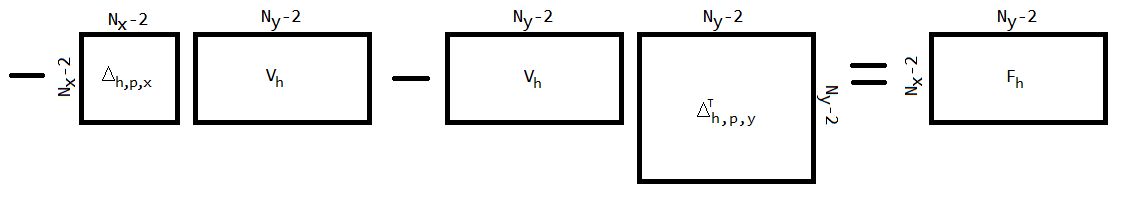
\includegraphics[width=\linewidth]{FPSExplained.png}
	\caption{}
	\label{fig:FPSexplained}
\end{figure}
\FloatBarrier
Този тип запис на задачата \rf{PoissonEq} е разгледан от Том Личи в \cite{ref34}, където областта е квадратна $L_x = L_y$ и са използвани симетрични крайни разлики от втори ред $p=2$ с нулево гранично условие в $\partial \Omega_h$. При $p=2$ операторите $\Delta_{h,2,x}$ и $\Delta_{h,2,y}$ са симетрични, което допълнително улеснява търсенето на решение на поставената задача. Настоящата глава се явява разширение на горепосочения труд при произволна правоъгълна област $2L_x \times 2L_y$ и несиметрични крайни разлики по границата на областта, където се прилага нулево гранично условие. Т.е. в общия случай матриците $\Delta_{h,p,x}$ и $\Delta_{h,p,y}$ не са симетрични както е описано в настоящата работа в глава ``Нулево гранично условие'' при $p>2$. Нека за матриците $(\Delta_{h,p,x})^T$ и $(\Delta_{h,p,y})^T$ имаме следните собствени стойности $\lambda_{x,i}$, $\lambda_{y,j}$ и собствени вектори $s_{x,i}$, $s_{y,j}$:
\begin{align}
S_x:=[s_{x,1},..,s_{x,N_x-2}],\\
D_x:= diag(\lambda_{x,1},..,\lambda_{x,N_x-2}),\\
S_y:=[s_{y,1},..,s_{y,N_y-2}],\\
D_y:= diag(\lambda_{x,1},..,\lambda_{x,N_y-2}).
\end{align}
Така се получава, че
\begin{align}\label{eigIdentity}
(\Delta_{h,p,x})^T  * S_x = S_x * D_x\nonumber\\
(\Delta_{h,p,y})^T  * S_y = S_y * D_y,
\end{align}
където $S_x, S_y$ се явяват матриците със собствените вектори и $D_x, D_y$ са диагоналните матрици със собствените стойности съответно на $(\Delta_{h,p,x})^T, (\Delta_{h,p,y})^T$. Ако положим
\be\label{subst}
X_h := ( S_x^T * V_h * S_y ) \in \RR^{(N_x-2)\times(N_y-2)},
\ee
и заместим в \rf{PsnDiscret}, се получава:
\be
-\Delta_{h,p,x} * (S_x^T)^{-1} *X_h * S_y^{-1}  -(S_x^T)^{-1} *X_h * S_y^{-1} * (\Delta_{h,p,y})^T = F_h.
\ee
Умножаваме от ляво и дясно с $ S_x^T * ( . ) * S_y$:
\be\label{fpp1}
- S_x^T *\Delta_{h,p,x} *(S_x^T)^{-1} *X_h -X_h * S_y^{-1} * \Delta_{h,p,x}^T * S_y = S_x^T * ( F_h ) * S_y.
\ee
Изразът $S_x^T * \Delta_{h,p,x}$ има следното представяне
\be
S_x^T * \Delta_{h,p,x} = (\Delta_{h,p,x}^T * S_x)^T =^{\rf{eigIdentity}} (S_x * D_x)^T = D_x * S_x^T
\ee
Последното се замества в \rf{fpp1} и използвайки пак \rf{eigIdentity}
\be\label{fpp2}
- D_x * S_x^T *(S_x^T)^{-1} *X_h  -X_h * S_y^{-1} * S_y * D_y = S_x^T * F_h  * S_y,
\ee
което след опростяване е:
\be\label{fpp2}
- D_x * X_h -X_h * D_y = S_x^T * F_h * S_y.
\ee
Уравнение \rf{fpp2} е еквивалентно на
\be\label{fpp3}
-X_{i,j} \lambda_{x,i} - \lambda_{y,j} X_{i,j} = b_{i,j}.
\ee
разписано по компоненти и така се получава, че
\be\label{fpp4}
X_{i,j} = - b_{i,j}/(\lambda_{x,i} + \lambda_{y,j} ),
\ee
където $X_h = (X_{i,j})$ и $S_y^T * F_h  * S_x = (b_{i,j})$ и това важи за всяко $(i,j)$:
$$i = 1,..,N_x-2, \quad j = 1,..,N_y-2 $$
с уточнението че $i = 0,N_x-1$, $j = 0,N_y-1$ са граничните стойности които не присъстват експлицитно в уравненията, но са взети в предвид. Имайки $X_h$ лесно може да получим $V_h$  с обратната субституция на \rf{subst}, която е 
\be\label{substInv}
V_h = (S_x^T)^{-1} * X_h * S_y^{-1}.
\ee

Важно е също да се обърне внимание и на следната задача:
\be\label{PoissonEqExt}
v-\Delta v = f,
\ee
дефинирана в областта $\Omega$ с хомогенни гранични условия $v \big|_{\partial\Omega} = 0$. В този случай дискретната версия на \rf{PoissonEqExt} използвайки \rf{DeltaH} има вида:
\be\label{PsnDiscretExt}
V_h - \Delta_{h,p,x} * V_h - V_h * (\Delta_{h,p,y}) ^{T}  = F_h,
\ee
което е аналогично с \rf{PsnDiscret} и дефинициите заложени там. Използвайки същите съждения от \rf{subst}-\rf{fpp4} лесно се получава, че:
\be\label{fpp4Ext}
X_{i,j} = - b_{i,j}/(\lambda_{x,i}  + \lambda_{x,j} -1)
\ee
за всяко $(i,j)$, $i = 1,..,N_x-2$, $j = 1,..,N_y-2 $.
\subsection{Изчислителната сложност}
Изчислителната сложност при обръщането на оператора на Лаплас изложен тук се разделя на две части. Първата част (I) е свързана с изчисляването на собствените стойности $D_x, D_y$ и вектори $S_x, S_y$ на двете матрици $(\Delta_{h,p,x})^T$ и $(\Delta_{h,p,y})^T$. Също така се включват и пресмятанията необходими за получаването на обратните матрици $(S_x^T)^{-1}$ и $S_y^{-1}$. Сложността на тези две процедури се оценя на $O(N_x^3+N_y^3)$ (\cite{ref260}) и съответно на $O(N_x^{2.37}+N_y^{2.37})$ (\cite{ref27}). Втората част (II) е предимно свързана с умножение на не-разредени матрици в дясната част на \rf{fpp2} и обратната субституция \rf{substInv}, като и в двата случая произведението се формира от три матрици  с големини както следва: първата - $(N_x-2) \times (N_x-2)$, втората (средната) - $(N_x-2) \times (N_y-2)$ и третата - $(N_y-2) \times (N_y-2)$. Това води до изчислителна сложност от 
\be\label{fpsComplex}
O(N_x N_y \bar{\epsilon}),
\ee
където $\bar{\epsilon} \in (0, max(N_x, N_y))$ (\cite{ref26, ref27}). В случая, когато областта е квадратна $N_x = N_y$ се получава че $\bar{\epsilon} = 0.37 N_x$, т.е. алгоритмичната сложност е $O(N_x^{2.37})$. При метода на Тейлор изчисленията описани в (I) се правят еднократно и получените резултати се използват в частта (II), която се прави за всеки слой по времето, т.е. (II) и \rf{fpsComplex} са с по-голяма тежест. 

\subsection{Сравнение на изчислителната сложност с факторизация на Холески}
Равенствата\rf{PsnDiscret} и \rf{PsnDiscretExt} използват матрици не по големи от $max(N_x, N_y) \times max(N_x, N_y))$, което позволява една компактност относно компютърната памет. В противен случай, ако се се борави с едномерен вектор за неизвестната функция $u$ от типа $\bar {b}_{(j-1)N_x + i} := u_{i,j}$, то тогава дискретния оператор на Лаплас ще е матрица с големина $\RR^{N_x^2 N_y^2}$ и при обръщането ѝ $-\Delta_{h,p}^{-1}\bar {b}$ посредством факторизация на Холески ще изисква изчислителна сложност от минимум $O(N_x^2 N_y^2)$ операции възползвайки се от лентовата ѝ структура. Тук напомняме, че стандартната операция по факторизация на Холески за не-разредена (пълна) матрица с големина $\RR^{N_x^2 N_y^2}$ отнема $O(N_x^3 N_y^3)$ операции.

\section{Формулировка на елиптичната задача}
Посредством смяната на променливите $x=\sqrt\beta_1 { \overline x}$, $y=\sqrt\beta_1 { \overline y}$, $U(x,y)= v({ \overline x},{ \overline y} )$ уравнение 
\rf{eq2} добива следната форма
 \begin{align}\label{eq3}
&c^2 \beta (E- \Delta) v_{{\overline y}{\overline y}} = \beta \Delta v - \Delta^2 v - \beta \Delta f(v), \\ 
&v(\overline x, \overline y) \rightarrow 0,  \Delta v(\overline x, \overline y) \rightarrow 0 ,  \quad \text{за}  \sqrt{\overline x^2 + \overline y^2} \rightarrow \infty, \nonumber
\end{align}
взимайки предвид граничното условие от \rf{eq1} и $\beta = \beta_1 / \beta_2$.
Решението $v$ на \rf{eq3} заедно с неговите производни клони към нула, когато $|{\overline x}^2 +{\overline y}^2|\rightarrow \infty$.
Навсякъде по-надолу в текста ще се използват отново старите означения $x,y$ вместо ${\overline x},{\overline y}$.

Уравнението \rf{eq3} е елиптично от четвърти ред, (а линейните втори производни в \rf{eq3} образуват елиптично уравнение от втори ред) когато е изпълнено условието $c < \min (1/ \sqrt{\beta},1)$. В настоящата работа се разглеждат единствено такива параметри $\beta$ и $c$, които удовлетворяват последното изискване.
Равенството \rf{eq3} може да се преобразува в система от две елиптични уравнения от втори ред по различни начини. Очаквайки, че производните $v_{xx}$ по оста $x$ ще са по-малки по абсолютна стойност от производните $v_{yy}$ по $y$ оста (тъй като решението се движи по $y$), заместваме $v_{yy} = \Delta v- v_{xx}$ в \rf{eq3}. След като се добави допълнителна функция $w$, се получава система еквивалентна на \rf{eq3}
\begin{equation}\label{eq4}
- (1- c^2 \beta) v_{yy} - v_{xx} + \beta (1-c^2) v - \alpha \beta v^2 = w, 
\end{equation}
\begin{equation}\label{eq44}
 - \Delta w = c^2 \beta v_{xx}. 
\end{equation}
Търсят се ненулеви решения на \rf{eq4},\rf{eq44} както е описано в \cite{ref116, ref117}: фиксира се стойността на нейзвестната функция $v$ в нулата, $v(0,0)=\theta$ и се въвеждат две нови функции: $\widehat{v}=v/{\theta} $ и $\widehat{w}=w/{\theta} $. Следователно $\widehat{v}(0,0)=1$ и 
\begin{equation}\label{eq45}
\begin{split}
 &- (1 - c^2 \beta) \widehat{v}_{yy} -\widehat{v}_{xx} + \beta (1-c^2) \widehat{v} - \alpha \beta \theta \widehat{v}^2 = \widehat{w}, \\
 &- \Delta \widehat{w} =  c^2 \beta \widehat{v}_{xx}.
\end{split}
\end{equation}
Стойността на $\theta$ се намира използвайки следната зависимост
\begin{equation}\label{eqtheta}
\theta = \frac{ (1-c^2 \beta) \widehat{v}_{yy} + \widehat{v}_{xx} - \beta (1-c^2) \widehat{v} +\widehat{w}}{\alpha \beta \widehat{v}^2 } |_{x=0,y=0}.
\end{equation}
Численото решение на уравнение \rf{eq45} се намира чрез метода на простата итерация като изкуствено се добавят производни по времето както следва:
\begin{align}\label{eq5}
\begin{split}
 &\frac {\partial \widehat{v}}{\partial t} - (1 - c^2 \beta) \widehat{v}_{yy} -\widehat{v}_{xx} + \beta (1-c^2) \widehat{v} - \alpha \beta \theta \widehat{v}^2 = \widehat{w}, \\
 &\frac {\partial \widehat{w}}{\partial t} - \Delta \widehat{w} =  c^2 \beta \widehat{v}_{xx}. 
\end{split}
\end{align}
По този начин стационарната системата от двете уравнения \rf{eq45} се заменя с преходните във времето уравнения дефинирани в \rf{eq5} с условието, че решенията $\widehat{v}$ и $\widehat{w}$ схождат линейно спрямо времето към решенията на \rf{eq45}.

\section{``Метод на простата итерация'' при елиптичната задача}
Поради симетрията на проблема ще се разглеждат решенията получени само в първи квадрант $\omega = [0,L_x] \times[0,L_y] \in \Omega$. Дискретизацията на тази област води до мрежата $\omega_h$ дефинирана по следния начин:
$$
\omega_h = \{(x_i,y_j): x_i = ih, y_j = jh, i = 0,\cdots ,(N_x-1)/2, j = 0,\cdots , (N_y-1)/2 \},
$$
където дискретната стъпка $h$ е същата както при $\Omega_h$ и $\omega_h \in \Omega_h$. Времевата област е дефинирана чрез интервала $[0, \widehat T]$ или просто $\widehat T$, където стъпката по времето $\tau$ варира в зависимост от големината на остатъка на решението. Това спомага за автоматизиране контрола върху грешката (от апроксимацията и изчисленията, но с условието че итеративният Метод на простата итерация е сходящ). Стойността на функцията $v$ в точка от мрежата $x_i,y_j,t_k$ е означена с $v_{i,j}^{(k)}$. 
Дискретизацията на пространствените производни в \rf{eq5} е направена посредством централните крайни разлики дефинирани в \rf{fdx}, \rf{fdy} и описани в \rf{table:A00}. Грешката от апроксимацията при формули \rf{fdx} и \rf{fdy} е $O(h^p)$. Замествайки оператора на Лаплас в \rf{eq5} с дискретния Лапласиан $\Delta_{h,p} (v_{i,j}) = (v_{i,j})_{\widehat{xx},p} + (v_{i,j})_{\widehat{yy},p}$ се получават крайни разлики с до шести ред на апроксимация (във вътрешността на областта $\omega_h$). Това води до по-висок ред на сходимост за използваните методи при достатъчно гладки решения. По този начин се получават по-точни решения върху по-едра мрежа. 
\par
Явното правилото на Ойлер е използвано за апроксимацията на нововъведените производни по времето. Нелинейните членове в \rf{eq3} се пресмятат на $t^{(k)}$ слой по времето. Така, численото решение в $t^{(k+1)}$ слой по времето е пресметнато директно чрез численото решение от предходния слой $t^{(k)}$:
\begin{equation}\label{eq55}
\begin{split}
&\frac {\widehat{v}_{i,j}^{(k+1)}-\widehat{v}_{i,j}^{(k)}}{\tau}- (1-c^2 \beta) \widehat{v}_{i,j,{\widehat{yy},p}}^{(k)} - \widehat{v}_{i,j,{\widehat{xx},p}}^{(k)} + \beta (1-c^2 ) \widehat{v}_{i,j}^{(k)} - \alpha \beta \theta (\widehat{v}_{i,j}^{(k)})^2 = \widehat{w}_{i,j}^{(k)}, \\
&\frac  {\widehat{w}_{i,j}^{(k+1)} -\widehat{w}_{i,j}^{(k)}} {\tau} - \Delta_{h,p} \widehat{w}_{i,j}^{(k)} =  c^2 \beta \widehat{v}_{i,j,{\widehat{xx},p}}^{(k)}.
\end{split}
\end{equation}
Този метод за решаване на уравненията \rf{eq45} е известен в литературата още като "Метод на простата итерация" при линейни и нелинейни уравнения \cite{sam}. С помощта на матриците $\Delta_{h,p,s,x}$ и $\Delta_{h,p,s,y}$ прилагаме нулево и симетрично гранични условия по границите на областта $\partial \omega$ запазвайки реда на използваната апроксимация $O(h^p)$ в \rf{eq55}. Така отчитайки \rf{PsnDiscretSym} се получава следното матрично уравнение допълващо \rf{eq55} отчитайки всички точки в $\omega_h$:
\begin{equation}\label{eq555}
\begin{split}
\frac {\widehat{v}^{(k+1)}-\widehat{v}^{(k)}}{\tau}- (1-c^2 \beta) \widehat{v}^{(k)} * (\Delta_{h,p,s,y})^T - \quad\quad\quad\;&\\
-\Delta_{h,p,s,x} * \widehat{v}^{(k)}+ \beta (1-c^2 ) \widehat{v}^{(k)} - \beta \theta f(\widehat{v}^{(k)}) &= \widehat{w}^{(k)}, \\
\frac  {\widehat{w}^{(k+1)} -\widehat{w}^{(k)}} {\tau} - \Delta_{h,p,s,x} * \widehat{w}^{(k)} - \widehat{w}^{(k)} * (\Delta_{h,p,s,y})^T &=  c^2 \beta \Delta_{h,p,s,x} * \widehat{v}^{(k)},
\end{split}
\end{equation}
където $\widehat{v}^{(k)}, \widehat{w}^{(k)}, \widehat{v}^{(k+1)}, \widehat{w}^{(k+1)} \in \RR^{(N_x-1)/2 \times (N_y-1)/2}$ са матрици съответно с елементи ${v}_{i,j}^{(k)}$, ${w}_{i,j}^{(k)}$, ${v}_{i,j}^{(k+1)}$ и ${w}_{i,j}^{(k+1)}$.
\subsection{Начални данни}
 Цикличната процедура описана в \rf{eq55} се нуждае от начални стойности за функиите $\widehat{v},\widehat{w}$, които са взети от "best-fit" формулите в \cite{Ch2011}. 
Решението от задачата \rf{eq3} при $c=0$ също е добро приближение и служи на начални стойности на \rf{eq55} при скорости близки до допустимия максимум $c \approx \min (1/ \sqrt{\beta},1)$, $c < \min (1/ \sqrt{\beta},1)$. При $c=0$ уравнение \rf{eq3} добива следния вид:
\be\label{eq3c0}
\Delta (\beta  v - \Delta v - \beta f(v)) = 0.
\ee
В частност, ако за уравнението 
\be\label{eq3c01}
\beta v - \Delta v - \beta f(v) = 0
\ee
съществува решение $\nu$, то също ще удовлетворява и \rf{eq3c0}. Ако разгледаме само радиално симетрични решения на \rf{eq3c01} и преминем в полярни координати получаваме:
\begin{align}\label{eq3c02}
\beta v_{polar}(r)  - \frac{ \partial^2 v_{polar} } {\partial r^2}(r) - \frac{1}{r} \frac{ \partial v_{polar} } {\partial r}(r)  - \beta f(v_{polar}(r)) = 0, \nonumber \\
\frac{ \partial v_{polar} } {\partial r}(0) = 0, \quad v_{polar}(r) \rightarrow 0, \; \text{as} \; r \rightarrow \infty
\end{align}
Последното диференциално уравнение и числените му решения са разгледани в \cite{ref1c0, ref2c0}.

\subsection{Контрол на стъпката по времето}
Възможно е да се използва нефиксирана стъпка по времето $\tau$ за оптимизиране скоростта на сходимост. Когато $\tau > \tau_{stab}$ премине условието за устойчивост, решението започва да разхожда и става назъбено. Тези знаци се проявяват първоначално при остатъка \rf{residual}, докато численото решение $u$ е все още монотонно и разликите между две последователни итерации не са големи. Когато последното се случи, произволно сечение на остатъка $R$ се описва с дискретна функция сменяща положителни с отрицателни стойности върху мрежата. Това е ясен знак, че стъпката $\tau$ трябва да се намали, в противен случай се увеличава. Промяната се случва на всяка итерация с фактор $f_{\tau} \in \{0.72, 1.015\}$, където $\tau_{new} := f_{\tau}\tau$.

Самият остатък $R^{(k)}_{i,j}$ от дискретната апроксимация на \rf{eq3} в произволна точка от мрежата $(x_i,y_j,t^{(k)})$ е дефиниран чрез:
\begin{equation}\label{residual}
R_{i,j}^{(k)} := 
c^2\beta (\widehat{v}^{(k)}_{i,j})_{\widehat{yy},p} + \Delta_{h,p}(-\beta \widehat{v}^{(k)}_{i,j} - c^2\beta (\widehat{v}^{(k)}_{i,j})_{\widehat{yy},p} + \Delta_{h,p} \widehat{v}^{(k)}_{i,j} 
+ \alpha \beta \theta (\widehat{v}^{(k)}_{i,j})^2  ).
\end{equation}
Последната дефиниция може да се запише в матричен вид използвайки $\Delta_{h,p,s,y}$ и $\Delta_{h,p,s,y}$:
\begin{align}\label{residualM}
&R^{(k)} = 
c^2\beta \widehat{v}^{(k)}*(\Delta_{h,p,s,y})^T + \Delta_{h,p,s,x} * \widehat{z}^{(k)} + \widehat{z}^{(k)} * (\Delta_{h,p,s,y} )^T, \nonumber\\
&\widehat{z}^{(k)}  = \nonumber\\
&-\beta \widehat{v}^{(k)} - c^2\beta \widehat{v}^{(k)}*(\Delta_{h,p,s,y})^T + \Delta_{h,p,s,x} * \widehat{v}^{(k)} +  \widehat{v}^{(k)} * (\Delta_{h,p,s,y})^T 
+ \beta \theta f(\widehat{v}^{(k)}).
\end{align}
 
\subsection{Критерии за спиране}
Стандартният критерии за спиране на итеративния Метод на простата итерация от уравнения \rf{eq55} е когато разликата между две последователни решения стане достатъчно малка
\begin{equation*}
\Vert \widehat{v}^{(k+1)}-\widehat{v}^{(k)}\Vert  < \epsilon \Vert \widehat{v}^{(k)}\Vert ,
\end{equation*}
при предварително избрани подходяща норма и достатъчно малък праг $\epsilon$. В конкретния случай са избрани $L_1$ нормата (понеже има ниска изчислителна сложност) и $\epsilon < 1\times10^{-6}$:
\begin{equation}\label{crit1}
\max_{i,j} |\widehat{v}^{(k+1)}_{i,j}-\widehat{v}^{(k)}_{i,j}| < 1\times10^{-6} \max_{i,j} |\widehat{v}^{(k)}_{i,j}|.
\end{equation}
Критерият за спиране може допълнително да се разшири и да изпълнява още едно условие, което ще го направи по-стриктен. Нека остатъкът $R_{i,j}^{(k)}$ от \rf{residual} да изпълнява следната зависимост
\begin{equation}\label{crit2}
\max_{i,j} |R_{i,j}^{(k)}| < \epsilon = 1\times10^{-6}.
\end{equation}
Така критерият за спиране се определя, когато двете неравенства \rf{crit1} и \rf{crit2} са едновременно изпълнени.
\subsection{Метод на простата итерация - алгоритмични стъпки}
Следващия запис дефинира основните стъпки при числената имплементация на метода на простата итерация.
\\
1)Препроцесор - зареждат се началните данни $(v^0, w^0)$ върху мрежата $\omega_h$.  Задават се началната стъпка по фиктивното време $\tau$ както и прагът $\epsilon$.
\\
2) Процесор $(k \rightarrow k+1)$. На всяка стъпка по времето се изчисляват: 
\par
2.1) максимума на решението $\theta_k$ в $(0,0)$  от дискретното уравнение \rf{eqtheta},
\par
2.3) следните изрази, които са части от дискретният оператор на Лаплас приложен върху $\widehat{v}^{(k)}$ и $\widehat{w}^{(k)}$
\begin{align}\label{helper}
\Delta_{h,p,s,x} * \widehat{v}^{(k)}, \quad \widehat{v}^{(k)} * (\Delta_{h,p,s,y})^T, \nonumber\\
\Delta_{h,p,s,x} * \widehat{w}^{(k)},\quad  \widehat{w}^{(k)} * (\Delta_{h,p,s,y})^T,
\end{align}
\par
2.4) търсените функции $(\widehat{v}^{(k+1)}, \widehat{w}^{(k+1)})$  на следващия слой по времето $t^{(k+1)}$ посредством явната схема на Ойлер \rf{eq555} и вече изчислените изрази в \rf{helper},
\par
2.5) остатъкът $R^{(k+1)}_{i,j}$ от \rf{residual} използвайки \rf{helper},
\par
2.6) критериите за спиране  \rf{crit1} и \rf{crit2} и съответната проверка заложена в тях,
\par
2.6) новата стъпка по времето $\tau$. Записва се $t^{(k+1)}=t^{(k)}+\tau$.

Сложността на алгоритъма зависи от матричните умножения в \rf{eq555} и \rf{residualM} с матриците $\Delta_{h,p,s,x}$ и $\Delta_{h,p,s,y}$, които имат лентова структура. Този тип изчисления могат да се извършат с $O(n_z^2)$ операции, където $n_z = max\{(N_x-1)/2, (N_y-1)/2\}$.  Добавяйки и итерациите по фиктивното време $n_t$ се получава следната изчислителна сложност:
\be\label{complexElpt}
O(n_z^2 n_t).
\ee
Множеството изчислителни тестове показват, че за задачата \rf{eq555} и избраният праг $\epsilon = 1 \times 10^9$, числото $n_t$ е съизмеримо с големината на областта $\omega_h$
\be
n_t \approx \frac{N_x-1}{2} \frac{N_y-1}{2}.
\ee

\section{Ред на сходимост при ``метода на простата итерация''}\label{validation}
В тази част са показани числени резултати от елиптичната задача \rf{eq3} и приложеният за нея ``Метод на простата итерация''. Използваните крайни разлики и параметри $c$, $\alpha$, $\beta$, както и стъпките по пространството са описани в Таблица \rf{tableP}. Приложеният дискретен оператор на Лаплас е подробно дефиниран в секцията ``Симетрично гранично условие по абцисата и ординатата при елиптичната задача''.

\begin{table}[ht]
\centering
		\begin{tabular}{||c|l|ll|ll||}
			\hline
			\hline
      \multirow{2  }{*}{FDS}        & \multirow{2  }{*}{$h$, $\tau$}  &  	\multirow{2  }{*}{ $\Vert \bar{ E_i} \Vert_{L_2}$ }	&Ред на	& \multirow{2  }{*}{ $\Vert \bar{ E_i} \Vert_{L_\infty}$ } 		&Ред на   \\
	                                        &                                                & 							 					&  сход. 	& 								       					& сход. \\
   					\hline 
					\hline 
$\beta = 3$   	&0.2    										&            &            &           &   \\
      c=0.45 	&0.1    & 0.014232  						&            & 0.016732 			&   \\
   $O(h^2)$     &0.05   & 0.003238  						&2.14  & 0.003997					& 2.07 \\
\hline 
$\beta = 3$   	&0.2   &            &            &             &    \\
      $c=0.45 $ &0.1   &   0.001758   &           &  0.002499  &   \\
       $O(h^4)$	&0.05  &  0.000114 & 3.95    & 0.000168  & 3.90  \\
\hline
$\beta = 3$   	&0.2   &            &        &                  &      \\
   $c=0.45$   	&0.1   &  3.6184e-04 &           & 5.9054e-04      &       \\
     $O(h^6)$	&0.05  &  1.1680e-05  & 4.95  & 1.1690e-05 & 5.66         \\
			\hline
			\hline 	
$\beta = 1$   	&0.4   &             &           &                & \\
     $c=0.9$     &0.2   &  0.043898  &             & 0.017906      &    \\
     $O(h^2)$	&0.1  & 0.009999 & 2.13       & 0.004348      & 2.04  \\
\hline 	
 $\beta = 1$   	&0.4  &            &               &               &     \\
     $c=0.9$  	&0.2   & 0.006309  &              & 0.002965      &        \\
     $O(h^4)$	&0.1  &  0.000432 &3.87        & 0.000200 &  3.89        \\
    \hline
 $\beta = 1$	&0.4   &             &        &               &        \\
   $ c=0.9$  	&0.2   &  0.001285  &        &0.000671     &       \\
       $O(h^6)$	&0.1  &   0.000132 &3.28  & 0.000029 &   4.52       \\
	   \hline
			\hline 
		\end{tabular}
		\caption{Ред на сходимост при Метода на простата итерация с апроксимации $O(h^{2})$, $O(h^{4})$ и $O(h^{6})$ за Тест  1 и Тест 2. Грешките $E_i$ са пресметнати в $L_2$ и $L_\infty$ норми.}
\label{tab:a}
\end{table}
\FloatBarrier
Таблица \rf{tab:a} показва скоростта на сходимост при изчисление на решението от диференчното уравнение \rf{eq555} за апроксимациите $O(h^{2})$, $O(h^{4})$ and $O(h^{6})$ описани в първата колона. Втората колона дефинира използваната стъпката по пространството. Третата и четвъртата колона показват грешките от апроксимациите $E_i$ и скоростите на сходимост получени посредством правилото на Рунге \rf{Runge} върху три вложени мрежи. С увеличаването на степента на апроксимация $p=2,4,6$, грешките $E_i$ намаляват, което води до по-прецизни решения. При $p=6$ и двата числени теста постигат по-нисък резултат за сходимостта от очакваното. Най-ясно изразен е случаят от Тест 2 и $p=6$, при които сходимостта в $L_2$ норма е $3.28$. Стойностите на непрекъснатото решение са все още достатъчно големи в пограничните райони $x=L_x$, $y=L_y$ и оказват влияние върху сходимостта. За целта е необходимо да се разгледа численото решение върху по-голяма област или да се приложи подходящо гранично условие.  При Тест 2 вълната е с по-голяма дисперсия както се вижда от картинките на Фигура \ref{fig:solutions} и вълната заема по голям обем в пограничните райони. Въпреки повече от два пъти по-голямата дължина $L_y$ в Тест 2, стойността на функцията $\widehat v$ в $y=58$ е по-голяма от тази при Тест 1 както е показано на Фигура \ref{profilesOnBnd}. Затова резултатите от сходимостта при Тест 2 - $3.28$, $4.52$ в $L_2$ и $L_\infty$ норми са по-лоши спрямо Тест 1 - $4.95$, $5.66$ в $L_2$ и $L_\infty$ норми. Впоследствие ще бъдат разгледани и резултати за сходимостта на ``метода на простата итерация'' използвайки правилото на Рунге \ref{Runge} с приложено ненулево гранично условие.
\begin{figure}[ht]
	\begin{minipage}[b]{0.5\linewidth}
		\raggedleft
		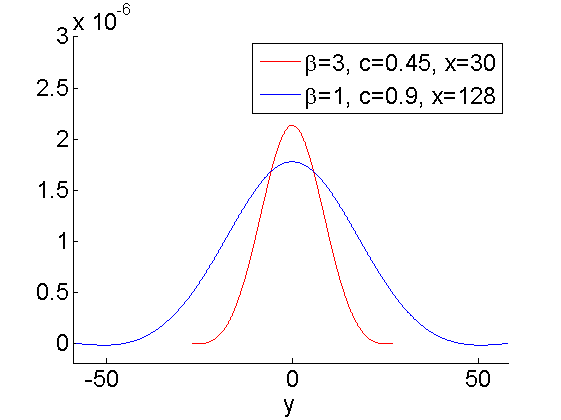
\includegraphics[width=\linewidth]{SolutionView/ChristovIC_128vsChristov_30on_xEnd.png}
	\end{minipage}	
	\begin{minipage}[b]{0.5\linewidth}
		\raggedright
		 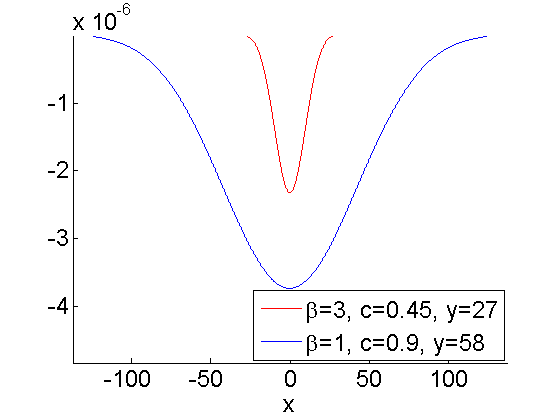
\includegraphics[width=\linewidth]{SolutionView/ChristovIC_128vsChristov_30on_yEnd.png}
	\end{minipage}
	\caption{Сечения на численото решение при Тест 1 ($\beta=3, c=0.45$) и Тест 2 ($\beta=1, c=0.90$) в края на областта $\partial \Omega_h$:  $x=30$ за Тест 1 и $x=128$ за Тест 2 (левия панел);  $y=27$ за Тест 1 и $y=58$ за Тест 2 (десния панел).}
	\label{profilesOnBnd}
\end{figure}
\FloatBarrier
\begin{figure}[ht]
	\begin{minipage}[b]{0.5\linewidth}
		\raggedleft
		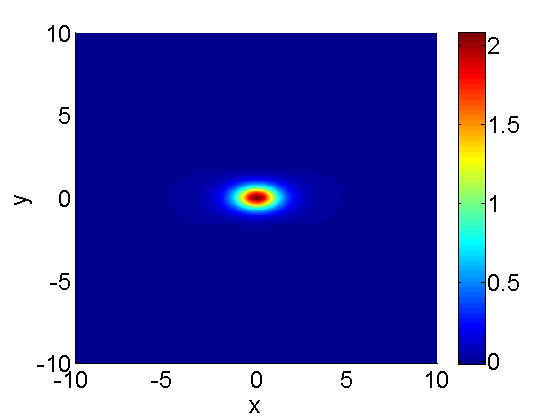
\includegraphics[width=\linewidth]{SolutionView/ChristovIC_30_bt3_c045_topview.png}
	\end{minipage}
	\begin{minipage}[b]{0.5\linewidth}
		\raggedright
		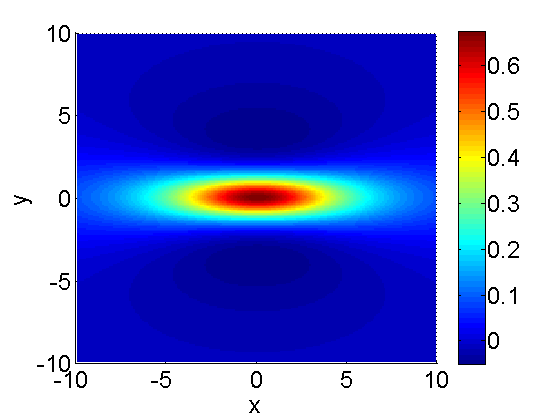
\includegraphics[width=\linewidth]{SolutionView/ChristovIC_128_bt1_c090_topview.png}
	\end{minipage}
	\begin{minipage}[b]{0.5\linewidth}
		 \raggedleft
		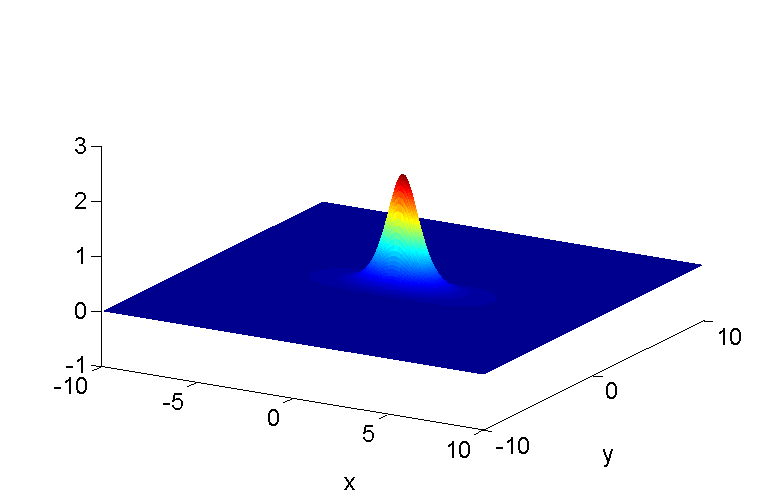
\includegraphics[width=\linewidth]{SolutionView/ChristovIC_30_bt3_c045_prpview.png}		
		\centerline{$\beta = 3$, $c = 0.45$ }
	\end{minipage}
	\begin{minipage}[b]{0.5\linewidth}
		 \raggedright
		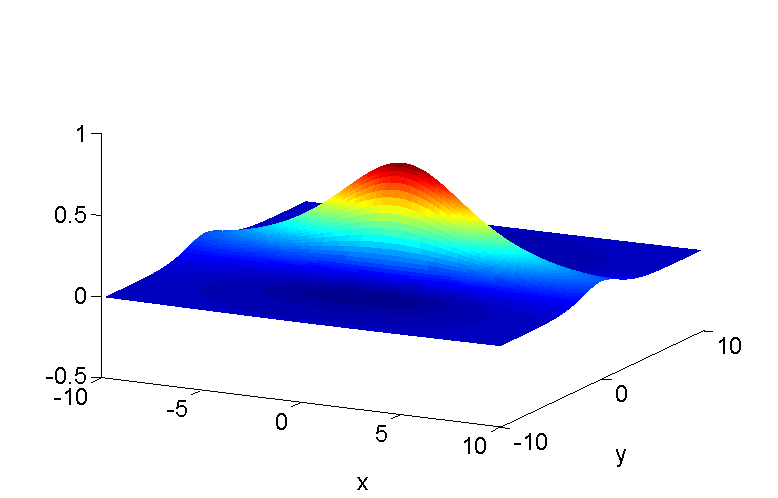
\includegraphics[width=\linewidth]{SolutionView/ChristovIC_128_bt1_c090_prpview.png}
		\centerline{$\beta = 1$, $c = 0.9$}
	\end{minipage}
	\caption{2Д и 3Д профили на численото решение $\widehat v$ от \rf{eqtheta} и \rf{eq555}. За изображенията са избрани най-ситните стъпки - $h=0.05$ (ляво), $h=0.1$ (дясно) .}
	\label{fig:solutions}
\end{figure}
\section{Числени резултати от ``метода на простата итерация''}\label{results}
В тази част са представени резултатите от приложения числен метод описан по-горе за елиптичното уравнение \rf{eq3}. Потвърждават се и характерните свойства на получените решения за различни стойности на параметрите $\beta$ и $c$, които са представени първоначално в \cite{ref116,Ch2011} като например зависимостта на формата на вълната от скоростта $c$ и дисперсията $\beta$ и асимптотичното поведение $\frac{1}{x^2 + y^2}$ на безкрайност. В допълнение са открити и други релации например за положителните и отрицателните области на решението.
Също така е последното е сравнено с ``best-fit'' апроксимационните формули от \cite{Ch2011}, като това сравнение е все още липсващо в литературата, но се оказва съществен елемент и повратна точка в изследването на хиперболичната задача \rf{eq1}-\rf{eq11}. Тук напомняме на читателя, че ``best-fit'' формулите са използвани за начално условие в итеративния алгоритъм.

\subsection{Остатък}

\begin{figure}[htbp]
	\begin{minipage}[b]{0.5\linewidth}
		 \centering
		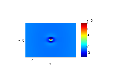
\includegraphics[width=\linewidth]{../EllipticEquationSJC/residual/residual_bt5c03.eps}
		\centerline{$\beta = 3$, $c = 0.45$}
	\end{minipage}	
	\begin{minipage}[b]{0.5\linewidth}
		\centering
		 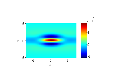
\includegraphics[width=\linewidth]{../EllipticEquationSJC/residual/residual_bt1c09.eps}
	\centerline{$\beta = 1$, $c = 0.9$ }
	\end{minipage}
		\caption{Резидуала \rf{residual} от решението от последната итерация при уравнения \rf{eq555} }
		\label{resid}
\end{figure}
\FloatBarrier
На Фигура \ref{resid} е представен остатъкът \rf{residual}, който е запазен от последната стъпка на итеративната схема \rf{eq555}, като за левия панел  параметрите са $\beta = 3$ и $c = 0.45$, а за десния $\beta = 1$ и $c = 0.9$. И в двата случая $\epsilon =1e-6$, а използваните крайни разлики са от шести порядък. Разликите в решенията между последните две итерации е $0.000e-000$ и $0.000e-000$ съответно за първия и втория пример. Така, диференчната схема \rf{eq55} е удовлетворена с голяма прецизност както от апроксимации на вторите производни с до шести ред така и от ниският праг $\epsilon =1\times10^{-6}$. От друга страна разглеждайки формулите от ``best-fit'' апроксимацията от \cite{Ch2011} се вижда, че третите, четвъртите и други производни по пространството от по висок ред са неограничени в околност на нулата $(0,0)$. Така нито елиптичното уравнение \rf{eq3}, нито остатъка \rf{residual} могат да бъдат пресметнати в класическия смисъл и следователно не са удовлетворени от ``best-fit'' формулите!

\subsection{Производни на решението}
\begin{center}
\begin{table}[ht]
\centering
		\begin{tabular}{||c|l|ll|ll||}
			\hline
			\hline
      FDS       & $h$ &errors in $L_2$&Conv. Rate& errors in $L_\infty$&Conv. Rate\\
   			\hline 
					\hline 
      c=0.45    &0.8    &             &            &           &   \\
   $O(h^2)$     &0.4    &~ 2.9698e-01  &            &~4.2497e-01 &   \\
                &0.2   &~ 6.8742e-02  &~~2.1111  &~8.6465e-02 &~~2.2972 \\
               	 \hline 
     c=0.1      &0.8   &             &           &                & \\
     $O(h^2)$   &0.4   &~ 3.4849e-01  &             &~3.0271e-01      &    \\
                &0.2  &~ 8.7696ee-02 &~~1.9905       &~7.5691e-02      &~~1.9998  \\
			\hline
			\hline 	
      c=0.45    &0.8   &            &            &             &    \\
       $O(h^6)$ &0.4   &~ 1.0766e+00   &           &~1.2316e+00  &   \\
                &0.2  &~ 3.5768e-02 &~~4.91117    &~5.8927e-02  &~~4.3855  \\
					  			\hline 	
     c=0.1      &0.8  &            &               &               &     \\
     $O(h^6)$  &0.4   &~ 8.0095e-01  &              &~9.8911e-01      &        \\
               &0.2  &~ 1.5680e-02&~~5.6747        &~2.1238e-02 &~~5.5414       \\
		   \hline
			\hline 
		\end{tabular}
		\caption{Грешките в $L_2$ и $L_\infty$ норми заедно със сходимостта на четвъртите производни по $x$ пресметнати с $O(h^2)$ и $O(h^6)$ апроксимации.}
\label{tab:fourth-der}
\end{table}
\end{center}
\FloatBarrier
Целта на този параграф е да покаже, че дискретните производни на решението от четвърти ред $v_{\widehat{xxxx}}$ схождат числено, когато стъпката $h$ намалява. За целта е приложено правилото на Рунге \rf{Runge} върху три вложени мрежи с размери $h$, $h/2$, $h/4$, а получените резултати за сходимостта $\xi$ са представени в Таблица \rf{tab:fourth-der}. В заключение се вижда, че дискретните производни $v_{\widehat{xxxx}}$ са ограничени и сходящи. Тестове със смесените производни - $v_{xxyy}$ и само по $y$ - $v_{yyyy}$ не са представени тук, но резултатите от тях са сходни като тези при $v_{xxxx}$.

\subsection{Форма на решението}

\begin{figure}[ht]
	\begin{minipage}[b]{0.5\linewidth}
		\raggedleft
		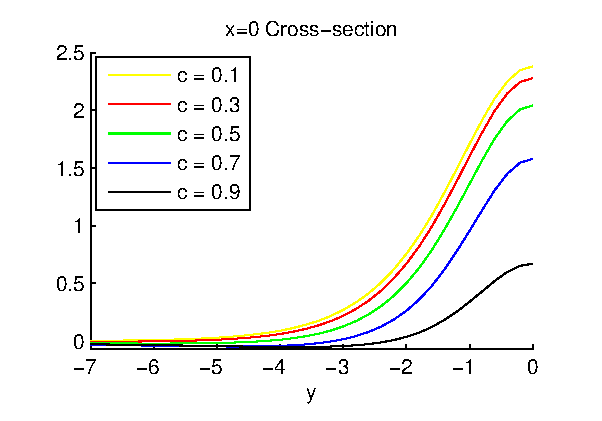
\includegraphics[width=\linewidth]{../EllipticEquationSJC/cross-sections/c=01__09beta=1x=0.eps}
	\end{minipage}	
	\begin{minipage}[b]{0.5\linewidth}
		\raggedright
		 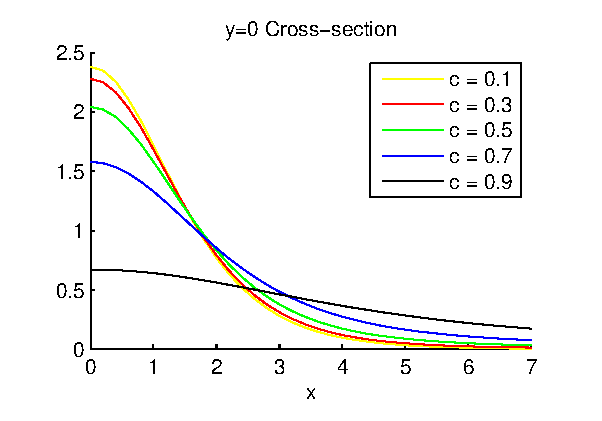
\includegraphics[width=\linewidth]{../EllipticEquationSJC/cross-sections/c=01__09beta=1y=0.eps}
	\end{minipage}
	\begin{minipage}[b]{0.5\linewidth}
		\raggedleft
		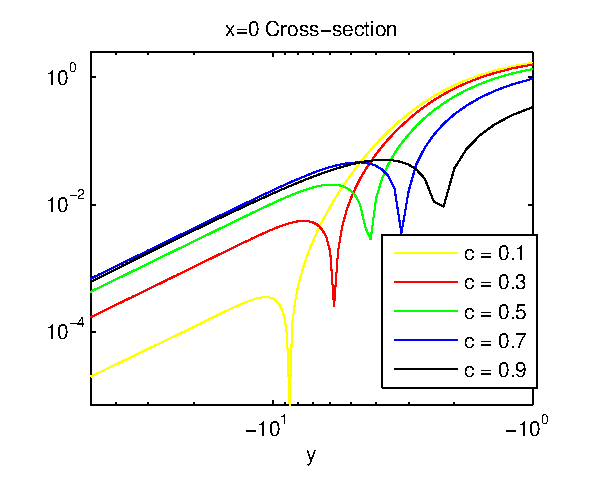
\includegraphics[width=\linewidth]{../EllipticEquationSJC/cross-sections/c=01__09beta=1Logx=0.eps}
	\end{minipage}	
	\begin{minipage}[b]{0.5\linewidth}
		\raggedright
		 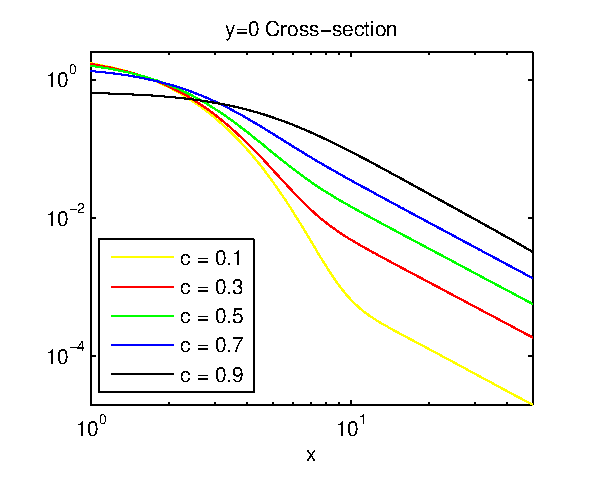
\includegraphics[width=\linewidth]{../EllipticEquationSJC/cross-sections/c=01__09beta=1Logy=0.eps}
	\end{minipage}
	\caption{Сечения на численото решение при $\beta=1$ и различни скорости $c$.}
	\label{profilesSpeedVarying}
\end{figure}
Фигура \rf{fig:solutions} показва формата на решението получено с параметрите заложени съответно в Тест 1 (ляво $c=0.45$,  $\beta=3$) и Тест 2 (дясно $c=0.9$,  $\beta=1$) при $\alpha = 1$. Показаната област в ляво е $[-5,5] \times [-5,5]$, а в дясно е $[-10,10] \times [-10,10]$. Разбира се, решението е пресметнато в правоъгълника $\omega_h$ и използвайки симетрията му е построено в цялата област $\Omega_h$, но за да изпъкне формата, която е близо до максимума, стойностите, които са по ръбовете и близки до нула, са изрязани. Вижда се, че при $\beta=1$ дисперсията на вълната е по-голяма спрямо формата получена при $\beta=3$.
Детайлно са разгледани и зависимостите на формата на вълната спрямо два от параметрите - дисперсията $\beta=\beta_1 / \beta_2$ и скоростта $c$.
Фигура \ref{profilesSpeedVarying} показва сеченията на решението при $x=0$ и $y=0$, за различни скорости $c=0.1, 0.3, 0.5, 0.7, 0.9$ при $\beta = 1$. Големината на областта е $L_x = L_y = 50$, стъпката по пространството е $h = 0.2$, а $\epsilon = 1.0e-06$. Горните две графики представят резултатите в линеен вид, докато долните две представят резултатите в логаритмични скали по $x$ и $y$. При логаритмичните панели във Фигура \rf{profilesSpeedVarying} ясно изпъква асимптотичното поведение на решението $1/x^2$ и $1/y^2$ съответно при сеченията $y=0$ и $x=0$ \cite{ref116, ref117}. Графиките показват, че с увеличаването на скоростта $c$ максимума на вълната намалява (остротата във върха се губи), заема повече обем по $x$ оста и изтънява по оста на движение $y$, както е показано в \cite{ref116, ref117}.
\begin{figure}[ht]
	\begin{minipage}[b]{0.5\linewidth}
		\raggedleft
		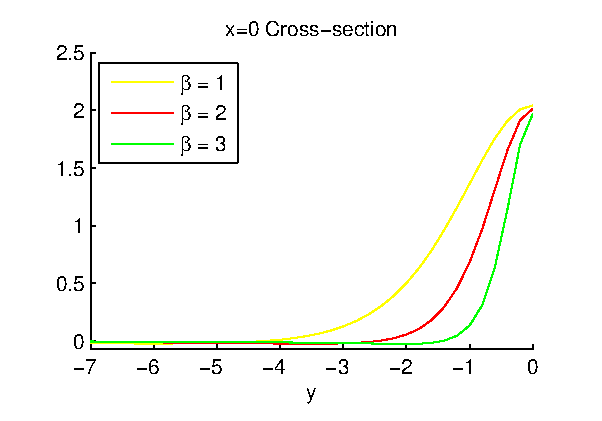
\includegraphics[width=\linewidth]{../EllipticEquationSJC/cross-sections/c=05beta=1__3x=0.eps}
	\end{minipage}	
	\begin{minipage}[b]{0.5\linewidth}
		\raggedright
		 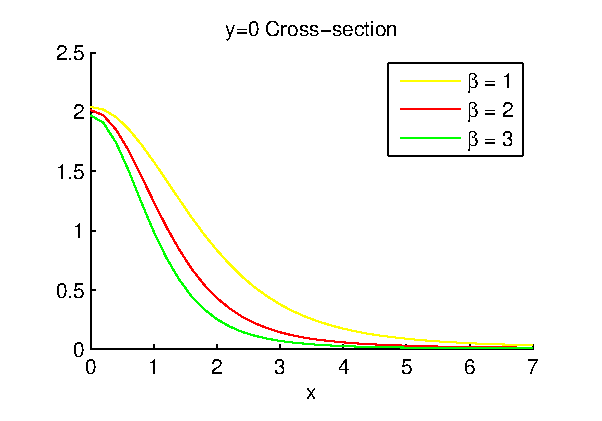
\includegraphics[width=\linewidth]{../EllipticEquationSJC/cross-sections/c=05beta=1__3y=0.eps}
	\end{minipage}
	\begin{minipage}[b]{0.5\linewidth}
		\raggedleft
		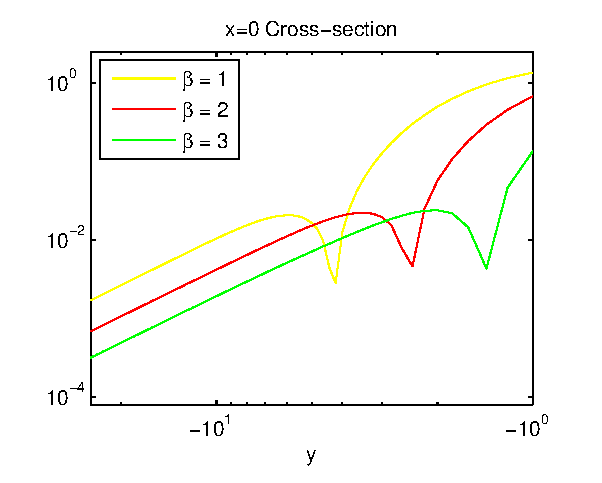
\includegraphics[width=\linewidth]{../EllipticEquationSJC/cross-sections/c=05beta=1__3Logx=0.eps}
	\end{minipage}	
	\begin{minipage}[b]{0.5\linewidth}
		\raggedright
		 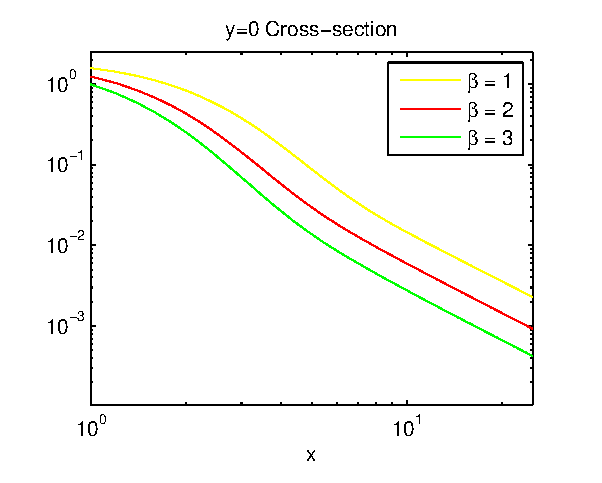
\includegraphics[width=\linewidth]{../EllipticEquationSJC/cross-sections/c=05beta=1__3Logy=0.eps}
	\end{minipage}
	\caption{Сечения на численото решение при $c=0.5$ и варираща дисперсия $\beta$.}
	\label{profilesDispVarying}
\end{figure}
Фигура \ref{profilesDispVarying} показва сеченията на решението при $x=0$ и $y=0$, за различни параметри $\beta=1, 2, 3$ при фиксирана скорост $c=0.5$. Горните две графики представят резултатите в линеен вид, докато долните две представят резултатите в логаритмични скали по $x$ и $y$. При логаритмичните панели във Фигура \rf{profilesDispVarying} отново изпъква асимптотичното поведение на решението $1/x^2$ и $1/y^2$ съответно при сеченията $y=0$ и $x=0$ \cite{ref116, ref117}. Графиките показват, че с увеличаването на дисперсионния параметър $\beta$ максимума на вълната намалява и формата ѝ изтънява по $x$ и $y$ осите (изостря се във върха), както е показано в \cite{ref116, ref117}.
\begin{figure}[htbp]
	\begin{minipage}[b]{0.48\linewidth}
		\raggedleft
		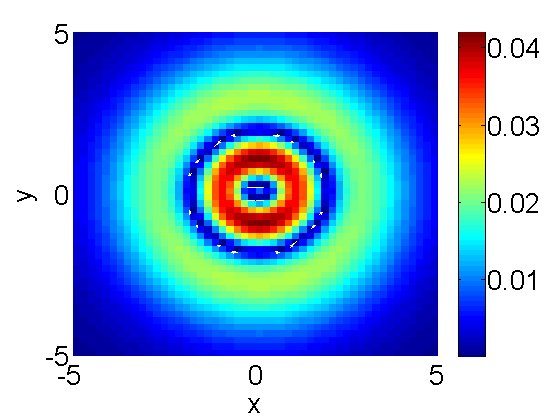
\includegraphics[width=\linewidth]{BestFitVsSimpleIter/ChristovIC_50_bt1_c017_h02_O(h^6).png}
	\end{minipage}
	\begin{minipage}[b]{0.48\linewidth}
		 \raggedright
		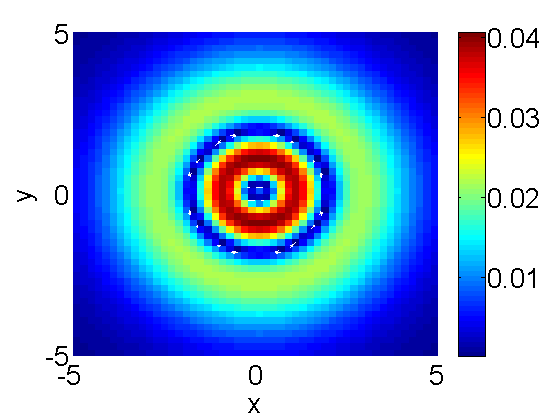
\includegraphics[width=\linewidth]{BestFitVsSimpleIter/ChristovIC_50_bt1_c010_h02_O(h^6).png}
	\end{minipage}
	\begin{minipage}[b]{0.48\linewidth}
		\raggedleft
		 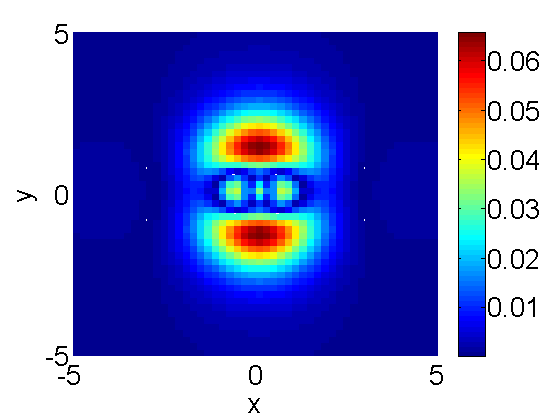
\includegraphics[width=\linewidth]{BestFitVsSimpleIter/ChristovIC_50_bt3_c017_h02_O(h^6).png}
	\end{minipage}
	\begin{minipage}[b]{0.48\linewidth}
		\raggedright
		 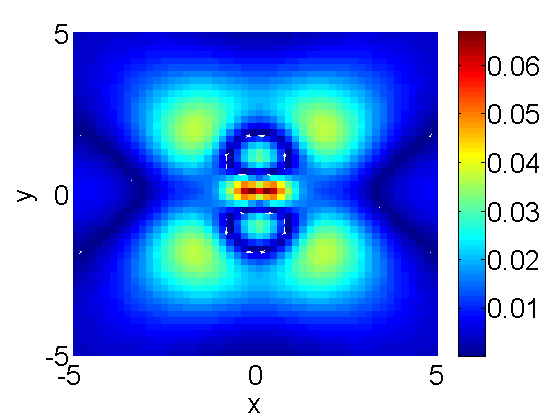
\includegraphics[width=\linewidth]{BestFitVsSimpleIter/ChristovIC_50_bt1_c050_h02_O(h^6).png}
	\end{minipage}
	\begin{minipage}[b]{0.48\linewidth}
		\raggedleft
		 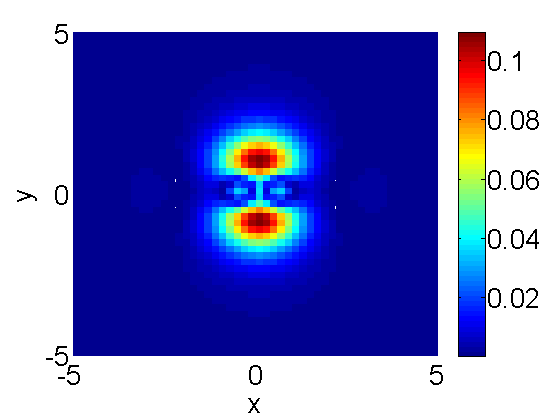
\includegraphics[width=\linewidth]{BestFitVsSimpleIter/ChristovIC_50_bt5_c017_h02_O(h^6).png}
		\centerline{$c=0.17$}
		\centerline{$\beta = 1,3,5$ (от горе надолу) }
	\end{minipage}
	\begin{minipage}[b]{0.48\linewidth}
		\raggedright
		 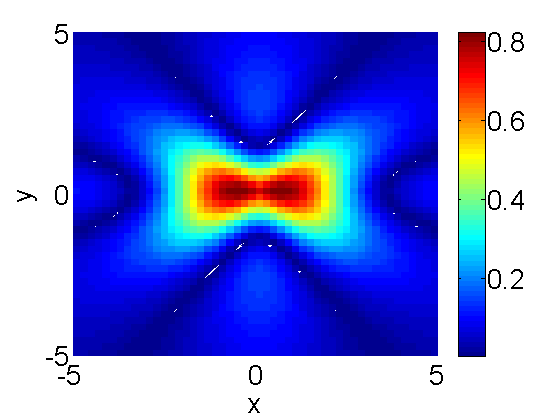
\includegraphics[width=\linewidth]{BestFitVsSimpleIter/ChristovIC_50_bt1_c090_h02_O(h^6).png}
		\centerline{$\beta = 1$}
		\centerline{$c = 0.1, 0.5, 0.9$ (от горе надолу)}
	\end{minipage}
	\caption{Разликите между числено решение $v$ получено с ``Метода на простата итерация'' и ``best-fit'' формулите $v^*$ от \cite{Ch2011}. }
	\label{fig:difference}
\end{figure}

\subsection{Сравнение с ``best--fit'' формулите от \cite{Ch2011} }
Фигура \ref{fig:difference} заедно с Таблици \ref{tab:diff-beta1}, \ref{tab:diff-c017} показват разликите в абсолютна стойност между числено решение получено на последната итерация $v$ и ``best-fit'' формулите $v^*$. Големината на областта при тези тестове е $L_x = L_y = 50$. При дискретизацията са използвани крайни разлики с шести ред на апроксимация $p=6$, стъпката по пространството е $h=0.2$, а граничното условие е описано в ``Симетрично гранично условие по абцисата и ордината при елиптичната задача''. При Таблица \ref{tab:diff-c017}, скоростта $c = 0.17$ е фиксирана, а $\beta=1, 2, 3, 4, 5$ нараства. При Таблица \ref{tab:diff-beta1}, дисперсионния параметър $\beta=1$ е фиксиран, а скоростта $c = 0.1, 0.3, 0.5, 0.7, 0.9$ нараства. Аналогично е разпределението при графиките от Фигура \ref{fig:difference}, които показват абсолютната разлика между двете функции само в подобласт на $\Omega_h$ - $[-5,  5] \times [-5,5]$, където е най-голема. Параметърът $\alpha = 1$ е фиксиран. За да получим съпоставката между двете функции коректно в $\Omega_h$ и имайки предвид смяната на променливите направена в уравнение \rf{eq3} се получава:
\be
v^*\left(\sqrt{\beta}x_i,\sqrt{\beta}y_j\right)-v(x_i,y_j), \quad (x_i,y_j) \in \Omega_h
\ee
Нека $D^*_{\kappa}$ да дефинира процентната разликата между двете решения $v$ и $v^*$ в ${L_2 }$ и ${L_\infty}$ норми, върху цялата област $\Omega_h$:
\be\label{diffvv}
D^*_{\kappa} := 100 \times \frac{\Vert v^*-v \Vert_{\kappa} }{ \Vert v \Vert_{\kappa} }.
\ee
Целта е $D^*_{\kappa}$ да служи като обективен показател, който измерва големината на отклонението $v^*(\sqrt{\beta}x,\sqrt{\beta}y)-v(x,y)$, където с $\kappa$ е означена използваната норма - ${L_2 }$ или ${L_\infty}$.
%================================================================

\begin{table}[ht]
\centering
\begin{tabular}{|l|c|l l|l l|}
\hline 
\hline 
$\beta$	& c 	& $\|v^*-v \|_{L_2 }$ & $\|v^*-v \|_{L_\infty }$  	& $D^*_{L_2}$	& $D^*_{L_\infty }$	\\
\hline 
1& 		0.1	&	1.4772e-01 		& 	8.1024e-03 				& 2.7\%			& 1.7\%		\\
\hline 
1& 		0.3 	&	1.4310e-01 		& 	8.7770e-03				& 2.7\%			& 1.9\%		\\
\hline 
1& 		0.5 	&	1.6934e-01 		& 	1.3332e-02				& 3.5\%			& 3.3\%		\\
\hline 
1& 		0.7 	&	5.8673e-01		& 	5.1122e-02				& 14.8\%		& 16.2\%	\\
\hline 
1& 		0.9	&	2.1599e+0 		& 	1.6439e-01				& 93.1\%		& 121.2\%	\\
\hline 
\hline 
\end{tabular}
\caption{Разликите между числено решение $v$ получено с ``Метода на простата итерация'' и ``best-fit'' формулите $v^*$ от \cite{Ch2011} при $\beta=1$ и $c=0.1, 0.3, 0.5, 0.7, 0.9$.}
\label{tab:diff-beta1}
\end{table}
От Таблица \rf{tab:diff-beta1} се вижда, че разликата между двете дискретни функции в $L_2$ норма се увеличава от $2.7\%$ до $93.1\%$, а при $L_\infty$ норма - от $1.7\%$ до $121.2\%$, когато параметърът $c$ расте. Формулата $v^*$ представлява числено решение, което използва развитие в ред около скоростта $c$. Затова при по-големи скорости процентът $D^*_{\kappa}$ нараства рязко, както е описано в \cite{Ch2011}.

%================================================================

\begin{table}[ht]
\centering
\begin{tabular}{|l|c|l l| c|l|c|l l|}
\hline 
\hline 
$\beta$	& c 	& $\|v^*-v \|_{L_2 }$ & $\|v^*-v \|_{L_\infty }$  	& $D^*_{L_2}$	& $D^*_{L_\infty }$	\\
\hline 
1& 		0.17&	1.4704e-01 		& 	8.3793e-03 				& 2.7\%			& 1.8\%		\\
\hline 
2& 		0.17&	1.2688e-01 		& 	9.0013e-03				& 3.3\%			& 1.9\%		\\
\hline 
3& 		0.17&	1.3803e-01 		& 	1.3134e-02				& 4.4\%			& 2.8\%		\\
\hline 
4& 		0.17&	 1.5240e-01 		& 	1.7228e-02				& 5.7\%			& 3.7\%		\\
\hline 
5& 		0.17&	1.6720e-01 		& 	2.1844e-02				& 7.0\%			& 4.6\%		\\
\hline 
\hline 
\end{tabular}
\caption{Разликите между числено решение $v$ получено с ``Метода на простата итерация'' и ``best-fit'' формулите $v^*$ от \cite{Ch2011} при $\beta=1, 2, 3, 4, 5$ и $c=0.17$.}
\label{tab:diff-c017}
\end{table}
%================================================================
При Таблица \rf{tab:diff-c017} се получават сходни резултати. При по-големи стойности за $\beta$, процентната разлика нараства до $7.0\%$ и $4.6\%$ съответно в $L_2$ и $L_\infty$ норми. Описаните разлики при повечето от разгледани случаи се оказват достатъчно големи и водят до разпадане на вълната дори и при малка скорост от $c=0.27$ и $\beta = 3$, както е показано в \cite{ref21, dani, milenaDani}. Този пример е разгледан по-надолу в настоящата работа в частта ``Числен тест за хиперболичната задача при параметри $\beta = 3$ и $c=0.27$'', където е показано, че формата и максимума на вълната се запазват за времевия интервал $[0, 10]$, ако за начално условие се изполва решението от ``Метода на простата итерация'' приложен за елиптичната задача. 

\section{Ново гранично условие за двумерното елиптично уравнение \rf{eq3}}
Трябва да се отбележи, че както елиптичното така и хиперболичното уравнения са дефинирани в цялата равнина $\RR^2$. За да се решат тези уравнения числено се въвежда краен правоъгълник, върху който се построява мрежа $\Omega_h$. Така могат да се получат резултати, които апроксимират непрекъснатото решение в неограничената област, като целият процес трябва да приключи за разумно време (не повече от два-три дни при най-ситните стъпки $h$ и $\tau$). В случай, че за уравнение \rf{eq3} се приложи гранично условие по краищата на областта $\partial \Omega_h$, то със сигурност изчислителната сложност ще намалее използвайки по-малки области особено при Тест 2 ($\Omega_h = [-128, 128] \times [-58, 58]$). Гранично Условие (ГУ), което се използва тук, е познато в литературата като абсорбиращо ГУ (виж \cite{ref31} при вълнови уравнения, \cite{ref32} при уравнения от типа на Хелмхолц, \cite{ref33} за елиптични уравнения от втори ред и т.н.). Задачата за намиране на гранично условие е разгледана в \cite{ref116}, където е открита следната асимптотика за търсената функция $v$:
\be
v(x,y) = v(r) ~ \frac{C_u}{r^2}, \quad r>>1
\ee
за достатъчно големи стойности $r = \sqrt{x^2 + y^2}$. Тази част на дисертацията изследва едно ново гранично условие за стационарното ПУБ \rf{eq3}:
\be\label{bndK}
\tilde v(x,y) = \mu_v \frac{ (1-c^2)x^2 - y^2}{ ((1-c^2)x^2 - y^2)^2}, \quad x^2 + y^2 >> 1.
\ee
Получаването на последната формула е процес, при който първоначално са разгледани отделните членове в уравнение \rf{eq3} и тяхната асимптотика далеч от максимума на решението в нулата. Впоследствие, на базата на извършения числен анализ е направено допускане за водещите членове в уравнението, които са отговорни за асимптотиката на решението на безкрайност. Така елиптичното уравнение \rf{eq3} се опростява до уравнение на Лаплас с помощта на няколко смени на променливите. За уравнението на Лаплас е изведено аналитичното решение \rf{bndK}, което зависи единствено от координатите $(x,y)$, скоростта $c$ и произволен параметър $\mu_v$. В заключение, посредством серия от числени експерименти, е показана валидността на гранична функция \rf{bndK}. 

Уравнение \rf{eq3} е еквивалентно на 
\begin{align}\label{eq3full}
&\beta v_{xx} + \beta (1-c^2) v_{yy} - v_{xxxx} - (2-\beta c^2)v_{xxyy} - (1-\beta c^2)v_{yyyy} \nonumber \\ 
&- \alpha \beta (v^2)_{xx} - \alpha \beta (v^2)_{yy}  =0.
\end{align}
Взимайки предвид факта, че функцията $v(r)$ има асимптотика $O(r^{-2})$, то очакването е, че за големи стойности на $r >> 1$ членовете $\beta v_{xx}$ и $\beta (1-c^2) v_{yy}$ ще имат асимптотика $O(r^{-4})$, а останалите събираеми в уравнението \rf{eq3full}:
\be
- v_{xxxx},  - (2-\beta c^2)v_{xxyy},  - (1-\beta c^2)v_{yyyy}, - \alpha \beta (v^2)_{xx}, - \alpha \beta (v^2)_{yy}
\ee
ще имат асимптотика, която е $O(r^{-6})$. Така за големи стойности на $r$, пренебрегвайки частите с по-нисък порядък $O(r^{-6})$, остават два водещи члена:
\be\label{asymptEq}
\beta \tilde v_{xx} + \beta (1-c^2) \tilde v_{yy} =0, \quad \tilde v(x,y) ~ \frac{1}{x^2 + y^2}, \quad x^2 + y^2 >>1.
\ee
Вида на отделните членове е описан в серия от експериметни и може да се види на Фигури \ref{fig:assympt_c017bt1}, \ref{fig:assympt_c017bt3} и \ref{fig:assympt_c017bt5}, където $c=0.17$ е фиксирано, а $\beta = 1, 3, 5$ се мени и Фигури \ref{fig:assympt_beta1c01}, \ref{fig:assympt_beta1c05} и \ref{fig:assympt_beta1c09}, където $\beta=1$ е фиксирано, а $c = 0.1, 0.5, 0.9$ се мени. Съответните числени тестове показани на картинките са направени при големина на областта $\Omega_h = [-50, 50] \times [-50, 50]$, с метод на Тейлор, шести ред апроксимация $p=6$, стъпка по пространството $h=0.2$, $\alpha = 1$ и праг на спиране $\epsilon \le 5 \times 10^{-10}$. Използвано е гранично условие описано в частта ``Симетрично гранично условие по абцисата и ординатата при елиптичната задача'' заедно с ``метода на простата итерация''. Представените графики са в логаритмични скали по $x,y$. На всяка страница долната легенда е обща и за двете картинки с цел по-добро представяне на резултатите. Константите $\gamma_1$, $\gamma_2$ и $\gamma_3$ са коефициентите пред съответните членове от уравнението както следва
\begin{align*}
\gamma_1 = \beta (1-c^2) \\
\gamma_2 = (1-\beta c^2) \\
\gamma_3 = (2-\beta c^2).
\end{align*}
Останалите константи $\gamma_4$, $\gamma_5$, $\gamma_6$ и $\gamma_6$ са подходящо избрани за всяка двойка графики, така че функциите $(r^{-4}, |v_{xx}|)$ и $(r^{-6}, |- (2-\beta c^2)v_{xxyy}|)$ да са равни в началото (при $r=x=20$ на горния панел и при $r=y=20$ на долния панел).
Основния извод е, че водещите членове с най-голяма абсолютна стойност са $\beta v_{xx}$ и $\beta (1-c^2) v_{yy}$, а останалите са по-малки. Остатъкът $R$ от \rf{residual}, който също е представен на графиката, е сума от всички членове в уравнението \rf{eq3full} и той е най-малък по абсолютна стойност, т.е. уравнението е удовлетворено числено в разгледаните интервали. 
Изобразявайки функцията $\Psi : \RR \rightarrow \RR$, с уточнението че $\Psi(r) = r^{-n}, n \in \mathbb{N}$, в логаритмични скали представлява граф от вида $(\rho, -n \rho )$, където $\rho := log_{10}(r)$ и $ -n \rho = log_{10}( \Psi(r) ) $, т.е. това е линейна функция с наклон $-n$. Същото свойство е видно и на всички графики от Фигурите \ref{fig:assympt_c017bt1} - \ref{fig:assympt_beta1c09}. Посредством помощните функции $\gamma_4 y^{-4}$, $\gamma_5 y^{-6}$, $\gamma_6 x^{-4}$ и $\gamma_7 x^{-6}$ се открояват различните наклони при членовете $\beta v_{xx}$ и $\beta (1-c^2) v_{yy}$ с асимптотика $O(r^{-4})$ и 
$$
- v_{xxxx},  - (2-\beta c^2)v_{xxyy},  - (1-\beta c^2)v_{yyyy}, - \alpha \beta (v^2)_{xx}, - \alpha \beta (v^2)_{yy}
$$
с асимптотика $O(r^{-6})$, които са съответно $-4$ и $-6$.
\begin{figure}[ht]
	\begin{minipage}[b]{0.95\linewidth}
		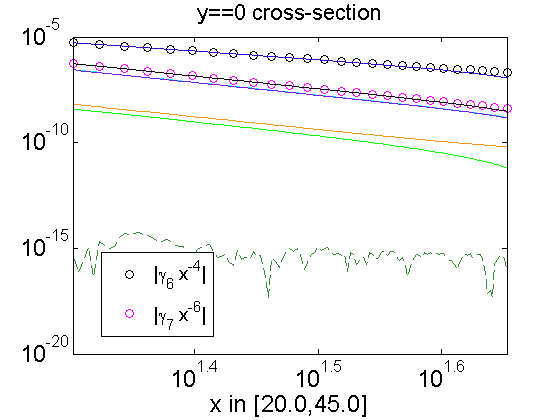
\includegraphics[width=\linewidth]{AssymptForEachTerm/c017_bt1_5/ChristovIC_AlongX_50_ZB2_bt1_c017_h020_O(h^6).png}
	\end{minipage}
	\begin{minipage}[b]{0.95\linewidth}
		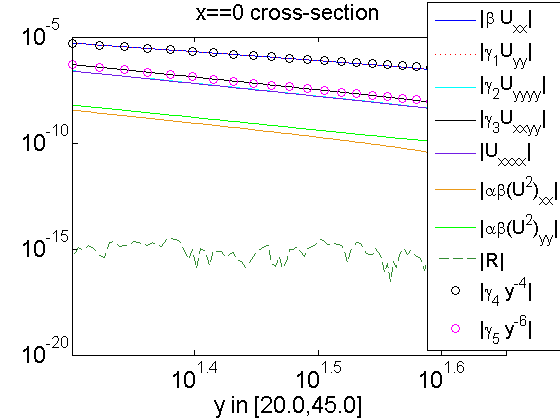
\includegraphics[width=\linewidth]{AssymptForEachTerm/c017_bt1_5/ChristovIC_AlongY_50_ZB2_bt1_c017_h020_O(h^6).png}
	\end{minipage}
	\caption{Асимптотичното поведение на членовете от уравнение \rf{eq3full}, представени в абсолютна стойност и логаритмични скали по $x,y$, получено с ``Метода на простата итерация'' и нулево гранично условие. Скоростта и дисперсионния параметър са $\boldsymbol{c=0.17}$ и $\boldsymbol{\beta = 1}$. }
	\label{fig:assympt_c017bt1}
\end{figure}
\FloatBarrier
\begin{figure}[ht]
	\begin{minipage}[b]{0.95\linewidth}
		\raggedleft
		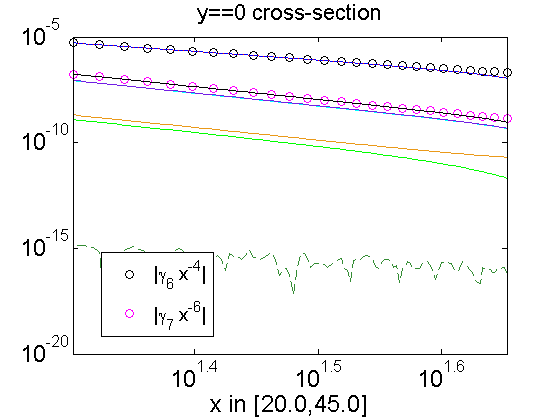
\includegraphics[width=\linewidth]{AssymptForEachTerm/c017_bt1_5/ChristovIC_AlongX_50_ZB2_bt3_c017_h020_O(h^6).png}
	\end{minipage}
	\begin{minipage}[b]{0.95\linewidth}
		 \raggedright
		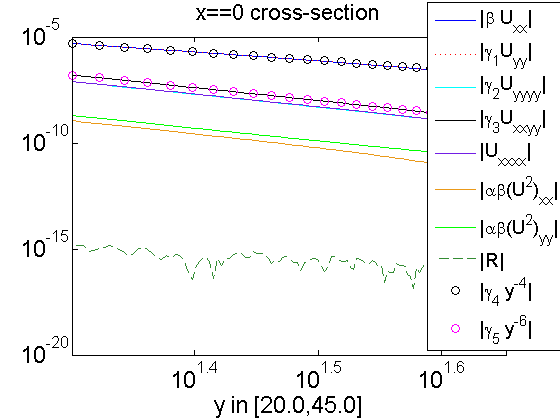
\includegraphics[width=\linewidth]{AssymptForEachTerm/c017_bt1_5/ChristovIC_AlongY_50_ZB2_bt3_c017_h020_O(h^6).png}
	\end{minipage}
	\caption{Асимптотичното поведение на членовете от уравнение \rf{eq3full}, представени в абсолютна стойност и логаритмични скали по $x,y$, получено с ``Метода на простата итерация'' и нулево гранично условие. Скоростта и дисперсионния параметър са $\boldsymbol{c=0.17}$ и $\boldsymbol{\beta = 3}$.}
	\label{fig:assympt_c017bt3}
\end{figure}
\FloatBarrier
\begin{figure}[ht]
	\begin{minipage}[b]{0.95\linewidth}
		\raggedleft
		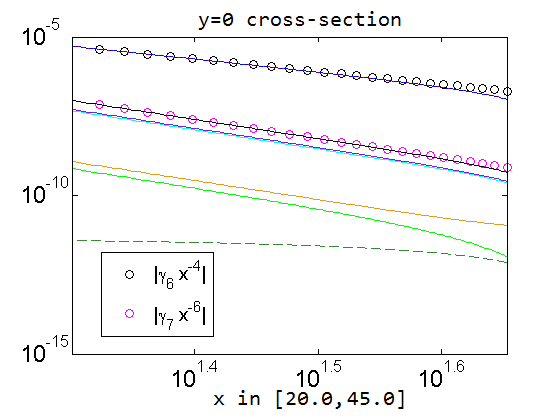
\includegraphics[width=\linewidth]{AssymptForEachTerm/c017_bt1_5/ChristovIC_AlongX_50_ZB2_bt5_c017_h020_O(h^6).png}
	\end{minipage}
	\begin{minipage}[b]{0.95\linewidth}
		 \raggedright
		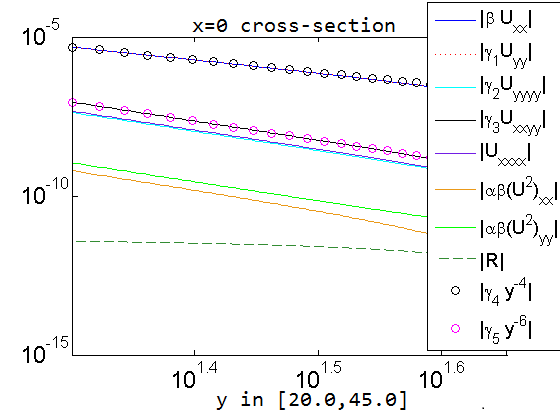
\includegraphics[width=\linewidth]{AssymptForEachTerm/c017_bt1_5/ChristovIC_AlongY_50_ZB2_bt5_c017_h020_O(h^6).png}
	\end{minipage}
	\caption{Асимптотичното поведение на членовете от уравнение \rf{eq3full}, представени в абсолютна стойност и логаритмични скали по $x,y$, получено с ``Метода на простата итерация'' и нулево гранично условие. Скоростта и дисперсионния параметър са $\boldsymbol{c=0.17}$ и $\boldsymbol{\beta = 5}$.}
	\label{fig:assympt_c017bt5}
\end{figure}
\FloatBarrier
%end----------------
\begin{figure}[ht]
	\begin{minipage}[b]{0.95\linewidth}
		\raggedleft
		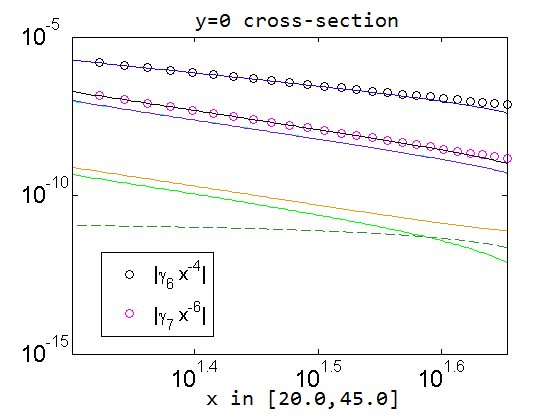
\includegraphics[width=\linewidth]{AssymptForEachTerm/bt1_c010_090/ChristovIC_AlongX_50_ZB2_bt1_c010_h020_O(h^6).png}
	\end{minipage}
	\begin{minipage}[b]{0.95\linewidth}
		 \raggedright
		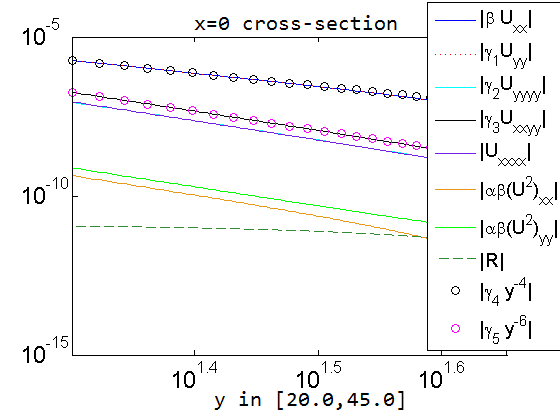
\includegraphics[width=\linewidth]{AssymptForEachTerm/bt1_c010_090/ChristovIC_AlongY_50_ZB2_bt1_c010_h020_O(h^6).png}
	\end{minipage}
	\caption{Асимптотичното поведение на членовете от уравнение \rf{eq3full}, представени в абсолютна стойност и логаритмични скали по $x,y$, получено с ``Метода на простата итерация'' и нулево гранично условие. Скоростта и дисперсионния параметър са $\boldsymbol{c=0.1}$ и $\boldsymbol{\beta = 1}$. }
	\label{fig:assympt_beta1c01}
\end{figure}
\FloatBarrier

\begin{figure}[ht]
	\begin{minipage}[b]{0.95\linewidth}
		\raggedleft
		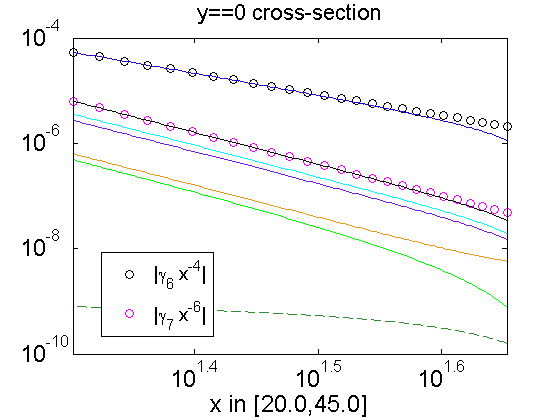
\includegraphics[width=\linewidth]{AssymptForEachTerm/bt1_c010_090/ChristovIC_AlongX_50_ZB2_bt1_c050_h020_O(h^6).png}
	\end{minipage}
	\begin{minipage}[b]{0.95\linewidth}
		 \raggedright
		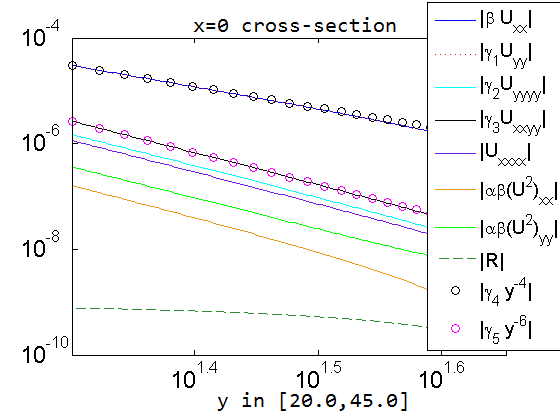
\includegraphics[width=\linewidth]{AssymptForEachTerm/bt1_c010_090/ChristovIC_AlongY_50_ZB2_bt1_c050_h020_O(h^6).png}
	\end{minipage}
	\caption{Асимптотичното поведение на членовете от уравнение \rf{eq3full}, представени в абсолютна стойност и логаритмични скали по $x,y$, получено с ``Метода на простата итерация'' и нулево гранично условие. Скоростта и дисперсионния параметър са $\boldsymbol{c=0.5}$ и $\boldsymbol{\beta = 1}$. }
	\label{fig:assympt_beta1c05}
\end{figure}
\FloatBarrier

\begin{figure}[ht]	
	\begin{minipage}[b]{0.95\linewidth}
		\raggedleft
		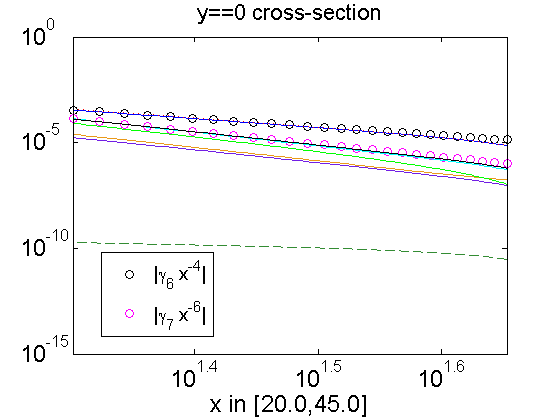
\includegraphics[width=\linewidth]{AssymptForEachTerm/bt1_c010_090/ChristovIC_AlongX_50_ZB2_bt1_c090_h020_O(h^6).png}
	\end{minipage}
	\begin{minipage}[b]{0.95\linewidth}
		 \raggedright
		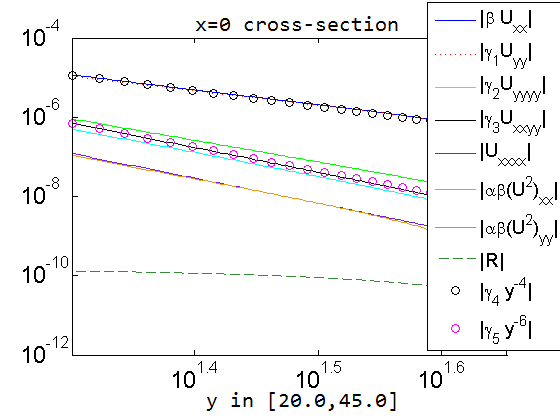
\includegraphics[width=\linewidth]{AssymptForEachTerm/bt1_c010_090/ChristovIC_AlongY_50_ZB2_bt1_c090_h020_O(h^6).png}
	\end{minipage}
	\caption{Асимптотичното поведение на членовете от уравнение \rf{eq3full}, представени в абсолютна стойност и логаритмични скали по $x,y$, получено с ``Метода на простата итерация'' и нулево гранично условие. Скоростта и дисперсионния параметър са $\boldsymbol{c=0.9}$ и $\boldsymbol{\beta = 1}$. }
	\label{fig:assympt_beta1c09}
\end{figure}
\FloatBarrier
Следната смяна $\bar x  = \sqrt{1-c^2} x$, $\bar y = y$ и $\tilde V (\bar x, \bar y)$ на променливите трансформира \rf{asymptEq} в уравнението на Лаплас:
\be\label{LaplaceEq}
\Delta \tilde V(\bar x, \bar y) = 0, \quad \tilde V(\bar x, \bar y) = \frac{1}{\bar r^2}, \quad \bar r = \sqrt{\bar x^2 + \bar y^2} \rightarrow \infty.
\ee
Последното в полярни координати има следния вид:
\begin{align}\label{LaplacePolar}
&\frac{\partial^2}{\partial \bar r^2} \tilde V_p(\bar r,\bar \phi) + \frac{1}{\bar r} \frac{\partial}{\partial \bar r} \tilde V_p(\bar r, \bar \phi) + \frac{1}{\bar r^2} \frac{\partial^2}{\partial \bar \phi^2} \tilde V_p(\bar r, \bar \phi) = 0 \\
&\bar \phi = arctan(\frac{\bar y}{\bar x}) \nonumber
\end{align}
След разделяне на променливите $\tilde V_p(\bar r, \bar \phi) = H(\bar r) G(\bar \phi)$ в \rf{LaplacePolar} за решението му се получават следните функции:
\begin{align}\label{LaplaceSol}
&H(\bar{r}) = \sum^{\infty}_{n=0} (\mu_{1,n} \frac{1}{ \bar{r}^n} + \mu_{2,n} \bar{r}^n ),
\\ \nonumber &G(\bar \phi) = \sum^{\infty}_{n=0} (\mu_{3,n}sin(n \bar \phi ) + \mu_{4,n}cos(n \bar \phi)),
\end{align}
където $\mu_{1,n}, \mu_{2,n}, \mu_{3,n}, \mu_{4,n}, n \in \mathbb{N}_{0}$ са реални константи. Първата функция се опростява до вида
\be
H(\bar r) = \mu_{1,2}\frac{1}{\bar r^2}, \quad \mu_{1,n} = 0, n \neq 2, \quad \mu_{2,n} = 0, n \ge 0
\ee
знаейки, че решението има асимптотика от вида $1/r^2$. За втората функция се получава
\be
G(\bar \phi) = \mu_{4,2}cos(2 \bar \phi), \quad \mu_{3,n} = 0, n \ge 0, \quad \mu_{4,n} = 0, n \neq 2.
\ee
знаейки, че решението за достатъчно големи $r >> 1$ е положително върху абцисата и отрицателно върху ординатата (по посока на движение на вълната). Крайната формула за решението на \rf{LaplacePolar} е:
\be \label{LaplaceSol2}
\tilde V_p(\bar r, \bar \phi) = \mu_v \frac{ cos(2 \bar \phi) }{ \bar r^2 } = \mu_v \frac{ cos(\bar \phi)^2 - sin(\bar \phi)^2 }{ \bar r^2 } = \mu_v \frac{ \bar x^2 - \bar y^2 }{ (\bar x^2 + \bar y^2)^2 },
\ee
където $\mu_v = \mu_{1,2} \mu_{4,2}$. В старите $(x, y, r=\sqrt{x^2+y^2})$ координати \rf{LaplaceSol2} е еквивалентно на 
\be\label{bndv}
\tilde v(x, y) = \mu_v \frac{ (1-c^2) x^2 - y^2 }{ ((1-c^2) x^2 + y^2)^2 }.
\ee
Параметърът $\mu_v$ се намира чрез минимизиране на 
\begin{equation}\label{eqMin}
\mu_v = \min_{ \mu_v > 0 } || \tilde v( x_i, y_j) - \widehat v^{(k)}_{i,j} ||_{L_2}, \quad (x_i, y_j) \in \omega_B ,
\end{equation}
където 
\be\label{omegaB}
\omega_B = \{ (x_i, y_j) \in \omega_h \: | \: x_i > \frac{3L_x}{4}, y_j > \frac{3L_y}{4} \},
\ee
а с $\widehat v^{(k)}$ е означено решението получено при $k$-тата итерация от процедурата \rf{eq55}. Минимизационната задача дефинирана в \rf{eqMin} е еквивалента на решаването на линейно уравнение спрямо $\mu_v$. Централните крайни разлики използвани при апроксимацията на оператора на Лаплас и описани в Таблица \rf{table:A00} не се променят по границата $x=L_x$ и $y=L_y$. За целта при $p=2$ областта $\omega_h$ се разширява по $x$ и по $y$ с една стъпка $h$, при $p=4$ с две стъпки $2h$ и при $p=6$ с три стъпки $3h$.
Стойностите на $\widehat v$ във възлите от увеличената област, които са извън $\omega_h$, се изчисляват използвайки граничната функция $\tilde v(x, y)$.

\section{Числени резултати от ``метода на простата итерация'' получени с новото ГУ}
Два числени теста са направени за валидация на формула \rf{bndv}. Първия експеримент разглежда поведението на константата $\mu_v$ и резултата от минимизационната процедура \rf{eqMin} при нарастване на областта. Втория тест разглежда поведението на функцията $\widehat v$ и нейната асимптотика по $x,y$ осите.
\subsection{Експеримент 1 за ГУ \rf{bndv}}
В тази част са използвани диференчни схеми с четвърти ред на апроксимация $p=4$ и параметрите в \rf{eq55} са дефинирани както следва: $\alpha = 1$, $\beta = 3$ и $c=0.45$. Разгледани са четири различни по големина области $\omega_h = [0, L_x] \times [0, L_y]$, където $L_x = L_y = 20, 40, 80, 160$ и фиксирана стъпка по пространството $h=0.5$. На Таблица \rf{tab:valBnd1} са представени резултати получени в края на итеративната процедура \rf{eq55} и прилагайки ГУ от \rf{bndv}. Първата колона описва размера на областта. Във втората колона е показана стойността на функцията $\widehat{v}_{i,j}$ в точката: ${x}_i = 0$, $ {y}_j =   L_{ y}$. Поведението на параметъра $\mu_v$ е представено в третата колона. Най-накрая се вижда разликата между граничната функция \rf{bndv} и численото решение $\widehat{v}$ от последната итерация върху $\omega_B$ в $L_2$ норма.
\begin{table}[ht]
\centering
		\begin{tabular}{||c||c|c|c||}
			\hline
			\hline
      $ L_{ x} = L_{ y}$        &         $\widehat{v}_{i,j}^k$ в  $({x}_i, {y}_j) = (0, L_{ y})$    &    $\mu_v$  &   \mbox{$min|| \tilde v( x_i, y_j) - \widehat v ^k_{i,j} ||_{L_2,\omega_B}$}\\
   			\hline
			\hline
      20    & -2.23e-04    &  1.9355e-01  &     4.17e-05  \\
               	 \hline
    40      & -5.65e-05   &   1.9369e-01    &    4.42e-06 \\
			\hline 	
      80    & -1.41e-05  &      1.9378e-01      &       7.56e-07  \\
			\hline 	
     160     & -3.53e-06  &    1.9381e-01        &     7.44e-10 \\
		   \hline
	             \hline
                     \end{tabular}
\caption{Свойства на решението и ГУ при различни големини на областта $\omega_h$.}
\label{tab:valBnd1}
\end{table}
\FloatBarrier
Резултатите от Таблица \rf{tab:valBnd1} показват, че стойностите $\mu_v$ се установяват, понеже разликата между две последователни стойности намалява с увеличаването на областта. В допълнение, стойността на функцията $\widehat v(0,L_y)$ намалява с темп от вида $1/r^2$. Разликите между численото решение $\widehat v$ и граничната функция $\tilde v$ в $\omega_B$ намаляват при по-големи размери $L_x, L_y$. 
\subsection{Експеримент 2 за ГУ \rf{bndv}}
В тази част са разгледани различни аспекти от асимптотиката на численото решение. Тук размерът на областта $\omega_h = [0, 50] \times [0, 50]$ е фиксиран. Използвани са диференчни схеми с четвърти ред на апроксимация $p=4$ и параметрите в \rf{eq55} са дефинирани както следва: $\alpha = 1$, $\beta = 3$ и $c=0.45$. Единствено стъпката по пространството се мени $h=0.1, 0.2, 0.4, 0.8$.
\begin{figure}[ht]
	\begin{minipage}[b]{0.5\linewidth}
		\raggedleft
		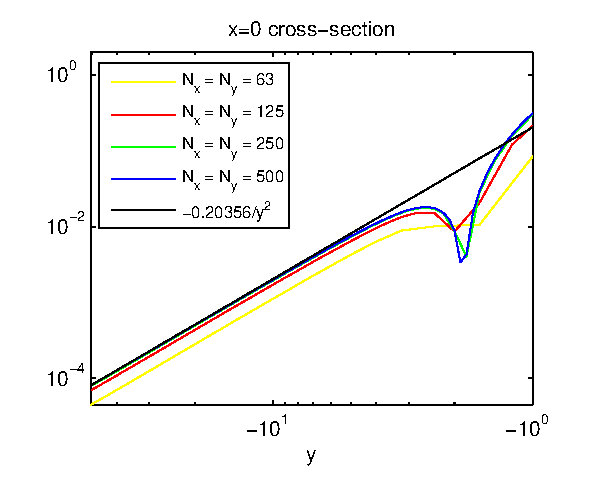
\includegraphics[width=\linewidth]{NewBoundaryCondition/crossSectionLogX=0.eps}
	\end{minipage}	
	\begin{minipage}[b]{0.5\linewidth}
		\raggedright
		 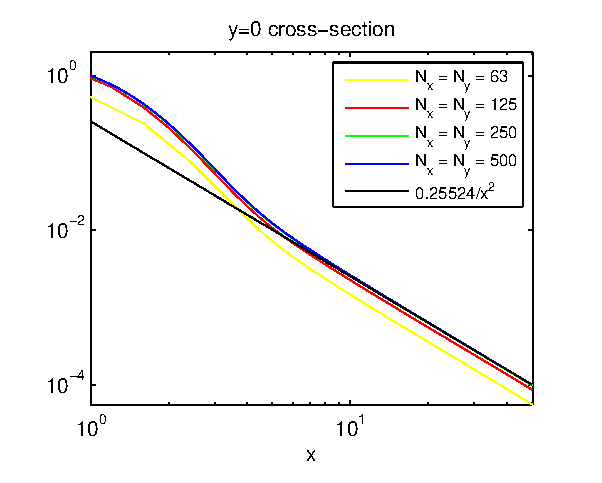
\includegraphics[width=\linewidth]{NewBoundaryCondition/crossSectionLogY=0.eps}
	\end{minipage}
	\begin{minipage}[b]{0.5\linewidth}
		\raggedleft
		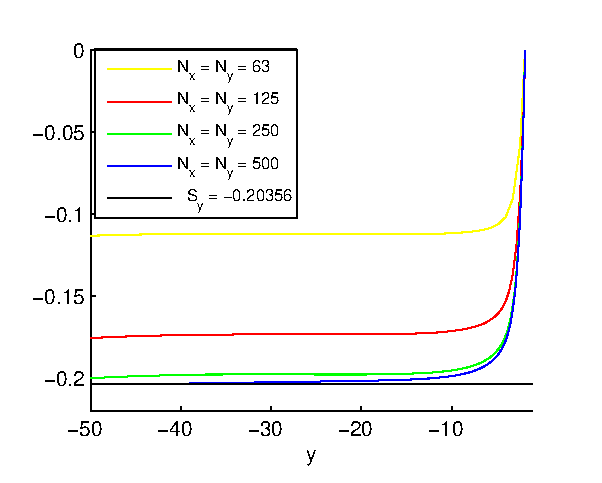
\includegraphics[width=\linewidth]{NewBoundaryCondition/crossSectionX=0FF.eps}
	\end{minipage}	
	\begin{minipage}[b]{0.5\linewidth}
		\raggedright
		 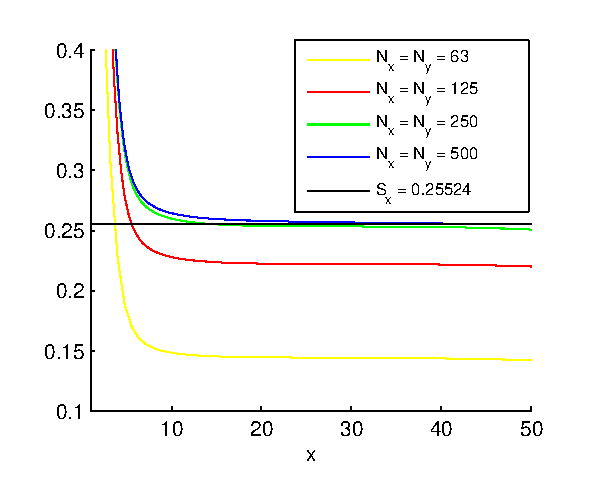
\includegraphics[width=\linewidth]{NewBoundaryCondition/crossSectionY=0FF.eps}
	\end{minipage}
	\caption{Ефектът от промяната на дискретната стъпка по пространството $h=0.1, 0.2, 0.4, 0.8$. На горните панели се вижда функцията $\widehat{v}$ в логаритмични скали по $x,\widehat v(x,0)$ и $y,\widehat v(0,y)$. На долните панели са разположени следните криви: $(y, y^2 \widehat v(0,y)), \; (x, x^2 \widehat v(x,0))$. }
	\label{fig:bndCross}
\end{figure}
\FloatBarrier
Горните две графики от Фигура \ref{fig:bndCross} представят решението в абсолютна стойност върху логаритмични скали по осите $(y,\widehat v(0,y) )$ и $(x,\widehat v(x,0))$. Ясно се вижда, че численото решение за всяка от стъпките $h$ следва наклона на функцията $1/r^2$ за достатъчно големи $r >> 1$. Долните две графики показват численото решение скалирано с множител $r^2$, т.е. това са кривите $(y, y^2 \widehat v(0, y) )$ и $(x, x^2 \widehat v(y, x) )$. Скалирания профил на решението апроксимира константа: $s_y=-0.20356$ (за левия панел) и $s_x=0.25542$ (за десния панел), за достатъчно големи $r >> 1$. Тези графики са в съответствие с новото ГУ от \rf{bndv} и асимптотиката намерена в \cite{ref116}. В допълнение, използвайки \rf{bndv} за гореописаните случаи при $x=0$ и $y=0$, може да се изведат следните изрази:
\be
\tilde v(0, y) = -\mu_u \frac{1}{y^2}, \quad \tilde v(x, 0) = \frac{\mu_u}{(1-c^2)} \frac{1}{x^2}.
\ee
От последните формули се получават константите $s_x$ и $s_y$ показани в долните панели на Фигура \ref{fig:bndCross}.

\subsection{Положителните и отрицателните области на численото решение за Тест 1 и Тест 2}
\begin{figure}[ht]
	\begin{minipage}[b]{0.5\linewidth}
		\raggedleft
		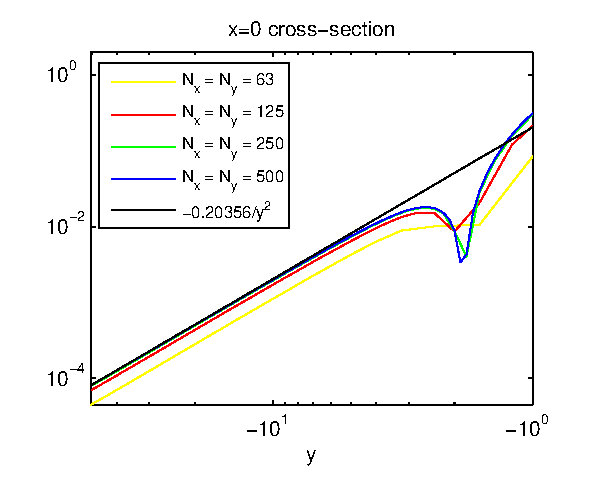
\includegraphics[width=\linewidth]{NewBoundaryCondition/crossSectionLogX=0.eps}
	\end{minipage}	
	\begin{minipage}[b]{0.5\linewidth}
		\raggedright
		 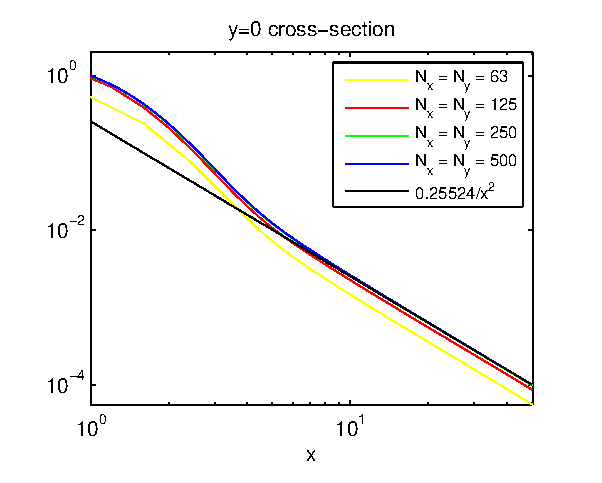
\includegraphics[width=\linewidth]{NewBoundaryCondition/crossSectionLogY=0.eps}
	\end{minipage}
	\caption{Положителните и отрицателните области на численото решение $\widehat v$. }
	\label{fig:posNegDom}
\end{figure}
\FloatBarrier
Фигура \ref{fig:posNegDom} показва знака на численото решение $\widehat v$ получено с граничното условие \rf{bndv} за Тест 1 (левия панел) и Тест 2 (десния панел). Използван е метод на Тейлор с шести ред на апроксимация $p=6$ и $h=0.1$ при Тест 1 и $h=0.2$ при Тест 2. Цветовия интервал е дефиниран както следва: $[-10^{-5}, 10^{-5}]$. Всяка точка под долната граница на интервала $-10^{-5}$ е оцветена в тъмно синьо, а над горната $10^{-5}$ съответно с тъмно червено. Ясно се забелязват очертанията на три области: южна и северна, които са отрицателни и централна, която е положителна. За достатъчно големи стойности $r >> 1$ се забелязва следната зависимост
\begin{align}\label{posNegFromula}
\widehat v(r, \phi) > 0 \quad \text{if} \quad \phi \in (-arctan(\frac{1}{1-c^2}), arctan(\frac{1}{1-c^2}) ) \nonumber\\
\widehat v(r, \phi) < 0 \quad \text{if} \quad \phi \in (arctan(\frac{1}{1-c^2}), \pi - arctan(\frac{1}{1-c^2}) ) \nonumber\\
 \phi = arctan(\frac{ y}{ x})
\end{align}
\section{7.~Conclusion.}
Fourth and sixth order finite difference schemes are applied for numerical evaluation of the stationary traveling wave solutions to the Boussinesq equation in this paper. The high accuracy of the method applied is demonstrated on several experiments. The numerical solution obtained here performs similarly to the numerical solutions given in \cite{Ch2012,Ch2011} with respect to solution shape and the dependence on the velocity $c$ and relative dispersion $\beta$. 
The best-fit approximation formulae from \cite{Ch2011} fail to satisfy the initial equation in the classical sense in the neighborhood of the origin. 
In the future, we will exploit the obtained stationary traveling wave solutions as initial data to the corresponding Boussinesq equation in order to seek two dimensional solitary wave solutions to \rf{eq1}.

\bigskip

%\fi


\section{Увод}
Парадигматично уравнение на Бузинеск
\be\label{problemCh}
...
\ee


\section{Смяна на променливите}

За удобство правим следната смяна на променливите (виж \cite{ref25}):

\begin{align}
x = \sqrt{\beta_1} \bar{x}, \quad y = \sqrt{\beta_1} \bar{y}, \quad t = \sqrt{\beta_1} \bar{t} \nonumber
\end{align}
която променя основното уравнение \rf{problemCh} в
\be\label{problemVC}
 \beta (I-\Delta) \frac{\partial^2}{\partial t^2}u= 
(I-\Delta)\Delta u +\Delta( (\beta - 1 )u - \alpha \beta u^2 )
\ee
където $\beta = \beta_1/\beta_2$. 

\section{Дискретни закони за запазване на енергията и масата при непрекъснатата задача}
В пространството от функции $J_\infty$, които по границата $\partial\Omega$ удовлетворяват $f_b(x) = 0$ и $\Delta f_b(x) = 0$, се дефинира дискретният оператор $A_h$, така че да удовлетворява $A_h v=-\Delta_h v=-v_{\bar{x}x} - v_{\bar{y}y}$. Нека да разгледаме следната диференчната схема
\begin{align}\label{FDS1}
&\beta (E+A_h)v_{\bar{t}t}^{(k)} + A_hv^{(k)}+A_h^2 v^{(k)} -\nonumber\\
&-\frac{\alpha \beta}{3} A_h\left(\frac{(v^{(k+1)})^3-(v^{(k-1)})^3}{(v^{(k+1)}-v^{(k-1)})} \right) + \frac{\beta - 1}{2}A_h\left( v^{(k+1)}+v^{(k-1)} \right) =0
\end{align}
Умножаваме \rf{FDS1} с $A_h^{-1}$ и получаваме
\begin{align}\label{FDS2}
&\beta (E+A_h^{-1})v_{\bar{t}t}^{(k)} + v^{(k)}+A_h v^{(k)} \nonumber\\
&-\frac{\alpha \beta}{3} \frac{(v^{(k+1)})^3-(v^{(k-1)})^3}{(v^{(k+1)}-v^{(k-1)})} + \frac{\beta - 1}{2}\left( v^{(k+1)} + v^{(k-1)} \right)= 0
\end{align}
Ако заместим $v^{(k)}=\frac{1}{2}(v^{(k+1)}+v^{(k-1)})-\frac{\tau^2}{2}v_{\bar{t}t}^{(k)}$ в \rf{FDS2} получаваме
\begin{align*}
&\left( \beta (E+A_h^{-1})- \frac{\tau^2}{2}(E+A_h ) \right)v_{\bar{t}t}^{(k)}  + \frac{1}{2} (E +A_h )(v^{(k+1)}+v^{(k-1)}) \\
&-\alpha \beta \frac{(v^{(k+1)})^3-(v^{(k-1)})^3}{3(v^{(k+1)}-v^{(k-1)})} + \frac{\beta - 1}{2}\left( v^{(k+1)}+v^{(k-1)} \right) = 0.
\end{align*}
Последното уравнение се умножава скаларно с $(v^{(k+1)}-v^{(k-1)})=\tau (v_{\bar{t}}^{(k)} + v_{t}^{(k)})$
\begin{align*}
&\left< \left( \beta (E+A_h^{-1})- \frac{\tau^2}{2}( E+A_h ) \right) \left( \frac{v_{t}^{(k)} - v_{\bar t}^{(k)}}{\tau}   \right ), \tau (v_{\bar{t}}^{(k)} + v_{t}^{(k)}) \right>  + \\
& +\frac{1}{2} \left<  (E +A_h ) \left( v^{(k+1)} + v^{(k-1)} \right ) , v^{(k+1)} - v^{(k-1)} \right> - \\
&- \frac{\alpha \beta}{3} \left< \left( (v^{(k+1)})^3-(v^{(k-1)})^3 \right), 1 \right> + \frac{\beta - 1}{2} \left< \left( (v^{(k+1)})^2-(v^{(k-1)})^2 \right), 1 \right> =0
\end{align*}
след което част от първият член е пренесена във вторият с общ множител $(E + A_h )$ и отчитайки симетричността на оператора $A_h$ ($\left< A_h v,v\right> = \left< v, A_h v\right>$) при втори ред на апроксимация ($p=2$) се получава
\begin{align}\label{EnEnd}
&\left< \bar L  v_{t}^{(k)}, v_{t}^{(k)} \right> - \left< \bar L v_{\bar t}^{(k)}, v_{\bar t}^{(k)} \right>  
 +\frac{1}{4} \left<  (E +A_h ) \left( v^{(k+1)} + v^{(k)} \right ) , v^{(k+1)} + v^{(k)} \right>  -\nonumber \\
&- \frac{1}{4} \left<  (E +A_h ) \left( v^{(k)} + v^{(k-1)} \right ) , v^{(k)} + v^{(k-1)} \right> - \nonumber \\
&- \frac{\alpha \beta}{3} \left< \left( (v^{(k+1)})^3-(v^{(k-1)})^3 \right), 1 \right> + \frac{\beta - 1}{2} \left< \left( (v^{(k+1)})^2-(v^{(k-1)})^2 \right), 1 \right> =0,
\end{align}
където операторът $\bar L$ е дефиниран по следния начин
\begin{align}
\bar L = \beta (E+A_h^{-1})- \frac{\tau^2}{4}( E+A_h ).
\end{align}
Уравнението \rf{EnEnd} важи за всяка точка от пространствената мрежа $(x_i,y_j) \in \Omega_h$. След сумиране на получените уравнения за всички точки от мрежата и допълнителна реорганизация на членовете в уравнението получаваме, че
\be \label{num_en}
E_h(v^{(k)}) =E_h(v^{(k-1)}),
\ee
където
\begin{align}\label{en_norm}
E_h(&V^{(k)})=\left< \left( \beta (E+A_h^{-1})- \frac{\tau^2}{4}( E+A_h ) \right)v_{t}^{(k)} ,v_{t}^{(k)} \right>+ \nonumber\\
&+\frac{1}{4}  \left<  ( E+A_h)(v^{(k+1)}+v^{(k)}), v^{(k+1)}+v^{(k)} \right> - \nonumber\\
&- \frac{\alpha \beta}{3} \left< ((v^{(k+1)})^3,1)+((v^{(k)})^3,1) \right> + \frac{\beta - 1}{2} \left< \left( (v^{(k+1)})^2+(v^{(k)})^2 \right), 1 \right>.
\end{align}
В \rf{EnEnd} сумираме по всички точки от мрежата и затова  $\left< v, q \right>$ се явява скаларното произведение на двата вектора 
\be\label{dotProd}
\left<v, q \right> = \sum_{i=0}^{N_x-1} \sum_{j=0}^{N_y-1} v_{i,j} q_{i,j}.
\ee
Така доказваме следната теорема
\begin{thm}
Решението получено от диференчната схема \rf{FDS1} запазва дискретната енергия $E_h(v^0)$, т.е.  $E_h(v^{(k)}) =E_h(v^{0})$ за всяко $k=1,2,...N_t$.
\end{thm}
По-долу ще наричаме уравнение \rf{FDS1} с името Консервативна схема.
\begin{thm}\label{th1}
Линейната диференчна схема съответстваща на \rf{FDS1} е условно устойчива, когато е изпълнено
$\tau^2 < \frac{4 \beta h^2}{8 + h^2}$ и $\beta \ge 1$.
\end{thm}
Доказателството:
Скаларното произведение \rf{en_norm} без нелинейния член дефинира така наречената Енергиина норма, когато операторите $\bar{L}$ и $(E + A_h)$ са положително дефинирани и ако $\beta \ge 1$. Когато тези условия важат е видно, че \rf{en_norm} може да се ограничи от горе с фиксирано реално число, защото енергията от началното условие ще е същата във всеки един момент от време $\tau k$ според Теорема \rf{th1}. Последното е следствие от изследване на устойчивост при трислойни диференчни схеми в книгата на Самарский \cite{samarski}. Остава да се покаже, че гореспоменатите оператори са положително дефинирани. За целта ще използваме следната Лема:

\begin{lm}\label{lemma1}
Нека $S_n=[s_1,..,s_n]$ е множеството от собствени вектори на реалната матрица $A \in \RR^{n\times n}$,
a $\{\lambda_1,..,\lambda_n\}$ са собствените ѝ стойности, така че $A *s_i = \lambda_i s_i$. Тогава имаме, че $\zeta E + A$, където $\zeta \in \RR$ е реална константа, има същия набор от собствени вектори $S_n$ както $A$, а собствените ѝ стойности са $\{\zeta + \lambda_1,..,\zeta + \lambda_n\}$, така че $(\zeta E + A) * s_i = (\zeta+ \lambda_i) s_i$.
\end{lm}
Доказателство
\be
(\zeta E + A) * s_i = \zeta s_i + A * s_i = \zeta s_i + \lambda_i s_i = (\zeta + \lambda_i) s_i.
\ee
Операторът $-\Delta_{h,2}$ има следните собствени стойности
\begin{align}\label{eigDeltah}
&\lambda_{i,j} = \lambda_{x, i} + \lambda_{y,j} = \frac{4}{h^2}sin^2(\frac{i \pi}{N_x-1}) +  \frac{4}{h^2}sin^2(\frac{j \pi}{N_y-1}) \\
&i = 1,..,N_x-2; \quad j = 1, .. , N_y-2 \nonumber
\end{align}
както е описано в Самарски \cite{samarski}, глава 4.4 ``Свойства на елиптичните диференчни оператори'', с уточнението, че $\lambda_{x, i}$ + $\lambda_{y,j}$ са собствените стойности съответно на $\Delta_{h,2,x}$ и $\Delta_{h,2,y}$. Операторът $-\Delta_{h,2}$ е положително дефиниран, ако всички собствени стойности са положителни $\lambda_{i,j}>0$ и $-\Delta_{h,2}$ е симетричен. Първото следва от \rf{eigDeltah} а второто от структурата на матриците $\Delta_{h,2,x}$ и $\Delta_{h,2,y}$.

Операторът $-\Delta_{h,2}^{-1}$ също е положително дефиниран, защото неговите собствени стойности са $\frac{1}{\lambda_{i,j}} > 0$, а симетрията следва от това, че $-\Delta_{h,2}$ симетричен:
\begin{equation*}
\Delta_{h,2} * \Delta_{h,2}^{-1} = E \Leftrightarrow \Delta_{h,2}^{-T} * \Delta_{h,2}^{T} = E \Leftrightarrow \Delta_{h,2}^{-T} * \Delta_{h,2} = E 
\Leftrightarrow \Delta_{h,2}^{-T} = \Delta_{h,2}^{-1} 
\end{equation*}
Понеже $-\Delta_{h,2}^{-1} > 0$, остава да се покаже, че останалата част в $\bar L$, която е:
\be\label{Lrest}
\frac{4}{\tau^2}\left( \bar L - \beta ( - \Delta_{h,2}^{-1}) \right) = \left( \frac{4 \beta}{\tau^2} - 1\right) E -(-\Delta_{h,2}),
\ee
е положително дефинирана. Очевидно е, че операторът \rf{Lrest} е симетричен, защото $-\Delta_{h,2}$ е симетричен. Използвайки Лема \rf{lemma1} се вижда, че собствените стойности на \rf{Lrest} са
\begin{align}\label{Lrest2}
 &\frac{4 \beta}{\tau^2} - 1 - \frac{4}{h^2}sin^2(\frac{i \pi}{N_x-1}) - \frac{4}{h^2}sin^2(\frac{j \pi}{N_y-1}) > \frac{4 \beta}{\tau^2} - 1 - \frac{8}{h^2}, \\
&i = 1,..,N_x-2; \quad j = 1, .. , N_y-2. \nonumber
\end{align}
Дясната страна в \rf{Lrest2} е положителна при условието, че
\be\label{stabCond}
\frac{4 \beta}{\tau^2} - 1 - \frac{8}{h^2} > 0  \Leftrightarrow \tau^2 < \frac{4 \beta h^2}{8 + h^2}.
\ee

Остана да се покаже, че и операторът $E - \Delta_{h, 2}$ е положително дефиниран без допълнителни условия. Видно е, че той е симетричен, а от Лема \rf{lemma1} за собствените му стойности се получава:
\begin{align}
&1+ \frac{4}{h^2}sin^2(\frac{i \pi}{N_x-1}) + \frac{4}{h^2}sin^2(\frac{j \pi}{N_y-1}) >0, \nonumber\\
&i = 1,..,N_x-2; \quad j = 1, .. , N_y-2 \nonumber
\end{align}
което е положително за всяка двойка $(i, j)$ и следователно $E - \Delta_{h, 2} > 0$. Така се получава, че \rf{en_norm} изпълнява критериите за норма, когато са изпълнени условията \rf{stabCond} и $\beta \ge 1$, с което Теорема \rf{th1} е доказана.

\section{Квадратурни формули за пресмятане на двумерни интеграли}

Масата при непрекъснатата задача \rf{problemVC} се дефинира като
\begin{equation}\label{intM}
D(u(x,y,t))=\int_{\RR^2} u(x,y,t)dx dy
\end{equation}
а енергията 
\begin{align}\label{ex-en}
E(u(x,y,t)):=&\beta \int_{\RR^2} u_t(x,y,t) \: \left(A^{-1}+E\right)u_t(x,y,t) dxdy+
\beta \int_{\RR^2} u^2(x,y,t) dxdy \nonumber\\
+& \int_{\RR^2}u(x,y,t) \left(A u(x,y,t)\right) dxdy
-\frac{2 \alpha \beta}{3} \int_{\RR^2} u^3(x,y,t) dxdy,
\end{align}
където $Au=-\Delta u$ действа във функционалното пространство $J_\infty$ от \rf{funSpace}, а $D(u(x,y,t)) = D(u(x,y,0))$ и $E(u(x,y,t)) = E(u(x,y,0))$ са непрекъснатите маса и енергия за задачата \rf{problemVC} (виж \cite{ref1}). Нека да заменим оператора $Au=-\Delta u$ с неговата дискретна версия $A_hu :=-\Delta_h u$ като използваме апроксимаций от различен ред - $O(|h|^2)$, $O(|h|^4)$, $O(|h|^6)$.
% Ако имаме дискретната производната $u_t$ изчислена с апроксимации също от втори, четвърти и шести ред - $O(\tau^2)$, $O(\tau^4)$, $O(\tau^6)$ - то тогава може да приложим квадратурни формули %за численото пресмятане на енергията \rf{ex-en}.
Следният интеграл дефиниран в област $[a_1, b_1] \times [a_2, b_2]$
\begin{equation}\label{int}
D_h(u(x,y))=\int_{a_1}^{b_1} \int_{a_2}^{b_2} u(x,y)dx dy
\end{equation}
$$x_i, ~i=0,1,...,N_x-1; \;x_0=a_1,~x_{N_x}=b_1, \;h_1=(b_1-a_1)/(N_x-1),$$
$$y_j, ~j=0,1,...,N_y-1; \; y_0=a_2,~y_{N_y}=b_2, \;h_2=(b_2-a_2)/(N_y-1)$$
може да се изчисли посредством двумерни квадратурни формули както е описано по-долу.

\subsection{ 2Д формула на трапците с глобална грешка $O(|h_1|^2+|h_2|^2)$ }

Апроксимацията на интеграла \eqref{intM} с грешка $O(|h_1|^2+|h_2|^2)$ е

\begin{align}\label{quadr2}
D_h(u_{i,j}) =& \sum_{i=1}^{N_x-1} \sum_{j=1}^{N_y-1} h_1 h_2 u_{i,j}
+\frac{h_1}{2}\sum_{i=0} \sum_{j=1}^{N_y-1} h_2 u_{i,j}
+\frac{h_1}{2}\sum_{i=N_x} \sum_{j=1}^{N_y-1} h_2 u_{i,j} \nonumber\\
+&\frac{h_2}{2}\sum_{j=0} \sum_{i=1}^{N_x-1} h_1 u_{i,j}
+\frac{h_2}{2}\sum_{j=N_y} \sum_{i=1}^{N_x-1} h_1 u_{i,j}
\nonumber\\
+&\frac{1}{4}h_1 h_2 \left(u_{0,0}+u_{N_x,0}+u_{N_x,N_y}+u_{0,N_y}
\right).
\end{align}

\subsection{ 2Д правило на Симпсън с глобална грешка $O(|h_1|^4+|h_2|^4)$}

Нека да приемем, че $N_x=2k$, $N_y=2 l$. Така, за всяко $m=0,1,2,\cdots N_y$ пресмятаме, че

$$D_m= \frac{h_1 }{3} 
\left\{ u_{0,m}+u_{N_x,m}+ 4 \sum_{i=1}^{\frac{N_x}{2}}   u_{2i-1,m}
 +2 \sum_{i=1}^{\frac{N_x}{2}-1} u_{2i,m} \right\}.$$


От последната формула получаваме

\begin{equation}\label{quadr4}
D_h(u_{i,j}) =\frac{h_2 }{3} 
\left\{ D_{0}+D_{N_y}+ 4 \sum_{j=1}^{\frac{N_y}{2}}   D_{2j-1}
 +2 \sum_{j=1}^{{\frac{N_y}{2}}-1} D_{2j} \right\}
\end{equation}
апроксимацията на интеграла \eqref{intM} с глобална грешка $O(|h_1|^4+|h_2|^4)$.


\subsection{ 2Д правило на Буул с глобална грешка $O(|h_1|^6+|h_2|^6)$}

Нека да приемем, че $N_x=4k$, $N_y=4 l$. Така, за всяко $m=0,1,2,\cdots N_y$ пресмятаме, че

\begin{align*}
D_m =& \frac{2h_1}{45} 
\left\{
7u_{0,m}+7u_{N_x,m}+32 \sum_{i=1}^{\frac{N_x}{2}}u_{2i-1,m}
+12\sum_{i=1}^{\frac{N_x}{4}}u_{4i-2,m}
+14 \sum_{i=1}^{\frac{N_x}{4}-1}u_{4i,m}
\right\}.
\end{align*}

Тогава формула \eqref{quadr6-2D} е апроксимацията на интеграла \eqref{intM} с глобална грешка $O(|h_1|^6+|h_2|^6)$ (\cite{boole}).

\begin{align}\label{quadr6-2D}
&D_h(u_{i,j})  =
\frac{2h_2}{45} 
\left\{
7D_{0}+7D_{N_y}+32 \sum_{j=1}^{\frac{N_y}{2}}D_{2j-1}
+12\sum_{j=1}^{\frac{N_y}{4}}D_{4j-2}
+14 \sum_{j=1}^{\frac{N_y}{4}-1}D_{4j}
\right\}.
\end{align}
%
%\section{Числени методи}
%
%За всеки от разработените методи са изчислени масата и енергията върху полученото решение. То, заедно с неговите свойства като маса, енергия и форма са сравнени. Изчисленията са направени върху три вложени мрежи, за да се изследва сходимостта на методите. Показано е, че решенията получени с метода на Тейлор и Консервативната схема са доста близки. Една от целите на статията е да покаже, че метода на Тейлор приложен към уравнението \rf{problemVC} също води до достатъчно добри резултати, а също така може да се приложи с по-висок ред на апроксимация, което води и до по-фино решение.

\section{ Консервативна схема с крайни разлики }

Консервативната схема използва крайни разлики с втори ред на апроксимация, затова се предполага, че четвъртите производни на непрекъснатото решение по времето и пространството съществуват.  Тези апроксимациите са дефинирани както следва:

\be\label{difft}
\frac{\partial^2 u}{\partial t^2}(x_i, y_j, t_k ) = u^{(k)}_{\bar{t}t}(x_i, y_j, t_k ) + O(\tau^2) 
\ee

\begin{align}\label{diffD}
\Delta u(x_i, y_j, t_k )  &= u_{\bar{x}x}(x_i, y_j, t_k ) +  u_{\bar{y}y}(x_i, y_j, t_k ) +  O(h^2)  \nonumber\\
			      &= \Delta_h u(x_i, y_j, t_k ) +  O(h^2) 
\end{align}
Като заместим дискретните диференциални оператори \rf{difft} и \rf{diffD} в \rf{problemVC} получаваме следното диференчно уравнение
\be\label{consFDS}
\beta (I-\Delta_h)\frac{ u^{(k+1)}_{i, j} - 2u^{(k)}_{i,j} + u^{(k-1)}_{i,j} }{\tau^2} = (\Delta_h - \Delta_h^2)u^{(k)}_{i,j} + \Delta_h(g(u^{(k)}_{i,j})),
\ee
%
където нелинейният член $g$ е дефиниран както следва:
\begin{align}
g(u^{(k)}_{i,j})=& -\frac{\alpha \beta} { 3 } \left( (u^{(k+1)}_{i,j})^2 + (u^{(k-1)}_{i,j})(u^{(k+1)}_{i,j}) + (u^{(k-1)}_{i,j})^2 \right) + \nonumber\\
+&\frac{ (\beta - 1 )}{ 2 }\left( u^{(k+1)}_{i,j} + u^{(k-1)}_{i,j} \right).
\end{align}
Това не е тривиална апроксимация на $g$, а такава с която дискретната енергия се запазва, т.е. е константна функция по отношение на времевата променлива $t$, както е доказано в Теорема 1 (виж \cite{ref20}). Да отбележим, че Консервативната схема \rf{consFDS} е неявна тъй като нелинейният член зависи от горния слой по времето. Така на всеки слой по времето се правят итерации на Пикард, за да намерим неизвестната дискретна функция $u^{(k+1)}_{i,j}$.

\subsection{Ред на сходимост при Консервативната схема}
Таблица \ref{tableC} показва скоростта на сходимост на численото решение по правилото на Рунге \rf{Runge} върху три вложени мрежи. При Консервативната схема са приложени крайни разлики само от втори порядък на апроксимация, т.е. $p=2$ при Тест 1 и Тест 2 представени в първата колона от таблицата. Стъпките по времето и пространството са описани във втората колона. В следващите две колони са представени апроксимационните грешки  $\Vert \bar E_i \Vert_\kappa$ в $L_2$ и $L_{\infty}$ норми, както и скоростта на сходимост. Итерациите на Пикард, които се правят на всеки слой по времето, при Тест 1 и стъпки $h=0.1, 0.2, 0.4$ са съответно $6, 7, 9$, както при Тест 2 и стъпки $h=0.05, 0.1, 0.2$ са също $6, 7, 9$. Избраният толеранс и критерия за прекратяване на итерациите изглеждат така:
\be
\max_{i,j} \vert v_{i,j}^{(k)} - v_{i,j}^{(k_1)} \vert < 1 \times 10^{-15} \max_{i,j} \vert v_{i,j}^{(k)} \vert
\ee

%C
\begin{table}[ht]
\centering
\small
		\begin{tabular}{||c|l|ll|ll||}
			\hline
			\hline
      \multirow{2  }{*}{FDS}        & \multirow{2  }{*}{$h$, $\tau$}  &	\multirow{2  }{*}{  $\Vert \bar E_i \Vert_{L_2} $ } 	&Ред на & \multirow{2  }{*}{  $\Vert \bar E_i \Vert_{L_\infty}$ }	&Ред на   \\
	                                        &                                                &    										&  сход. & 										& сход. \\
   			\hline 
					\hline 
  $\beta=3$                &0.2, 0.001         &                    &                &                  &                   \\
   c=0.45                     &0.1, 0.0005         & 0.989422   &                & 1.043649  &                   \\
     $O(h^2 + \tau^ 2)$ &0.05, 0.00025  &0.344818    & 1.52       & 0.355517   &   1.55   \\
	   \hline
			\hline 
       $\beta=1$           & 0.4, 0.002       &                   &           &                 &   \\
                  c=0.9       & 0.2, 0.001        & 0.200424   &          &0.072726  &   \\
  $O(h^2+ \tau^2)$  & 0.1, 0.0005       & 0.047899   & 2.06  &0.021451  & 1.76 \\
	   \hline
			\hline 
		\end{tabular}
		\caption{Скорост на сходимост на численото решение при Консервативната схема с нулево гранично условие и грешки от апроксимацията $O(h^{2} + \tau^2 )$. Грешките $\bar E_i$ са измерени в $L_2$ и $L_\infty$ норми.}
\label{tableC}
\end{table}

\subsection{ Запазване на дискретната енергия от Консервативната схема }
Този параграф е посветен на техниките използвани при пресмятането на дискретната енергия в \rf{en_norm} от Консервативната схема и числените резултати получени за нея. За изчислението на израза $-\Delta_{h,2}^{-1}v_{t}^{(k)}$ от \rf{en_norm} се използва техниката за обръщане на дискретния оператор на Лаплас с ниска алгоритмична сложност и формулите от \rf{PoissonEq} до \rf{fpp4}.
\begin{figure}[ht]\vspace{0.02cm}
	\begin{minipage}[b]{0.48\linewidth}
		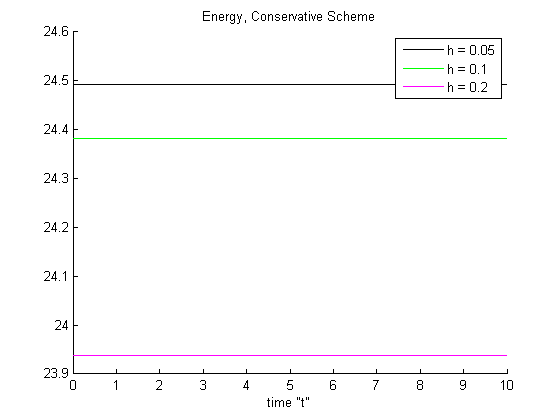
\includegraphics[width=\linewidth]{../amitans/figures/Energy_EnergySave_bt3_c045_x3O.png}	
	\end{minipage}
	\begin{minipage}[b]{0.48\linewidth}
		 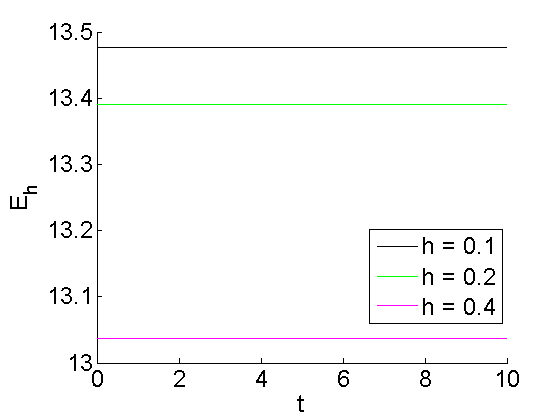
\includegraphics[width=\linewidth]{../amitans/figures/Energy_EnergySave_bt1_c090_x3O.png}
	\end{minipage}
\caption{Дискретната енергия на решението от Консервативната схема при Тест 1 (ляво) и Тест 2 (дясно) с апроксимационна грешка $O(|h|^2 + \tau^2)$ във времето $T_{\tau} = [0, 10]$.}
\label{EnOnly}
\end{figure}
Фигура \rf{EnOnly} показва развитиетно на дискретната Енергия за двата числени теста описани в Таблица \rf{tableP}. Вижда се, че независимо от големината на използваните стъпки по пространството $h = 0.05$, $h = 0.1$ и $h = 0.2$ при Тест 1 и $h = 0.1$, $h = 0.2$ и $h = 0.4$ при Тест 2, Енергията е константа величина за целия времеви период $T_{\tau} \in [0, 10]$. Стъпките по времето са описани в Таблица \rf{tableD}. Тези резултати в последствие ще се съпоставят с Енергията получена при метода на Тейлор. Пресметнат е и редът на сходимост за дискретната Енергия описан в Таблица \rf{tableD}, използвайки правилото на Рунге \rf{Runge}. Първата колона описва параметричната постановка съответно при Тест 1 и Тест 2. Втората колона е със стъпките по пространството и времето. Последните две колони дават информация за апроксимационните грешки и реда на сходимост получени съответно в $L_2$ и $L_\infty$ норми. Вижда се, че вторият ред на апроксимация отговаря на полученият втори ред на сходимост от таблицата при използваните норми.
%D
\begin{table}[ht]
\centering
\small
		\begin{tabular}{||c|l|ll|ll||}
			\hline
			\hline
      \multirow{2  }{*}{FDS}        & \multirow{2  }{*}{$h$, $\tau$}  &  	\multirow{2  }{*}{ $\Vert \bar{\bar{ E_i}} \Vert_{L_2}$ }	&Ред на	& \multirow{2  }{*}{ $\Vert \bar{\bar{ E_i}} \Vert_{L_\infty}$ } 		&Ред на   \\
	                                        &                                                & 							 					&  сход. 	& 								       					& сход. \\
   			\hline 
					\hline 
  $\beta=3$                &0.2, 0.005         &                    &                &                  &                   \\
   c=0.45                     &0.1, 0.0025         & 0.044442   &                & 0.444423  &                   \\
     $O(h^2 + \tau^ 2)$ &0.05, 0.00025  & 0.007831   & 2.50       & 0.110750  & 2.00   \\
	   \hline
			\hline 
       $\beta=1$           & 0.4, 0.002       &                   &           &                 &   \\
                  c=0.9       & 0.2, 0.001        & 0.051409   &          &0.363515  &   \\
  $O(h^2+ \tau^2)$  & 0.1, 0.0005       & 0.008939   & 2.52  &0.089393  & 2.02  \\
	   \hline
			\hline 
		\end{tabular}
		\caption{Скорост на сходимост на дискретната Енергия при Консервативната схема с нулево гранично условие и грешки от апроксимацията $O(h^{2} + \tau^2 )$. Грешките $\bar{\bar{ E_i}}$ са измерени в $L_2$ и $L_\infty$ норми.}
\label{tableD}
\end{table}

\section{ Метод на Тейлор }
Методът на Тейлор използва развитие в ред спрямо времевата променлива на търсената функция $u(x,y,t)$. Но за извеждането на крайните разлики за пресмятане на производните по пространството също се използва развитие в ред на Тейлор. Затова се предполага, че решението е $p+1$ кратна гладка функция спрямо всички аргументи $x$, $y$ и $t$, т.е. $u \in C^{p+1,p+1,p+1}(\Omega \times T)$ като при следващите изчисления описани по долу са използвани стойностите $p=2,4,6$. Непрекъснатият оператор на Лаплас в уравнение \rf{problemVC} се заменя с дискретния такъв, който е дефиниран в \rf{deltaHSingle}, което води до следната система от ОДУ:
\be \label{DiscreteEq}
\beta (I-\Delta_{h,p}) \frac{\partial^2 u}{\partial t^2}(x_i, y_j, t)=
 (I - \Delta_{h,p})\Delta_{h,p} u_{i, j}(t) + \Delta_{h,p} ( -\beta f( u_{i, j}(t) ) + (\beta-1) u_{i, j}(t) )
\ee
за всяка точка от мрежата $(x_i, y_j)$, където $i = 1..N_x-2$, $j=1..N_y-2$. За всяко едно ОДУ от системата се прави развитие в ред на Тейлор спрямо времевата променлива:
\begin{align} \label{TSe}
u(x_i, y_j, t+\tau) = u(x_i, y_j, t) + \tau \frac{ \partial u }{ \partial t }(x_i, y_j, t)  + ... 
\frac{ \tau^p }{ p! } \frac{ \partial^p u }{ \partial t^p }(x_i, y_j, t) + O(\tau^{p+1})
\end{align}
при $p \ge 2$. Всяка една от производните по времето в \rf{TSe} се изчислява посредством диференциране на \rf{DiscreteEq}
\begin{align}\label{discreteDer}
&\frac{\partial^s u}{\partial t^s}(x_i, y_j, t)= \frac{1}{\beta} \Delta_{h,p} \frac{\partial^{s-2} u}{\partial t^{s-2}} u_{i, j}(t) + \nonumber \\ 
&+\frac{1}{\beta} (I-\Delta_{h,p})^{-1} \Delta_{h,p} \frac{\partial^{s-2} u}{\partial t^{s-2}} ( -\beta f( u_{i, j}(t) ) + (\beta-1) u_{i, j}(t) ) 
\end{align}
при $s \ge 2$. За обръщането на оператора $(I-\Delta_{h,p})^{-1}$ се използват Fast Poisson Solvers. Редът на апроксимация по времето зависи от броя на членовете $p+1$, които участват в реда на Тейлор. По този начин реда на апроксимация по времето и пространството е еднакъв и зависи от избора на $p$, което по-късно спомага за тестването на сходимостта. Всяка точка от мрежата представлява начало на крива, чиято траектория се описва с развитието на Тейлор \rf{TSe}. Изчисляването на формула \rf{TSe} е рекурсивен процес като всеки член от сумата се пресмята отделно. Например, при $t=0$ първите два члена са известни от началното условие ($u_0$, $u_1$), а третият се получава чрез дискретното уравнение \rf{DiscreteEq}.  Следващият член в реда на Тейлор \rf{TSe} - третата производна по времето от \rf{discreteDer} и $s=3$ - изглежда по следния начин:
\begin{align} \label{der3}
 &\frac{\partial^3 u}{\partial t^3}(x_i, y_j, t) = \frac{1}{\beta}\Delta_{h,p} \frac{\partial}{\partial t}u_{i, j}(t) + \nonumber\\
&+ \frac{1}{\beta} (I-\Delta_{h,p})^{-1}\Delta_{h,p} \left( -2 \alpha \beta \: u_{i, j}(t) \frac{\partial}{\partial t}u_{i, j}(t) +  (\beta-1) \frac{\partial}{\partial t} u_{i, j}(t) \right).
\end{align}
За четвъртата производна по времето от \rf{discreteDer} при $s=4$ се получава:
\begin{align} \label{der4}
&\frac{\partial^4 u}{\partial t^4}(x_i, y_j, t) = \frac{1}{\beta}\Delta_{h,p} \frac{\partial^2}{\partial t^2}u_{i, j}(t) +   \nonumber\\
& \frac{1}{\beta}(I-\Delta_{h,p})^{-1}\Delta_{h,p} \left( -2 \alpha \beta \:  u_{i, j}(t)\frac{\partial^2}{\partial t^2}u_{i, j}(t) -2 \alpha \beta \: \left( \frac{\partial}{\partial t}u_{i, j}(t) \right)^2 + \right. \nonumber\\
&\quad \quad \quad \quad \quad \quad \quad \quad \quad \quad \quad \quad \quad \quad \quad \quad \quad \quad \quad \quad \left. +  (\beta-1) \frac{\partial^2}{\partial t^2} u_{i, j}(t) \right) .
\end{align}
В този случай дясната страна зависи от $u_{i, j}(t), \frac{\partial}{\partial t}u_{i, j}(t) и \frac{\partial^2}{\partial t^2}u_{i, j}(t)$ като последния член се получава от \rf{discreteDer} при $s=2$. Пресмятането на производните е итеративен процес, където например петата производна зависи от третата, втората, първата и нулевата, третата зависи от първата и нулевата. Тук е важно да се отбележи, че е необходимо да се пресметне и развитието в ред на Тейлор за първата производна по времето
\begin{align} \label{TSeDer}
\frac{ \partial}{ \partial t }u(x_i, y_j, t+\tau) = \frac{ \partial u }{ \partial t }(x_i, y_j, t) + \tau \frac{ \partial^2 u }{ \partial t^2 }(x_i, y_j, t)  + ... 
\nonumber\\
\frac{ \tau^p }{ p! } \frac{ \partial^{p+1} u }{ \partial t^{p+1} }(x_i, y_j, t) + O(\tau^{p+1})
\end{align}
което има същия ред на апроксимация спрямо \rf{TSe}. Това е необходимо, тъй като решението на по-следващия слой по времето $t+2\tau$ зависи от двойката ($u(t+\tau)$, $u_t(t+\tau)$), която служи като базис и всички по-високи производни могат да се изразят единствено чрез нея. След като всички необходими производни са пресметнати се заместват в уравнение \rf{TSe}, за да се получи решението на следващия слой по времето $t+\tau$, със следните локални апроксимации: за $p=2$ имаме $O(|h|^2 + \tau^3)$, за $p=4$ - $O(|h|^4 + \tau^5)$ и за $p=6$ - $O(|h|^6 + \tau^7)$. Понеже редът на Тейлор трябва да се пресметне на всеки слой по времето, локалната грешка акумулира с $N_t - 1 = T/\tau$, за да се получи $O(|h|^p + T \tau^p)$.

\subsection{Алгоритмични стъпки при метода на Тейлор}

Следващия запис дефинира стъпките при имплементацията на числения алгоритъм.
\\
1) Препроцесор
\par
1.1) зареждат се началните данни $V^{(0)}$ и $\frac{\partial}{\partial t} V^{(0)}$ (вече изчислени) като резултат от елиптичната задача,
\par
1.2) за конкретен избор на апроксимация $p$ се изчисляват:
\par
1.2.1) собствените стойности $D_x$, $D_y$ и вектори $S_x$, $S_y$ съответно на матриците $(\Delta_{h,p,x})^T$ и $(\Delta_{h,p,y})^T$, 
\par
1.2.2) обратните матрици $(S_x^T)^{-1}$, $S_y^{-1}$,
\\
2) Процесор $(k \rightarrow k+1)$. На всяка стъпка по времето $k\tau \in T_\tau$ се извършват следните операции:
\par
2.1) пресмятат производните по времето от втората до $p+1$-та ($s=2,..p+1$) използвайки \rf{discreteDer}:
\par
2.1.1) за целта първо се намират производните по времето само на нелинейната част на текущия ($k$-тия) слой по времето:
\begin{align*}
\bar f (V^{(k)}) = -f(V^{(k)}) + (\beta-1)V^{(k)} \\
B_{s} = \Delta_{h,p,y} * \frac{\partial^{s-2}}{\partial t^{s-2}} \bar f (V^{(k)}) + \frac{\partial^{s-2}}{\partial t^{s-2}}  \bar f (V^{(k)}) * (\Delta_{h,p,x})^T 
\end{align*}
\par
2.1.2) пресмятат се следните изрази:
\be\label{rightSide}
\Delta_{h,p}^{-1} B_{s}, \quad s=2,..p+1,
\ee
имайки предвид техниката за обръщане на двумерния дискретен оператор на Лаплас $\Delta_{h,p}$ (FPS). Това става посредством изчисленията на:
\par
2.1.2.1) субституцията \rf{subst} $X_h = S_x^T * V^{(k)} * S_y$,
\par
2.1.2.1) $X_h$ посредстовм формула \rf{fpp4Ext},
\par
2.1.2.3) обратната субституция \rf{substInv} $V^{(k)} = S_x^{-T} * X_h * S_y^{-1}$.
\par
2.1.3) изчисляват се и линейните части в \rf{discreteDer} и се сумират с нелинейните такива от \rf{rightSide}.
\par
2.2) резултатите от производните \rf{discreteDer} при $s=2,..p+1$ се заместват в редовете на Тейлор \rf{TSe} и \rf{TSeDer}, за да се получи неизвестната функция на горния слой по времето $u(t+\tau)$ заедно с $ \frac{\partial}{\partial t}u(t+\tau)$.
\par
2.3) дискретните стойности на масата $E_h(V^{(k)})$ и интеграла $D_h(V^{(k)})$ от решението.
\\
Сложността на алгоритъма 
$$ O(N_x N_y \bar \epsilon N_t ) $$
до голяма степен зависи от големината на областа, в която се разглежда числената задача, където $N_x N_y$ е броя на точките в $\Omega_h$, $\bar\epsilon \in (0, max(N_x,N_y) )$ и $N_t -1= T/\tau$. Повечето от изчислителното време се отделя за обръщане на оператора $I-\Delta_{h,p}$ в уравнение \rf{discreteDer}, което е необходимо за умноженията на матриците в стъпки 2.1.2.1) и 2.1.2.3). И в двата случая, присъстват умножения на матрици $N_y \times N_y$ с  $N_y \times N_x$ и $N_y \times N_x$ с  $N_x \times N_x$, при които сметки, изчислителната сложност се оценя на $ O( N_x N_y \bar\epsilon)$ (\cite{ref26}, \cite{ref27}). Избора на $p$, който е направен тук увеличава сложността с константа. Операциите в 2.1.2.1) и 2.1.2.3) се извършват на всяка стъпка по времето, т.е. изчислителната сложност зависи и от броя на слоевете по времето $N_t$.

\section{Числени резултати}
В тази част са представени резултати от имплементираните методи за хиперболичната задача.
Първоначално е представен редът на сходимост на дискретните решение и енергия получени от метода на Тейлор. Дискретните енергия и маса се пресмятат на всяка стъпка по времето и са вектори с дължина $N_t - 1$. Направени са допълнителни изчисления върху области с по-големи размери и по-голяма стъпка $h$, за да се обясни нарастването при масата. При Консервативната схема, енергията е получена чрез формула \rf{en_norm}, а при метода на Тейлор с правилата на трапците, Симпсън и Буул съответно с грешка от апроксимациите $O(h^{2} + \tau^2 )$, $O(h^{4} + \tau^4 )$ и $O(h^{6} + \tau^6 )$. Най-накрая са сравнени решенията между двата различни подхода. 

\subsection{Ред на сходимост при комбинацията от метода на Тейлор и метода на правите}
В таблица \ref{tableA} е представен редът на сходимост на численото решение. При метода на Тейлор са използвани апроксимации от втори, четвърти и шести ред, т.е. $p=2,4,6$ за Тест 1 и Тест 2 от първата колона в таблицата. Тук отново са направени изчисления върху три вложени мрежи с различни стъпки по времето и пространстово, които са показани във втората колона. В следващите две колони са представени апроксимационните грешки $\Vert \bar E_i \Vert_{L_2} $ и $\Vert \bar E_i \Vert_{L_\infty}$ заедно със съответните стойности за реда на сходимост като последните отговарят на приложения ред на апроксимация. Само при Тест 2, $O(h^6 + \tau^6)$ и $L_2$ норма, сходимостта $4.86$ е малко по-ниска от очакваното. Този резултат се отдава на нулевото гранично условие заедно с използвания седем точков шаблон по границата при апроксимация $O(h^6 + \tau^6)$.
%A
\begin{table}[ht]
\centering
\small
		\begin{tabular}{||c|l|ll|ll||}
			\hline
			\hline


      \multirow{2  }{*}{FDS}        & \multirow{2  }{*}{$h$, $\tau$}  &	\multirow{2  }{*}{  $\Vert \bar E_i \Vert_{L_2} $ } 	&Ред на & \multirow{2  }{*}{  $\Vert \bar E_i \Vert_{L_\infty}$ }	&Ред на   \\
	                                        &                                                &    										&  сход. & 										& сход. \\
   			\hline 
					\hline 
  $\beta=3$                &0.2, 0.001          &              &              &                     &      \\
   c=0.45                     &0.1, 0.0005          &0.989414 &            &1.043641    &       \\
     $O(h^2 + \tau^ 2)$ &0.05, 0.00025   & 0.344813 & 1.52    &0.355511    &  1.55      \\
			\hline 
  $\beta=3$               &0.2, 0.02       &              &            &                     &      \\
   c=0.45                    &0.1, 0.01      &0.191224 &            &0.193874    &       \\
     $O(h^4+ \tau^4)$ &0.05, 0.005&0.013029 & 3.87   &0.013656     &3.82       \\
			\hline 
  $\beta=3$               &0.2, 0.02       &                &            &                     &      \\
     c=0.45                 &0.1, 0.01        &0.032671 &            &  0.033626    &       \\
     $O(h^6+ \tau^6)$ &0.05, 0.005 &0.000598 &5.77     & 0.000635    & 5.72       \\
	   \hline
			\hline 
       $\beta=1$       &0.4, 0.002        &             &            &           &   \\
                  c=0.9    &0.2, 0.001       &  0.20366   &            &0.075854 &   \\
  $O(h^2+ \tau^2)$ &0.1, 0.0005   &0.048320   &2.07  &0.022307  & 1.77 \\
			\hline
      $\beta=1$               &0.4, 0.04    &            &               &             &    \\
       c=0.9                     &0.2, 0.02     & 0.028275   &        &  0.013518   &   \\
       $O(h^4+ \tau^4)$ &0.1, 0.01   &0.001812 & 3.96  & 0.000971  & 3.80  \\
    \hline
  $\beta=1$     &0.4, 0.04   &            &          &                  &      \\
      c=0.9                    &0.2, 0.02   &0.006734 &           & 0.003338      &       \\
     $O(h^6+ \tau^6)$ &0.1, 0.01 & 0.000232 &4.86 & 0.000069  & 5.60        \\
	   \hline
			\hline 
		\end{tabular}
		\caption{Скорост на сходимост на численото решение при метода на Тейлор с нулево гранично условие и грешки от апроксимацията $O(h^{2} + \tau^2 )$, $O(h^{4} + \tau^4 )$ и $O(h^{6} + \tau^6 )$. Грешките $\bar E_i$ са измерени в $L_2$ и $L_\infty$ норми.}
\label{tableA}
\end{table}
Таблица \ref{tableB} е аналогична с Таблица \ref{tableA}, но показва скоростта на сходимост на дискретната Енергия \rf{ex-en}. Резултатите от двете таблици са близки и съизмерими с използвания (втори, четвърти и шести) ред на апроксимация. Само при  Тест 2 и апроксимация $O(h^6 + \tau^6)$ стойностите за сходимостта $4.45$ и $4.68$ при $L_2$ и $L_{\infty}$ норми са по-малко от очакваното. Това поведение е аналогично с предишната Таблица \ref{tableA}, където само резулатът от $L_2$ нормата се отклонява и се отдава на нулевото гранично условие. Тъй като изчислението на Енергийния функционал \rf{ex-en} включва квадратурни формули, то неговото поведение изначало е сходно с това на $L_2$ нормата още преди да е приложена каквато и да е норма върху него. В случая на $O(h^2 + \tau^2)$  апроксимация и при двата теста е използвана по-малка стъпка $\tau = h/200$, което води до сходни по форма решения не само при трите вложени мрежи, но и при различните апроксимации. Ако се избере по-голяма стъпка (например $\tau = h/10$), разликите в решенията при $O(h^2 + \tau^2)$ и другите две апроксимации $O(h^4 + \tau^4)$ и $O(h^6 + \tau^6)$ са доста големи.

% When using zero boundary conditions all points on the finite difference stencil that are outside the numerical domain $\Omega_h$ are zeros. This creates a jagged solution surface on the boundary.

%B
\begin{table}[ht]
\centering
\small
		\begin{tabular}{||c|l|ll|ll||}
			\hline
			\hline
      \multirow{2  }{*}{FDS}        & \multirow{2  }{*}{$h$, $\tau$}  &  	\multirow{2  }{*}{ $\Vert \bar{\bar{ E_i}} \Vert_{L_2}$ }	&Ред на	& \multirow{2  }{*}{ $\Vert \bar{\bar{ E_i}} \Vert_{L_\infty}$ } 		&Ред на   \\
	                                        &                                                & 							 					&  сход. 	& 								       					& сход. \\
   			\hline 
					\hline 
  $\beta=3$                &0.2, 0.001         &              &            &                     &      \\
   c=0.45                     &0.1, 0.0005         &0.044442  &            &0.444425 &       \\
     $O(h^2 + \tau^ 2)$ &0.05, 0.00025  & 0.007831 & 2.50      & 0.110750     & 2.00      \\
			\hline 
  $\beta=3$               &0.2, 0.02       &                &            &                     &      \\
   c=0.45                    &0.1, 0.01      &0.018288 &            &0.072718   &       \\
     $O(h^4+ \tau^4)$ &0.05, 0.005  &0.000945 &4.27    &0.002997   &4.60      \\
			\hline 
  $\beta=3$               &0.2, 0.02       &                &            &                      &            \\
     c=0.45                 &0.1, 0.01        &0.027425 &            &  0.122934    &           \\
     $O(h^6+ \tau^6)$ &0.05, 0.005 &0.000318 & 6.42     & 0.001467     &6.38   \\
	   \hline
			\hline 
       $\beta=1$       &0.4, 0.002        &             &            &           &   \\
                  c=0.9    &0.2, 0.001       &  0.046343   &            &0.352955 &   \\
  $O(h^2+ \tau^2)$ &0.1, 0.0005   &0.007430   &2.64  &0.086470  & 2.02 \\
			\hline
      $\beta=1$               &0.4, 0.04    &            &               &             &    \\
       c=0.9                     &0.2, 0.02     & 0.023067   &        &  0.040550   &   \\
       $O(h^4+ \tau^4)$ &0.1, 0.01   &0.001411 & 4.03   & 0.003203  & 3.66  \\
    \hline
  $\beta=1$     &0.4, 0.04   &            &          &                  &      \\
      c=0.9                    &0.2, 0.02   &0.010898 &           & 0.032597      &       \\
     $O(h^6+ \tau^6)$ &0.1, 0.01 & 0.000496 &4.45 & 0.001266  & 4.68        \\
	   \hline
			\hline 
		\end{tabular}
		\caption{Скорост на сходимост на дискретната Енергия при метода на Тейлор с нулево гранично условие и грешки от апроксимацията $O(h^{2} + \tau^2 )$, $O(h^{4} + \tau^4 )$ и $O(h^{6} + \tau^6 )$. Грешките $\bar E_i$ са измерени в $L_2$ и $L_\infty$ норми.}
\label{tableB}
\end{table}
\FloatBarrier
\subsection{Числени резултати за Масата и Енергията}
Фигура \rf{Test1En} показва дискретните Маса и Енергия при Тест 1 изчислени посредством решенията от Консервативната схема и метода на Тейлор. 
Фигура \rf{Test2En} показва аналогични резултати, но при Тест 2. При метода на Тейлор, дискретната Маса и Енергия показани на Фигура \ref{Test1En} са пресметнати с три различни апроксимации - правило на трапците \rf{quadr2}, правило на Симпсън \rf{quadr4} и правило на Буул \rf{quadr6-2D}, съответно с грешка от апроксимацийте $O(h^2)$, $O(h^4)$ и $O(h^6)$. В случая на $O(|h|^2 +\tau^2)$ апроксимация, графиките на дискретните функции $E_h$ и $D_h$ получени от двата метода както при Тест 1 така и при Тест 2 се припокриват (черната линия и сините кръгчета). От тук може да се направят два важни извода. Първо, методът на Тейлор и Консервативната схема произвеждат качествено и количествено близки резултати за Масата и Енергията. Второ, енергията и при двата метода е константна величина спрямо времевата променлива. 
\begin{figure}[ht]\vspace{0.2cm}
	\begin{minipage}[b]{0.51\linewidth}
		 %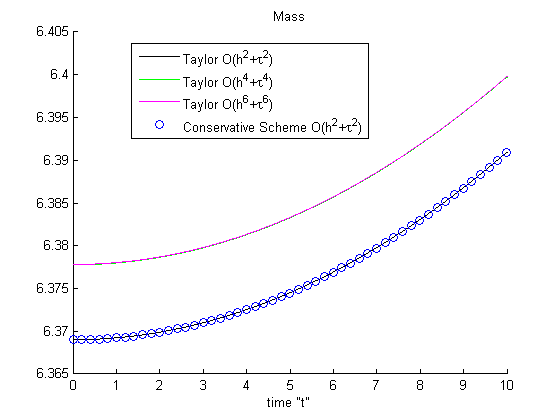
\includegraphics[width=\linewidth]{../amitans/figures/Mass_bt3_c045_h005_Taylor_Conservative.png}
		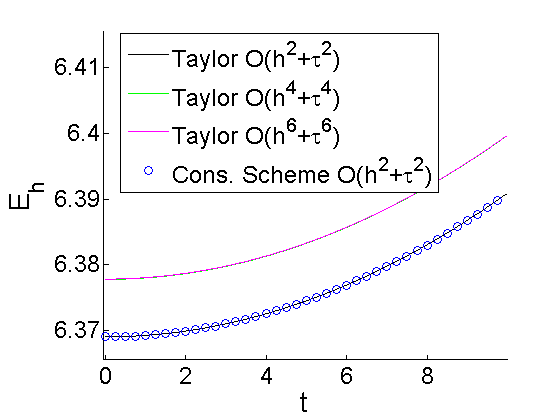
\includegraphics[width=\linewidth]{Mass/Mass_bt3_c045_h005_Taylor_Conservative.png}
	\end{minipage}	
	\begin{minipage}[b]{0.51\linewidth}
		%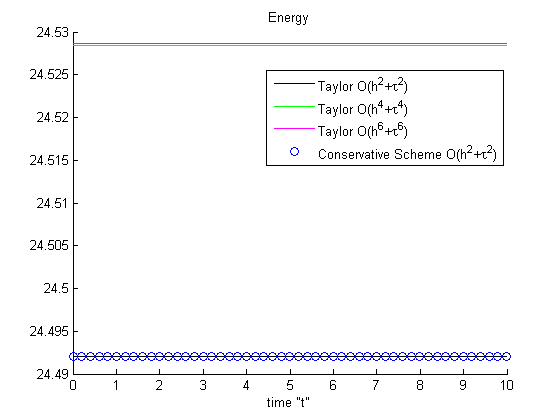
\includegraphics[width=\linewidth]{../amitans/figures/Energy_bt3_c045_h005_Taylor_Conservative.png}	
		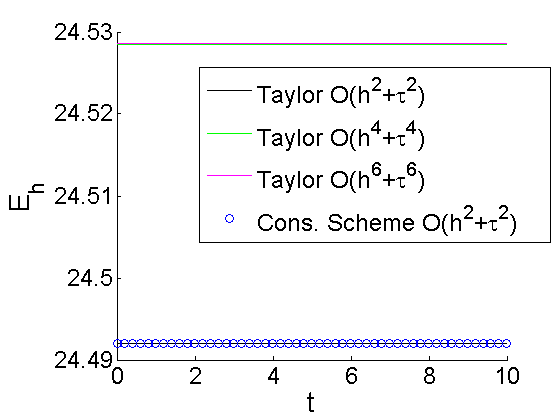
\includegraphics[width=\linewidth]{Energy/Energy_bt3_c045_h005_Taylor_Conservative.png}	
	\end{minipage}
\caption{Дискретните Маса (ляво) и Енергия (дясно) на решението като функция на времето до $T=10$ при Тест 1 и $O(|h|^2 + \tau^2)$.}
\label{Test1En}
\end{figure}
\FloatBarrier
При Масата се забелязва леко покачване за целия времеви интервал $[0, T]$, но то е пренебрежимо малко спрямо началната стойност. На този факт се обръща подробно внимание в следващата част.
\begin{figure}[ht]\vspace{0.2cm}
	\begin{minipage}[b]{0.51\linewidth}
		 %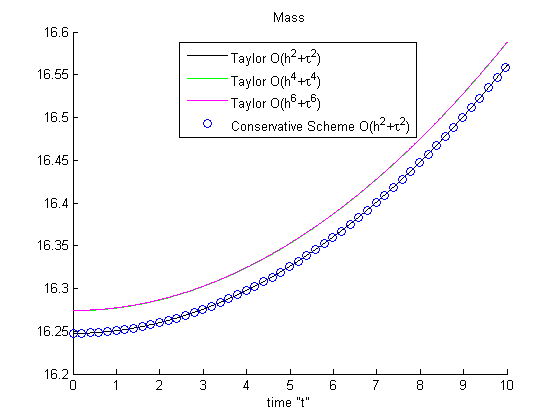
\includegraphics[width=\linewidth]{../amitans/figures/Mass_bt1_c090_h010_Taylor_Conservative.png}
		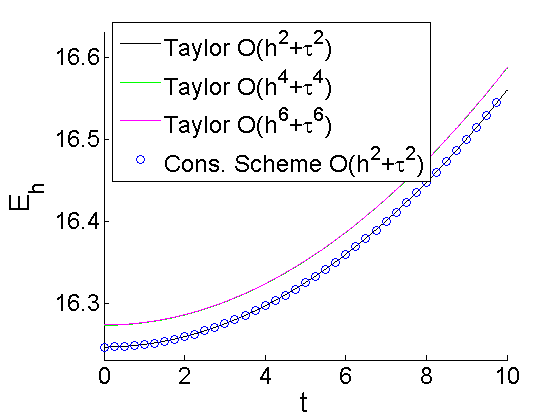
\includegraphics[width=\linewidth]{Mass/Mass_bt1_c090_h010_Taylor_Conservative.png}
	\end{minipage}	
	\begin{minipage}[b]{0.51\linewidth}
		%\includegraphics[width=\linewidth]{../amitans/figures/Energy_bt1_c090_h010_Taylor_Conservative.png}		
		\includegraphics[width=\linewidth]{Energy/Energy_bt1_c090_h010_Taylor_Conservative.png}				
	\end{minipage}
\caption{Масата (ляво) и Енергията (дясно) на решението като функция на времето до $T=10$ при Тест 2 и $O(|h|^2 + \tau^2)$.}
\label{Test2En}
\end{figure}
\FloatBarrier
 
\subsection{Числени резултати за Масата върху по-големи области $\Omega_h$}
Нека с $D_h^{**}$ означим процентното увеличение на Масата което се дефинира чрез
\be
D_h^{**} = 100 \times |D(t=0) - D(t=T)|/D(t=0).
\ee
При Тест 1 увеличението спрямо Масата в началния момент е $0.33\%$, а при Тест 2 е $1.8\%$ (Фигури \rf{Test1En}, \rf{Test2En}). Вижда се, че с подобряване степента на апроксимация, нарастването на масата остава непроменено. Промяна в големината на дискретните стъпки $h$ и $\tau=h/10, h/200$ (графиките са показани на Фигура \rf{Test2TEnMany}) също не води до съществена промяна във функцията на Масата спрямо показателя $D_h^{**}$. Затова в по-следващите изчисления, за да се обясни нейното поведението, се използва една и съща апроксимация - $O(h^6)$ с правилото на Буул - и фиксирана стъпки по пространството $h$ и времето $\tau$, а размерите на изчислителната област се увеличават.
%----------------------------------------------------------------------------------------------------------------------------------------------
%\iffalse
\begin{figure}[ht]\vspace{0.4cm}
	\begin{minipage}[b]{0.51\linewidth}
		 \includegraphics[width=\linewidth]{Mass/Mass_bt3_c045_h005_010_020_Taylor_Conservative.png}
	\end{minipage}	
	\begin{minipage}[b]{0.51\linewidth}
		\includegraphics[width=\linewidth]{Mass/Mass_bt1_c090_h010_020_040_Taylor_Conservative.png}
		
	\end{minipage}
\caption{Масата при Тест 1 (ляво) и Тест 2 (дясно) на решението като функция на времето до $T=10$, изчислена с различни стъпки при Консервативната схема с $O(|h|^2 + \tau^2)$ и метода на Тейлор с $O(|h|^6 + \tau^6)$.}
\label{Test2TEnMany}
\end{figure}
\FloatBarrier
%\fi
%----------------------------------------------------------------------------------------------------------------------------------------------
На Фигура \rf{Test1_2Mass} се вижда, че при увеличение на размерите на областта $\Omega_h$, увеличението на Масата намалява. При този числен експеримент, за генерирането на графиките, е използван метод на Тейлор с апроксимация от шести ред и най-големите стъпки по време и пространство ($h=0.2$ както при Тест 1 и $h=0.4$ както при Тест 2, а $\tau =  h/10$). На левия панел се вижда дискретната Маса изчислена върху три различни области съответно с големини 
\noindent 
\begin{equation*}
\begin{split}
& [-30, 30] \times [-27, 27], \nonumber\\
& [-60, 60] \times [-54, 54], \nonumber\\
& [-120, 120] \times [-108, 108] \nonumber\\
\end{split}
\end{equation*} 
\noindent 
при $\beta =  3$ и $c = 0.45$. Процентното увеличение на Масата спрямо увеличението на областта е измерено както следва $0.33\%$, $0.11\%$ и $0.06\%$. Аналогично, на десния панел, се вижда дискретната Маса изчислена върху три области с големини 
\noindent 
\begin{equation*}
\begin{split}
& [-128, 128] \times [-58, 58], \nonumber\\
& [-256, 256] \times [-116, 116], \nonumber\\
& [-512, 512] \times [-232, 232] \nonumber\\
\end{split}
\end{equation*} 
\noindent 
при $\beta =  1$ и $c = 0.9$. Тук процентното увеличение на Масата спрямо увеличението на областта е измерено както следва $1.80\%$, $0.70\%$ и $0.18\%$.
\begin{figure}[ht]\vspace{0.2cm}
	\begin{minipage}[b]{0.51\linewidth}
		\includegraphics[width=\linewidth]{Mass/MassTaylor_120_60_30_ZB1_bt3_c045_h020_O(h^6).png}
	\end{minipage}	
	\begin{minipage}[b]{0.51\linewidth}
		\includegraphics[width=\linewidth]{Mass/MassTaylor_512_256_128_ZB1_bt1_c090_h040_O(h^6).png}
		
	\end{minipage}
\caption{Масата от решението на Тейлор при $O(|h|^6 + \tau^6)$ апроксимация като функция на времето до $T=10$ върху три различни по големина области. Левия панел е при $\beta =  3$, $c = 0.45$, а десния панел е при $\beta =  1$, $c = 0.9$.}
\label{Test1_2Mass}
\end{figure}
\FloatBarrier
Тези резултати и разсъждения показват, че колкото е по-голяма областта $\Omega_h$, промяната в Масата отчетена чрез $D_h^{**}$, става все по-малка. Последното твърдение е в подкрепа на тезата, че $D_h$ е константна величина спрямо времевата променлива в непрекъсната област $\Omega$. 

\subsection{Числени резултати за формата на решението}
В тази част се разглежда формата на решението получена както с Консервативната схема, така и с метода на Тейлор. Стойностите на използваните параметри са описани в Таблица \ref{tableP}, когато $p=2$. Накратко, това са числени резултати от Тест 1 и Тест 2, при двата метода на решение, върху три вложени мрежи и с апроксимационни формули само от втори ред. Нека да означим с $uC$ и $uT$ двата класа от решения получени съответно с Консервативната схема \rf{consFDS} и метода на Тейлор \rf{TSe}. 
Фигури \ref{Test1_Diff} и \ref{Test2_Diff} илюстрират разликите между двата класа от решения получени съответно при Тест 1 и Тест 2. Графиките обхващат само централната (1/9) част от числената област $\Omega_h$, където отклоненията са по-големи. Ако разделим мислено $\Omega_h$ на по три равни по площ части, първо по дължина, а после и по ширина се получават девет еднакви правоъгълника като в картинките се разглежда средният.
\begin{figure}[ht]\vspace{0.2cm}
\centering
	\begin{minipage}[b]{0.32\linewidth}
		\includegraphics[width=\linewidth]{../amitans/figures/solution_30x45_bt3_c045_T0.png}
	\end{minipage}	
	\begin{minipage}[b]{0.32\linewidth}
		\includegraphics[width=\linewidth]{../amitans/figures/solution_30x45_bt3_c045_T6.png}
	\end{minipage}	
	\begin{minipage}[b]{0.32\linewidth}
		 \includegraphics[width=\linewidth]{../amitans/figures/solution_30x45_bt3_c045_T12.png}
	\end{minipage}
	\begin{minipage}[b]{0.32\linewidth}
		\includegraphics[width=\linewidth]{../amitans/figures/solution_30x45_bt3_c045_T18.png}
	\end{minipage}	
	\begin{minipage}[b]{0.32\linewidth}
		 \includegraphics[width=\linewidth]{../amitans/figures/solution_30x45_bt3_c045_T24.png}
	\end{minipage}
	\begin{minipage}[b]{0.32\linewidth}
		 \includegraphics[width=\linewidth]{../amitans/figures/solution_30x45_bt3_c045_T30.png}
	\end{minipage}
\caption{Числени резултати за една вълна при $\beta=3$ и $c = 0.45$ за времена $t=0,6,12,18,24,30$.}
\label{Wave1}
\end{figure}
\FloatBarrier
\begin{figure}[ht]\vspace{0.2cm}
\centering
	\begin{minipage}[b]{0.33\linewidth}
		\includegraphics[width=\linewidth]{../amitans/figures/solution_128x90_bt1_c090_T0.png}
	\end{minipage}	
	\begin{minipage}[b]{0.33\linewidth}
		\includegraphics[width=\linewidth]{../amitans/figures/solution_128x90_bt1_c090_T6.png}
	\end{minipage}	
	\begin{minipage}[b]{0.33\linewidth}
		 \includegraphics[width=\linewidth]{../amitans/figures/solution_128x90_bt1_c090_T12.png}
	\end{minipage}
	\begin{minipage}[b]{0.33\linewidth}
		\includegraphics[width=\linewidth]{../amitans/figures/solution_128x90_bt1_c090_T18.png}
	\end{minipage}	
	\begin{minipage}[b]{0.33\linewidth}
		 \includegraphics[width=\linewidth]{../amitans/figures/solution_128x90_bt1_c090_T24.png}
	\end{minipage}
	\begin{minipage}[b]{0.33\linewidth}
		 \includegraphics[width=\linewidth]{../amitans/figures/solution_128x90_bt1_c090_T30.png}
	\end{minipage}
\caption{Числени резултати за една вълна при $\beta=1$ и $c = 0.9$ за времена $t=0,6,12,18,24,30$.}
\label{Wave2}
\end{figure}
\FloatBarrier
\begin{figure}[ht]\vspace{0.4cm}
	\begin{minipage}[b]{0.32\linewidth}
		 \includegraphics[width=\linewidth]{../amitans/figures/compare_30_bt3_c045_h020.png}
	\end{minipage}	
	\begin{minipage}[b]{0.32\linewidth}
		\includegraphics[width=\linewidth]{../amitans/figures/compare_30_bt3_c045_h010.png}
	\end{minipage}	
	\begin{minipage}[b]{0.32\linewidth}		
		\includegraphics[width=\linewidth]{../amitans/figures/compare_30_bt3_c045_h005.png}
	\end{minipage}
\caption{Разликите $uC - uT$ между класовете от решения получени при Консервативната схема и метода на Тейлор при време $t=10$ и апроксимация $O(|h|^2 + \tau^2)$ при Тест 1. От ляво на дясно се променят стъпките както следва $h=0.2, 0.1, 0.05$.}
\label{Test1_Diff}
\end{figure}
\FloatBarrier
\begin{figure}[ht]\vspace{0.4cm}
	\begin{minipage}[b]{0.32\linewidth}
		\includegraphics[width=\linewidth]{../amitans/figures/compare_128_bt1_c09_h040.png}
	\end{minipage}	
	\begin{minipage}[b]{0.32\linewidth}
		\includegraphics[width=\linewidth]{../amitans/figures/compare_128_bt1_c09_h020.png}
	\end{minipage}	
	\begin{minipage}[b]{0.32\linewidth}
		\includegraphics[width=\linewidth]{../amitans/figures/compare_128_bt1_c09_h010.png}
	\end{minipage}
\caption{Разликите $uC - uT$  между класовете от решения получени при Консервативната схема и метода на Тейлор при време $t=10$ и апроксимация $O(|h|^2 + \tau^2)$ при Тест 2. От ляво на дясно се променят стъпките както следва $h=0.4, 0.2, 0.1$.}
\label{Test2_Diff}
\end{figure}
\FloatBarrier
Фигурите показват, че най-големите различия се проявяват около и в максимума на вълната. В допълнение към последните резултати е Таблица \ref{tableF}, която отново показва разликите $||uC - uT||_\kappa$ в  $L_2$ и ${L_\infty}$ норми. Първата колона от таблицата е за вида на числения тест, който е направен. Във втората колона са описани стъпките по пространството и времето. В третата и четвъртата са разликите от решенията между двата метода в $L_2$ и ${L_\infty}$ норми. Последната колона от таблицата е безкрайната норма на решението (което е максимума) при Консервативната схема. Наблюдава се, че при намаляване на дискретните стъпки $h$ и $\tau$ различията стават по-малки. Също така процентната разлика между двете решения дефинирана с безкайната норма
$$\frac{ ||uC - uT||_{L_\infty}} { ||uC||_{L_\infty} } \times 100$$
варира в интервала $[0.0001\%, 0.69\%]$ за всички случаи описани в таблицата. Аналогични резултати са получени и при процентната разлика дефинирана с $L_2$ нормата и затова те са пропуснати. Формите на решенията получени с Консервативната схема и метода на Тейлор са доста близки и от числените резултати се забелязва тенденцията, че разликата $||uC - uT||_\kappa$ клони към нула когато стъпките $h$ и $\tau$ са много малки.
%F
\begin{table}[ht]
\centering
\small
		\begin{tabular}{||c|l|l|l|l||}
			\hline
			\hline
      FDS        &$h$, $\tau$  &   $||uC - uT||$  in $L_2$     &  $||uC - uT||$ in $L_\infty$ & $||uC||$ in $L_\infty$ \\
   			\hline 
					\hline 
  $\beta=3$                   &0.2, 0.001         &  1.749e-05      &  1.965e-05  & 1.315448     \\
   c=0.45                        &0.1, 0.0005        &  8.109e-06       & 8.274e-06 &  1.862688     \\
     $O(h^2 + \tau^ 2)$ &0.05, 0.00025     & 2.460e-06         &2.502e-06  &   2.013184   \\
			\hline 
			\hline 
       $\beta=1$          &0.4, 0.002        & 0.009981     & 0.004560 & 0.656747   \\
                  c=0.9      &0.2, 0.001        & 0.005047      & 0.002373  & 0.673901   \\
  $O(h^2+ \tau^2)$ &0.1, 0.0005         & 0.002521      &0.001117 & 0.672231   \\
			\hline
	   \hline
			\hline 
		\end{tabular}
		\caption{Разлики $uC - uT$ между двата класа от решения получени от Консервативната схема и метода на Тейлор при време $t=10$ а апроксимация $O(|h|^2 + \tau^2)$. Разликите са измерени в $L_2$ и $L_\infty$ норми.}
\label{tableF}
\end{table}
\FloatBarrier
В този параграф се разглежда запазването на формата на решението във времевия интервал $[0, 10]$. Както и в по-горните случаи така и тук с помощта на параметричната Таблица \ref{tableP} се описват компютърните изчисления. Използван е метод на Тейлор с втори, четвърти и шести ред на апроксимация, а при всяка от апроксимациите са използвани три вложени мрежи. Резултатите са представени в Таблица \ref{tableG}. Първата колона описва вида на теста и апроксимацията. Втората колона представя стъпките по времето и пространството $h$ и $\tau$. В третата и четвъртата колони са показани разликите между решенията в началния $t=0$ и крайния  $t=10$ момент от време в  $L_2$ и $L_\infty$ норми. Вълната изминава разтояние равно на скоростта й умножена по крайното време $t=10$. В този случай максимума на решението се намира в $(0, 10 c) \in \Omega$, а в началния момент при $t=0$ максимума се намира в нулата $(0, 0) \in \Omega$. За съжаление при Тест 1, $h=0.2$ и Тест 2, $h=0.4$ максимума на решението при време $t=10$ не попада върху точка от мрежата. Затова са направени допълнителни итерации по времето с които да се отмести върха върху най-близката точка от мрежата $\Omega_h$. При Тест 1 ($c=0.45$) вълната изминава допълнително разтояние от 0.1 за време 2/9, което измества максимума в позиция $(0, 4.6) \in \Omega_h$. При Тест 2 ($c=0.9$) вълната изминава допълнително разтояние от 0.2 за време 2/9, което измества максимума в позиция $(0, 9.2) \in \Omega_h$. Разликата между двете решения $u^{(0)} - u^{(N_t)}$ може да се опише чрез матрица със следните коефициенти:
$$ \delta_{i,j} = u_{i,j}^{(0)} - u_{i,j+cT/h}^{(N_t)},$$
където $0 < i < N_x$ и $0 < j < N_y - cT/h$. 
%G
\begin{table}[ht]
\centering
\small
		\begin{tabular}{||c|l|l|l||}
			\hline
			\hline
      FDS        & $h$, $\tau$  & $||u^{(0)} - u^{(N_t)}||$ in $L_2$  & $||u^{(0)} - u^{(N_t)}||$ in $L_\infty$   \\
   		\hline 
			\hline
  $\beta=3$                &0.2, 0.001\footnote{Position of maximum is further adjusted to fit inside $\Omega_h$.}            & 1.494351 & 1.533173    \\
   c=0.45                     &0.1, 0.0005          & 0.466991 & 0.484011       \\
     $O(h^2 + \tau^ 2)$ &0.05, 0.00025   & 0.127641 & 0.132504      \\
			\hline 
  $\beta=3$               &0.2, 0.02 $^{\text{a}}$      &0.220560 & 0.230486       \\
   c=0.45                    &0.1, 0.01      &0.013762 & 0.014391        \\
     $O(h^4+ \tau^4)$ &0.05, 0.005&0.000877 & 0.000917         \\
			\hline 
  $\beta=3$               &0.2, 0.02 $^{\text{a}}$       &  0.035965 & 0.038039        \\
     c=0.45                 &0.1, 0.01        &0.000600 & 0.000633       \\
     $O(h^6+ \tau^6)$ &0.05, 0.005 &0.000010 & 0.000010          \\
	   \hline
			\hline 
       $\beta=1$       &0.4, 0.002 $^{\text{a}}$       & 0.244208 & 0.103833 \\
                  c=0.9    &0.2, 0.001       &  0.057175 & 0.026919  \\
  $O(h^2+ \tau^2)$ &0.1, 0.0005   & 0.013938 & 0.006622  \\
			\hline
      $\beta=1$               &0.4, 0.04 $^{\text{a}}$    &0.028546 & 0.012203 \\
       c=0.9                     &0.2, 0.02     & 0.001757 & 0.000958     \\
       $O(h^4+ \tau^4)$ &0.1, 0.01   & 0.000112 & 0.000061   \\
    \hline
  $\beta=1$                  &0.4, 0.04 $^{\text{a}}$   &0.006415 & 0.002792  \\
      c=0.9                    &0.2, 0.02   &0.000112 & 0.000065     \\
     $O(h^6+ \tau^6)$ &0.1, 0.01 & 0.000002 & 0.000001         \\
	   \hline
			\hline 
		\end{tabular}
		\caption{Разликата $||u^{(0)} - u^{(N_t)}||_\kappa$ в $L_2$ и $L_\infty$ норми между решенията в началния $t=0$ и крайния $t=10$ моменти от време. За резултатите от таблицата е използван единствено метода на Тейлор.}
\label{tableG}
\end{table}
\FloatBarrier
Таблица \ref{tableG} показва, че с намаляване на стъпките по пространството $h$ и времето $\tau$, разликата между разгледаните решения също намалява. В допълнение се вижда, че формата на вълната се запазва по-добре, когато степента на апроксимация $p$ на диференциалните оператори е по-висока. Последните разсъждения затвърждават очакването, че разликата във формата на решението $||u^{(0)} - u^{(N_t)}||_\kappa$ при различни времена клони към нула когато $h$ и $\tau$ са много малки.

\subsection{Числени резултати за максимума на решението}
В следния параграф се обръща внимание на максимума на решението, но при по-голям времеви интервал $[0, 30]$. Постановката за този числен експеримент е описана с помощта на Таблица \ref{tableP}, т.е. използван е метод на Тейлор с шести ред на апроксимация $p=6$, със стъпки $h=0.05$, $\tau = 0.001$ при Тест 1 и $h=0.2$,  $\tau=0.02$ при Тест 2. Крайното време е $T=30$, а големината на областта $\Omega_h$ е увеличена по $y$ оста за да обхване преместването на вълната изцяло, т.е. $L_y = 45$ при Тест 1 и $L_y = 90$ при Тест 2. Както вече е описано по-горе, точната позиция на максимума не винаги лежи върху точка от мрежата $\Omega_h$. Това води до назъбване на графиките, което се забелязва по-отчетливо на десния панел при Тест 2 на Фигура \ref{Maximum}. 
\begin{figure}\vspace{0.2cm}
	\centering
	\begin{minipage}[b]{0.40\linewidth}
		\includegraphics[width=\linewidth]{../amitans/figures/maximum_30_T30_bt3_c045_h005.png}
	\end{minipage}	
	\begin{minipage}[b]{0.40\linewidth}
		 \includegraphics[width=\linewidth]{../amitans/figures/maximum_30_T30_bt1_c090_h020.png}
	\end{minipage}
\caption{Развитие на максимума на решението върху по-голям интервал от време $[0, 30]$ при Тест 1 (ляв панел) и Тест 2 (десен панел).}
\label{Maximum}
\end{figure}
\FloatBarrier
За всеки от разработените методи са изчислени масата и енергията върху полученото решение. То, заедно с неговите свойства като маса, енергия и форма са сравнени. Изчисленията са направени върху три вложени мрежи, за да се изследва сходимостта на методите. Показано е, че решенията получени с метода на Тейлор и Консервативната схема са доста близки. Една от целите на статията е да покаже, че метода на Тейлор приложен към уравнението \rf{problemVC} също води до достатъчно добри резултати, а също така може да се приложи с по-висок ред на апроксимация, което води и до по-фино решение.

\begin{thebibliography}{99}

\bibitem{ref16} Angelow, K., Kolkovksa, N., Numercal Study of Traveling Wave Solutions to 2D Boussinesq Equation, {\it Serdica J. Computing}, \textbf{13} (2019), 1-16.

\bibitem{ref0} Boussinesq, J.V., Theorie des ondes et des remous qui se propagent le long d'un canal rectangulaire horizontal, en communiquant au liquide contenu dans ce canal des vitesses sensiblement pareilles de la surface au fond.  {\it Journal de Mathematiques Pures et Appliquees}, \textbf{17} (1872), 55-108.

\bibitem{ref21} Chertok, A., Christov, C.I., Kurganov, A., Central-Upwind Schemes for the Boussinesq Paradigm Equations,
{\it Computational Science and High Performance Computing IV, Notes Numer. Fluid Mech.}, \textbf{113} (2011), 267-281.

\bibitem{ref13}  Christou M. , Christov C.I.,
Galerkin spectral method for the 2D solitary waves of Boussinesq paradigm equation,
In: {\it Applications of Mathematics in Technical and Natural Sciences, Sozopol (Bulgaria)},
\emph{AIP Conference Proceedings}, \textbf{1186}, Issue 1 (2009), 217-225.

\bibitem{ref14}  Christou M. , Christov C.I.,
Fourier Galerkin method for 2D solitons of Boussinesq equation,
{\it Mathematics and Computers in Simulation} \textbf{74} (2007), 82-92.

\bibitem{ref1} Christov, C.I., An energy-consistent dispersive shallow-water model,  {\it Wave Motion}, \textbf{34} (2001), 161-174.

\bibitem{ref15} Christov, C.I., Choudhury, J., Perturbation solution for the 2D Boussinesq equation, {\it Mech. Res. Commun.}, \textbf{38} (2011), 274-281.

\bibitem{ref116}  C.I. Christov,
Numerical implementation of the asymptotic boundary conditions for steadily propagating 2D solitons of Boussinesq type equations,
{\it Mathematics and Computers in Simulation}, \textbf{82} (2012), 1079-1092.

\bibitem{ref117}  J. Choudhury, C.I. Christov,
2D solitary waves of Boussinesq equation, in ISIS International Symposium on Interdisciplinary Science, Natchitoches, October 6-8, 2004, {\it APS Conference Proceedings 755}, Washington, DC, 2005, pp 85-90.

\bibitem{ref4} Christov, I., Christov, C.I., Physical dynamics of quasi-particles in nonlinear wave equations,
{\it Physics Letters A}, \textbf{372}, Issue 4 (2008),  841-848.

\bibitem{ref20} Christov, C.I., Kolkovska, N., Vasileva, D., On the Numerical Simulation of Un-
steady Solutions for the 2D Boussinesq Paragigm Equation,
{\it In: I. Dimov, S. Dimova, N. Kolkovska (Eds.), Numerical Methods and Applications 2010},
\emph{Conference Proceedings}, \textbf{6046} (2010), 386–394.

\bibitem{ref23} Dimova M., Vasileva D., Comparison of Two Numerical Approaches to Boussinesq Paradigm Equation, 
{\it Lect. Notes Comput. Sci.}, \textbf{8236} (2013), 255-262.

\bibitem{Ch2011}
C.I.Christov, J. Choudhury, Perturbation solution  for the 2D Boussinesq equation,       
{\it Mech. Res. Commun.}, 38 (2011),  274 -- 281.

\bibitem{forn}
Fornberg, B., Generation of Finite Difference Formulas on Arbitrarily Spaced Grids, 
Math. Comput., 51(1988),  699 -- 706.

\bibitem{samarski} Samarskii, A., The Theory of Difference Schemes, Marcel Dekker Inc., New York, 2001.

\bibitem{ref22} Kolkovska, N., Angelow K., A Multicomponent Alternating Direction Method for Numerical Solving of Boussinesq Paradigm Equation,
In: {\it  I. Dimov, I., Farago, I., Vulkov, L. (eds.) NAA 2012},
\emph{Conference Proceedings}, \textbf{8236} (2013), 371–378.

\bibitem{ref25} Kolkovska N.,Two families of finite difference schemes for multidimensional Boussinesq paradigm equation, In:
{\it Applications of Mathematics in Technical and Natural Sciences,  Sozopol (Bulgaria)},
\emph{AIP Conference Proceedings}, \textbf{1301} (2010), 395.

\bibitem{ref260} G. H. Golub and C. F. Van Loan, Matrix Computations, 3/e, Johns Hopkins University, Press, Baltimore, 1996.

\bibitem{ref26} 
Strassen, Volker, Gaussian Elimination is not Optimal,
{\it Numer. Math.}, \textbf{13 (4)} (1969), 354–356, doi:10.1007/BF02165411. S2CID 121656251

\bibitem{ref27} Coppersmith, Don; Winograd, Shmuel., Matrix multiplication via arithmetic progressions,
{\it  Journal of Symbolic Computation}, \textbf{9 (3)} (1990), 251, doi:10.1016/S0747-7171(08)80013-2.

\bibitem{boole}
Zucker, Ruth, "Chapter 25.4.14: Numerical Interpolation, Differentiation, and Integration - Integration - Numerical Analysis". In Abramowitz, Milton; Stegun, Irene Ann (eds.). Handbook of Mathematical Functions with Formulas, Graphs, and Mathematical Tables. 
\it{Applied Mathematics Series} \textbf{55}  (1983), ISBN 978-0-486-61272-0.

\bibitem{ref25} Kolkovska N.,Two families of finite difference schemes for multidimensional Boussinesq paradigm equation, In:
{\it Applications of Mathematics in Technical and Natural Sciences,  Sozopol (Bulgaria)},
\emph{AIP Conference Proceedings}, \textbf{1301} (2010), 395.

\bibitem{ref1c0} Kolkovska N. Angelow K., Numerical computation of the critical energy constant for two-dimensional Boussinesq equations,
{\it Application of Mathematics in Technical and Natural Sciences, Albena (Bulgaria)},
\emph{AIP Conference Proceedings}  \textbf{1684} (2015), 080007.

\bibitem{ref2c0} Kolkovska N., Numerical Evaluation of 2D Ground States,
\emph{ EPJ Web of Conferences}, \textbf{108} (2016), 02032.

\bibitem{dani}
C. Christov, N. Kolkovska, D. Vasileva, On the numerical simulation of unsteady solutions for the 2D Boussinesq paradigm equation, LNCS, \textbf{8236}  (2011), 386.

\bibitem{milenaDani}
M.Dimova, D. Vasileva, Comparison of Two Numerical Approaches to Boussinesq Paradigm Equation, 
{\it Numerical Analysis and Its Applications. NAA 2012. Lecture Notes in Computer Science}, \textbf{8236}, (2013), 255.

\bibitem{ref31} B. Engquist and A. Majda, Absorbing boundary conditions for the numerical simulation of waves, {\it Math. Comp.}, \textbf{31} (1977), 629–651.

\bibitem{ref32}  C.I. Goldstein, A finite element method for solving Helmholtz type equations in waveguides and other unbounded domains,
{\it Math. Comp.}, \textbf{39} (1982), 309–324.

\bibitem{ref33}  H. Han, W. Bao, Error estimates for the finite element approximation of problems in unbounded domains,
{\it SIAM J. Numer. Anal.} \textbf{37}, \textbf{4} (2000), 1101–1119

\bibitem{ref34} T. Lyche, Fast Direct Solution of a Large Linear System,
\it{Numerical Linear Algebra and Matrix Factorizations, Texts in Computational Science and Engineering}, \textbf{22}, (2020), p 237-250 

\end{thebibliography}
\end{document}